\section{Anhang}

\subsection{Einleitung}
\subsubsection{Blockdiagramm}
\begin{figure}[htbp]
	\centering
	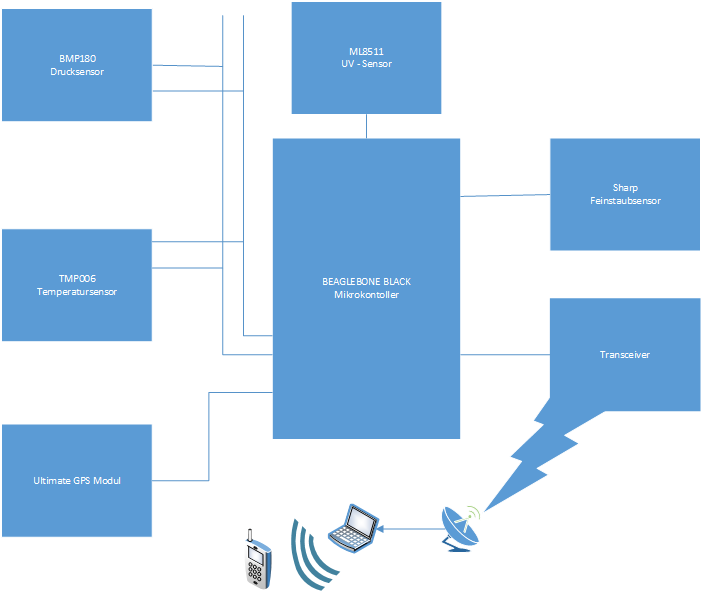
\includegraphics[width=0.8\textwidth]{8_Anhang/Blockdiagramm.png}
	\caption{Blockdiagramm vom CANSAT}
	\label{blockdiagramm}
\end{figure}

\newpage

\subsection{GANTT-Diagramme}
\subsubsection {Hardware-GANTT}
\begin{figure}[htbp]
	\centering
	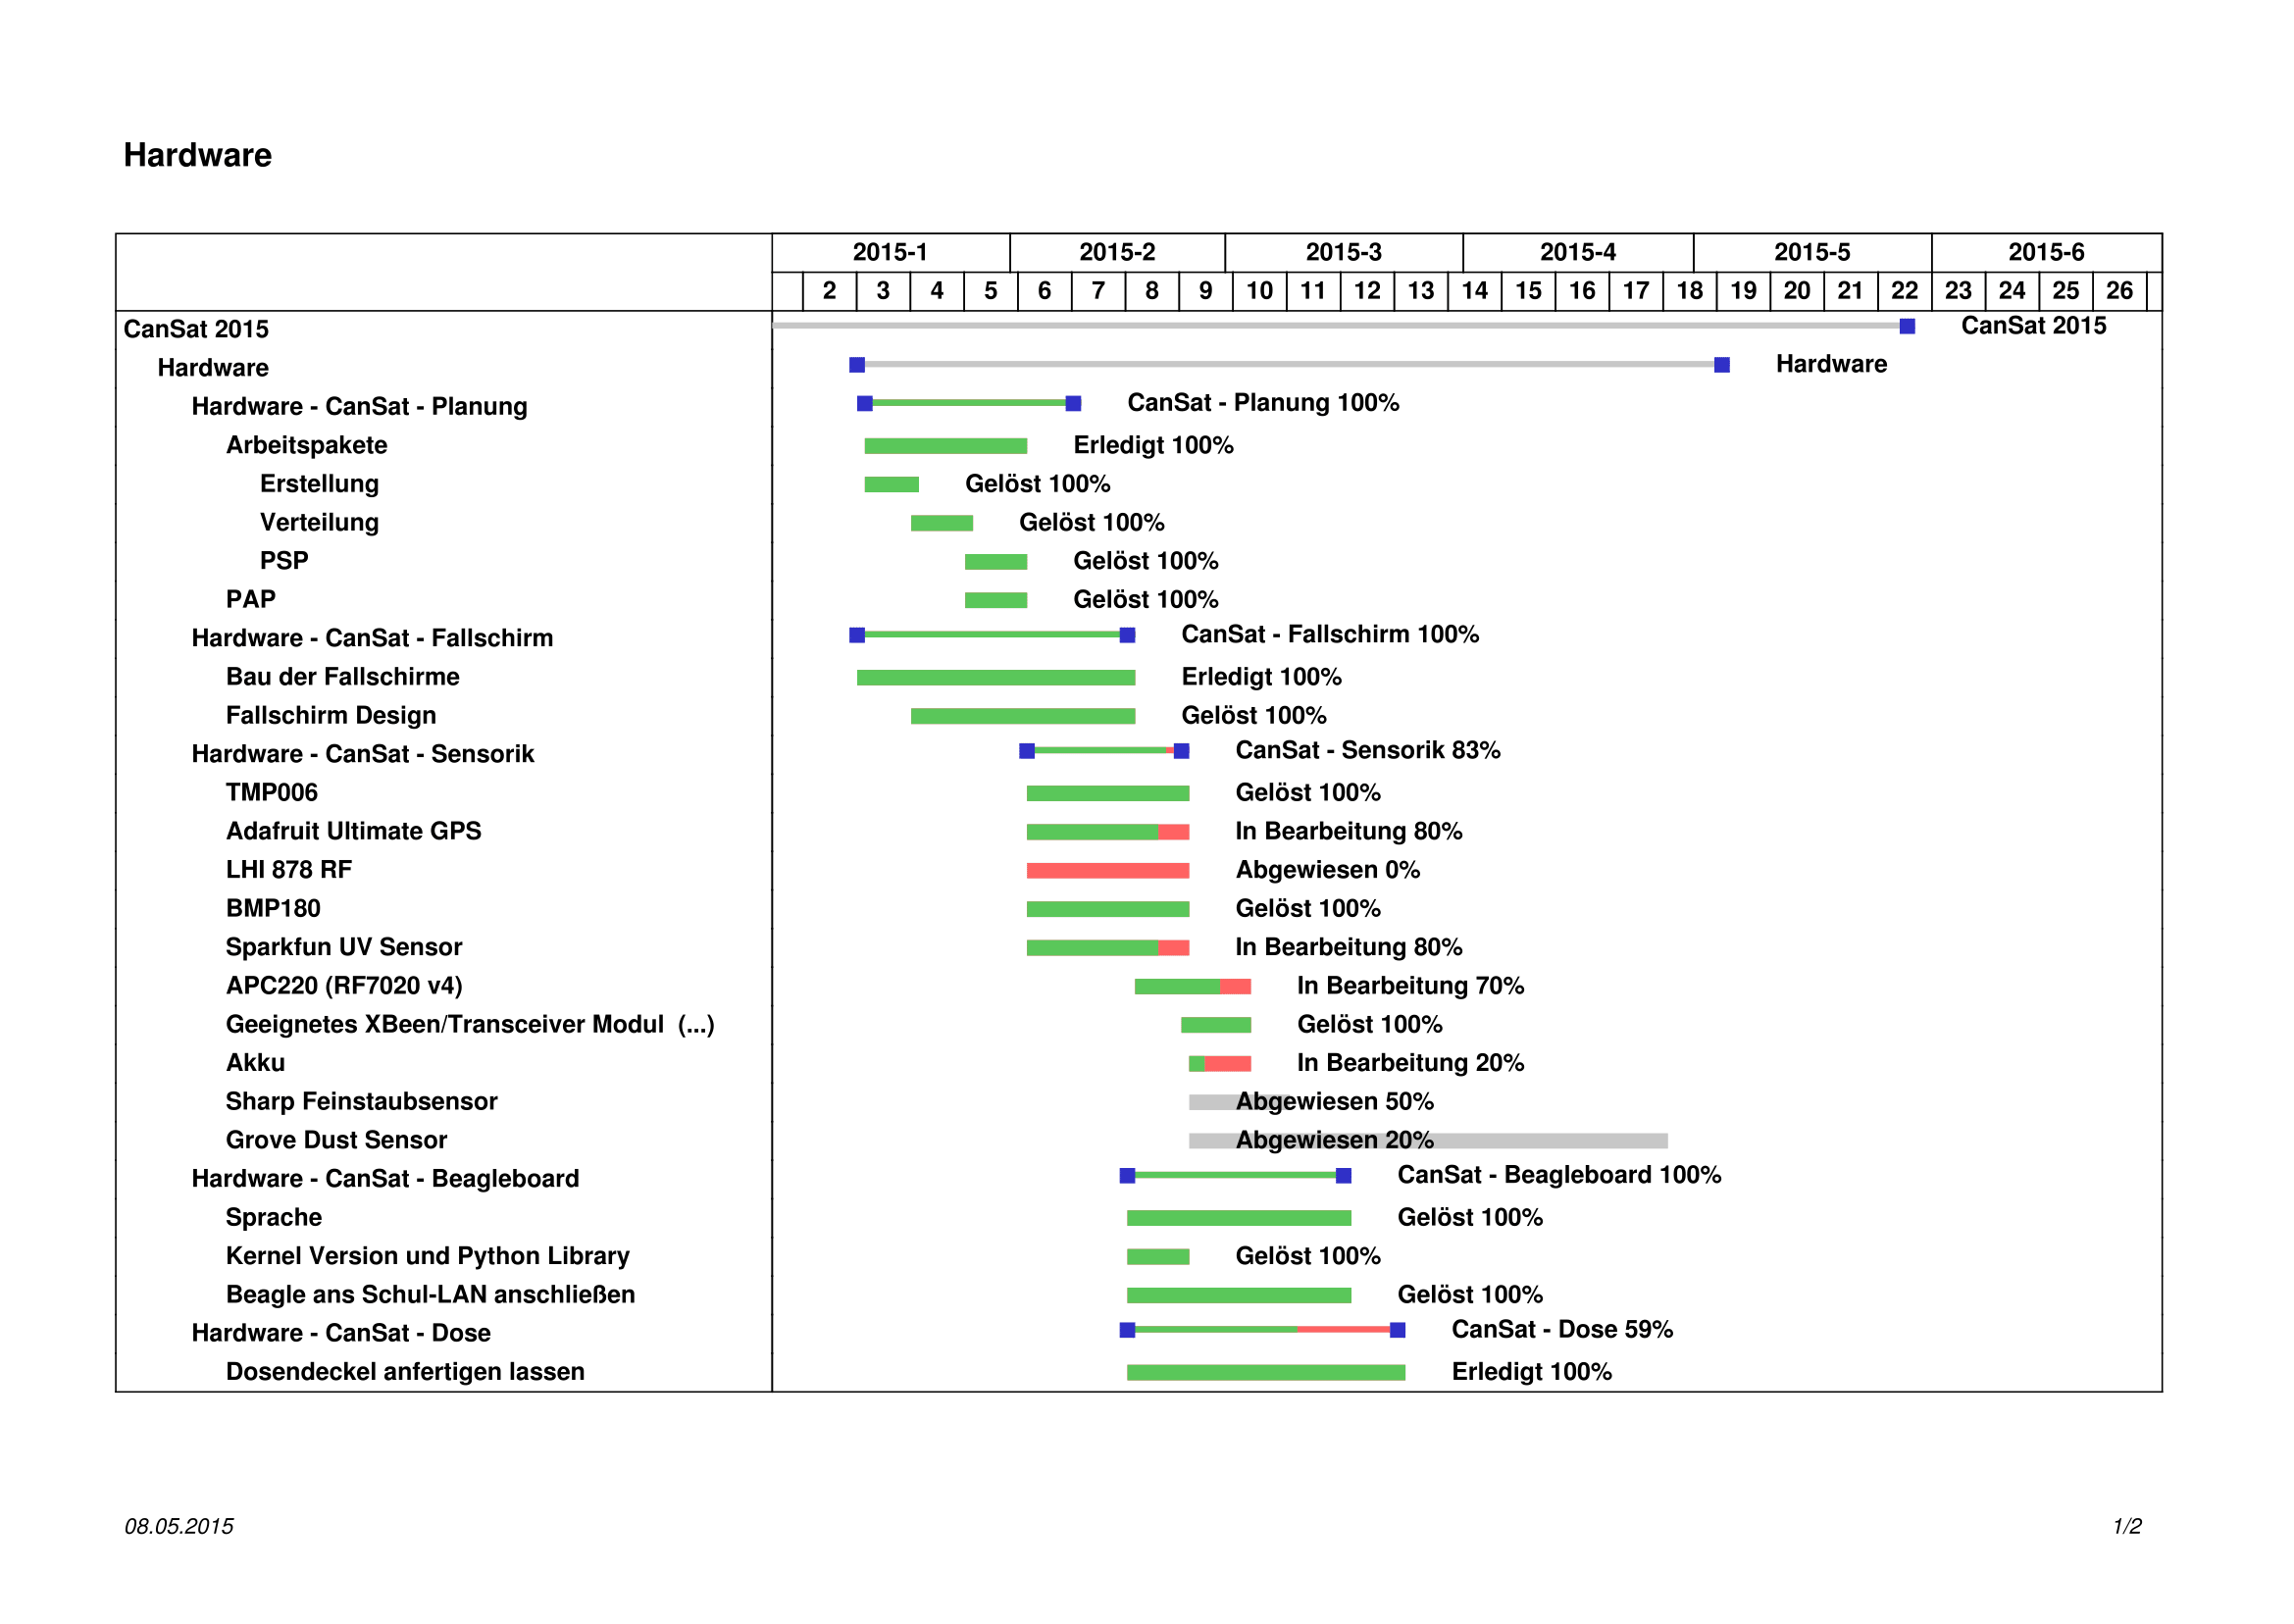
\includegraphics[trim = 10mm 50mm 20mm 65mm, clip,width=0.8\textwidth]{8_Anhang/hardware-gantt-1.png}
	\label{gantt_hardware_1}
\end{figure}
\vspace{-2cm}
\begin{figure}[htbp]
	\centering
	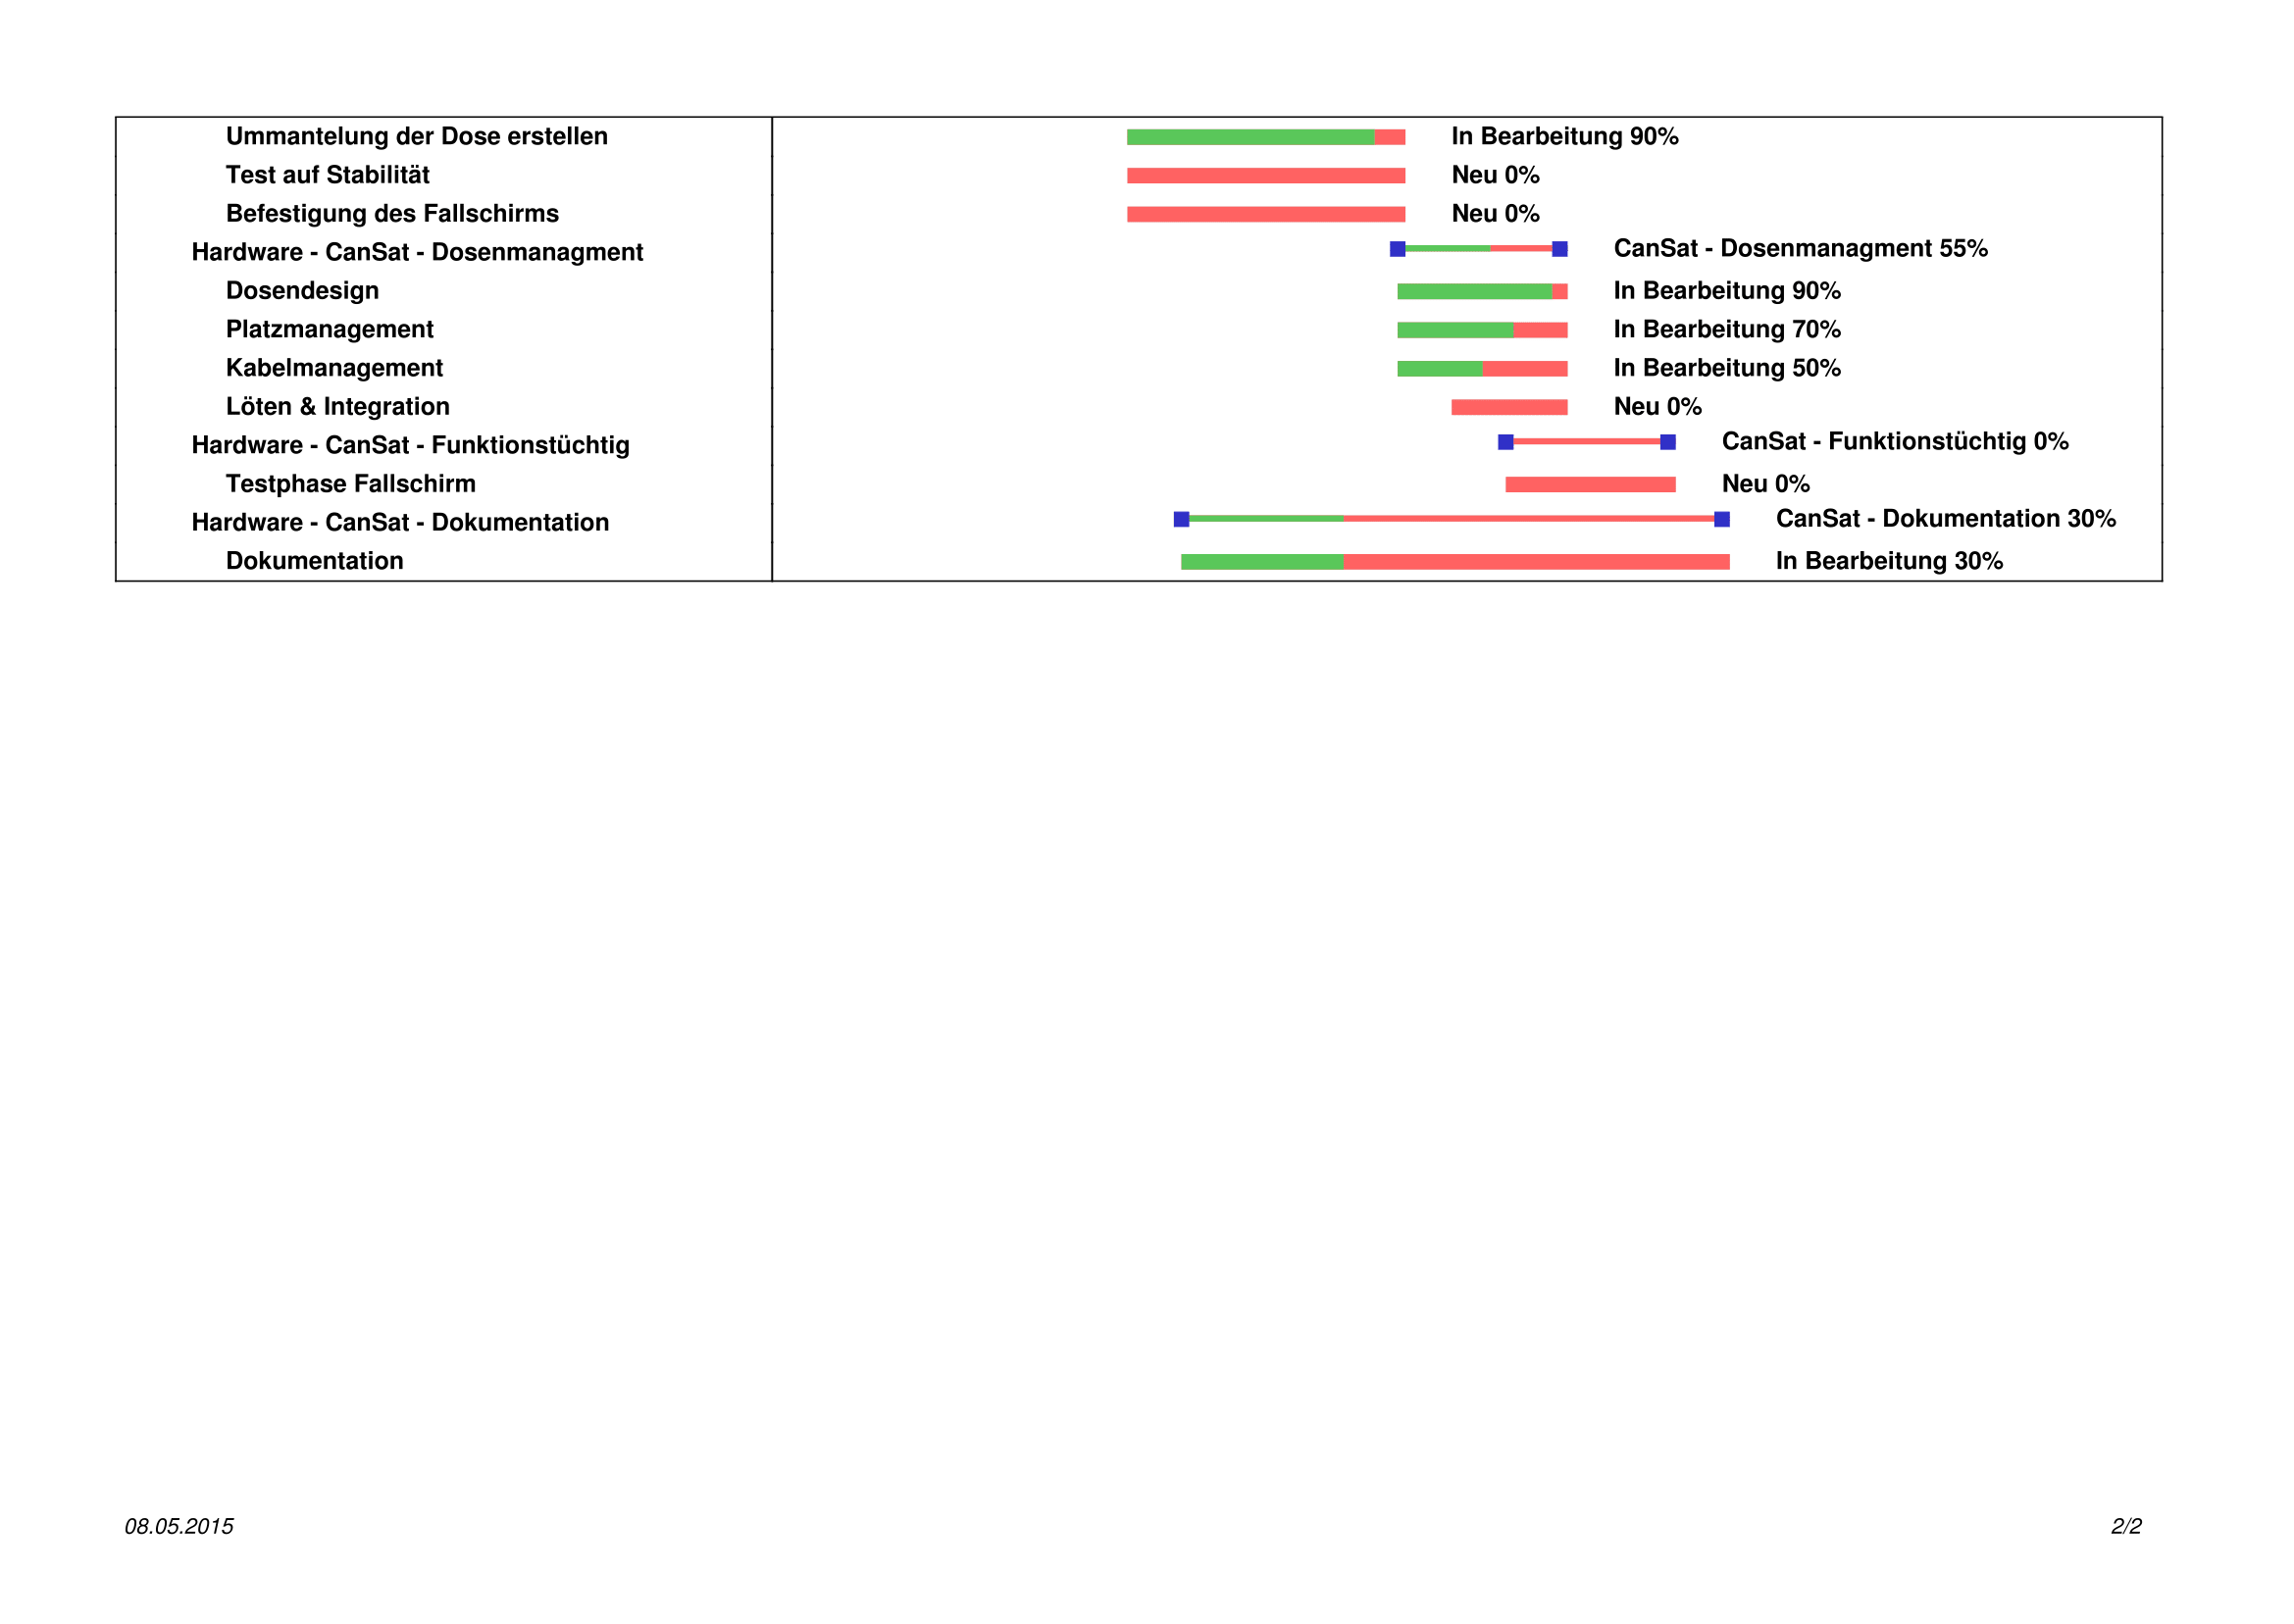
\includegraphics[trim = 11mm 350mm 20mm 40mm, clip,width=0.8\textwidth]{8_Anhang/hardware-gantt-2.png}
	\caption{Das GANTT-Diagramm der Hardware Gruppe}
	\label{gantt_hardware_2}
\end{figure}

\newpage
\subsubsection {Bodenstation-GANTT}
\begin{figure}[H]
	\centering
	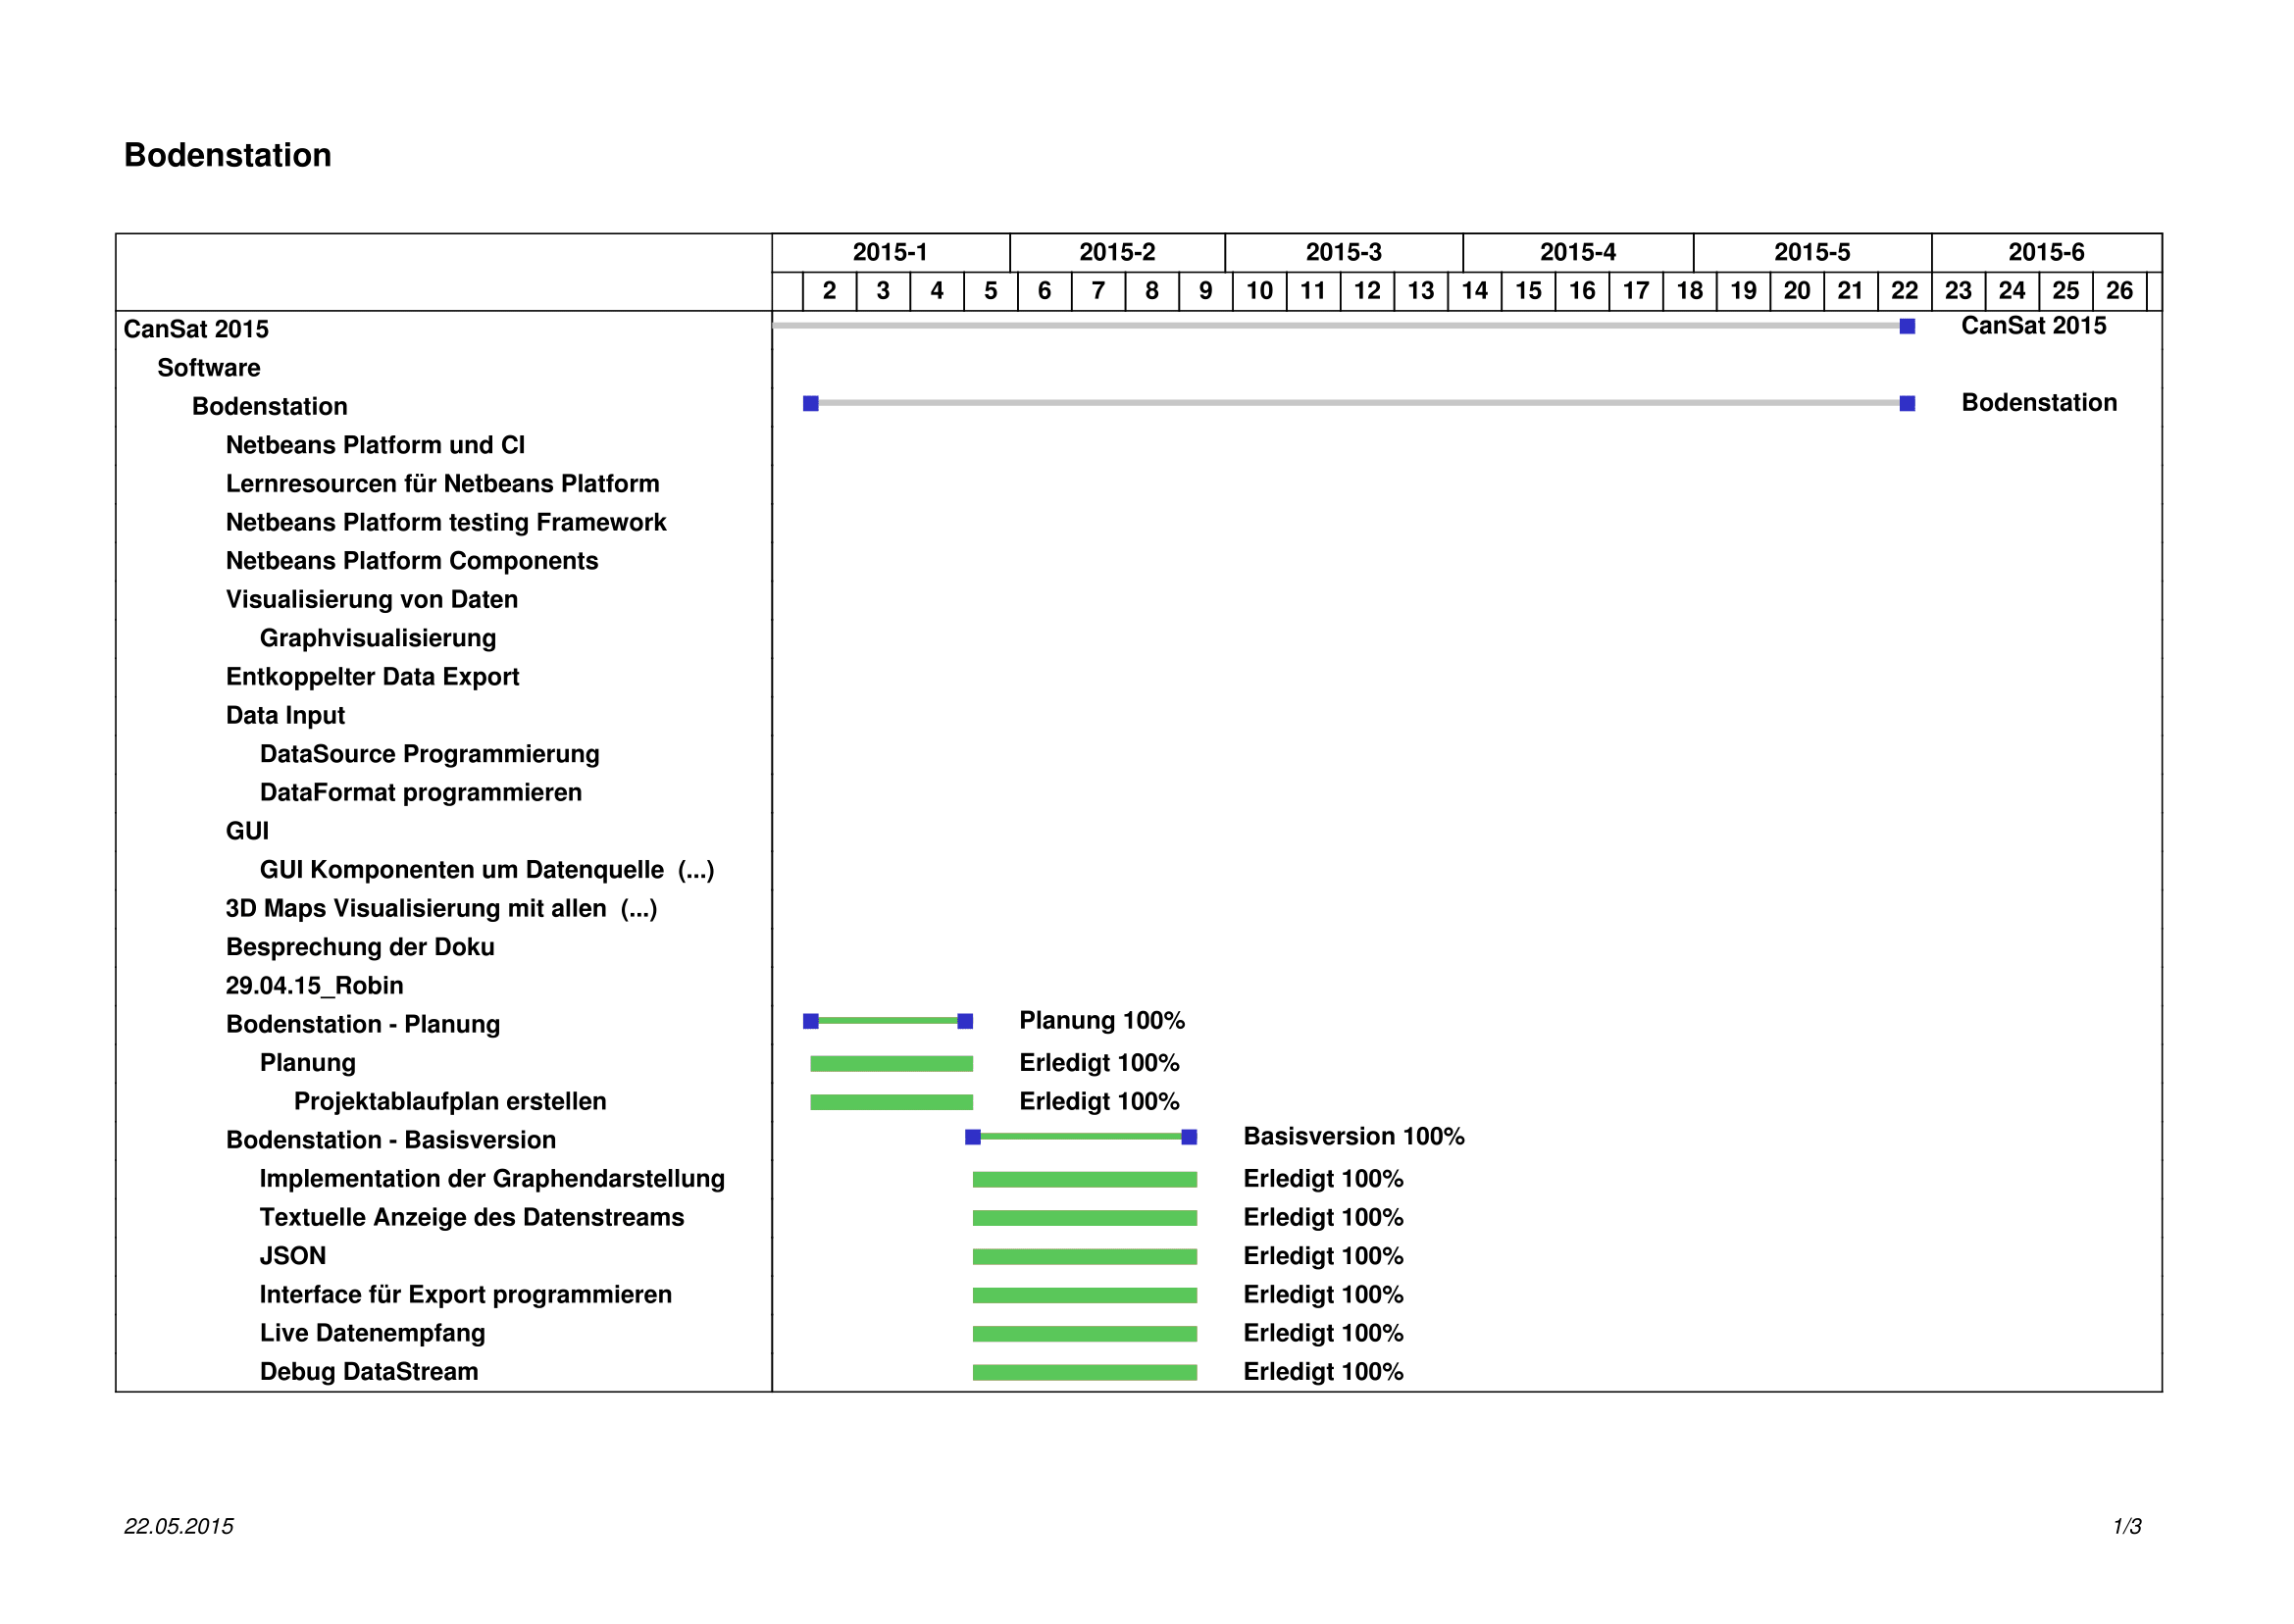
\includegraphics[trim = 25mm 50mm 46mm 65mm, clip,width=0.8\textwidth]{8_Anhang/bodenstation-gantt-1.png}
	\label{gantt_hardware_1}
\end{figure}
\vspace{-1,3cm}
\begin{figure}[H]
	\centering
	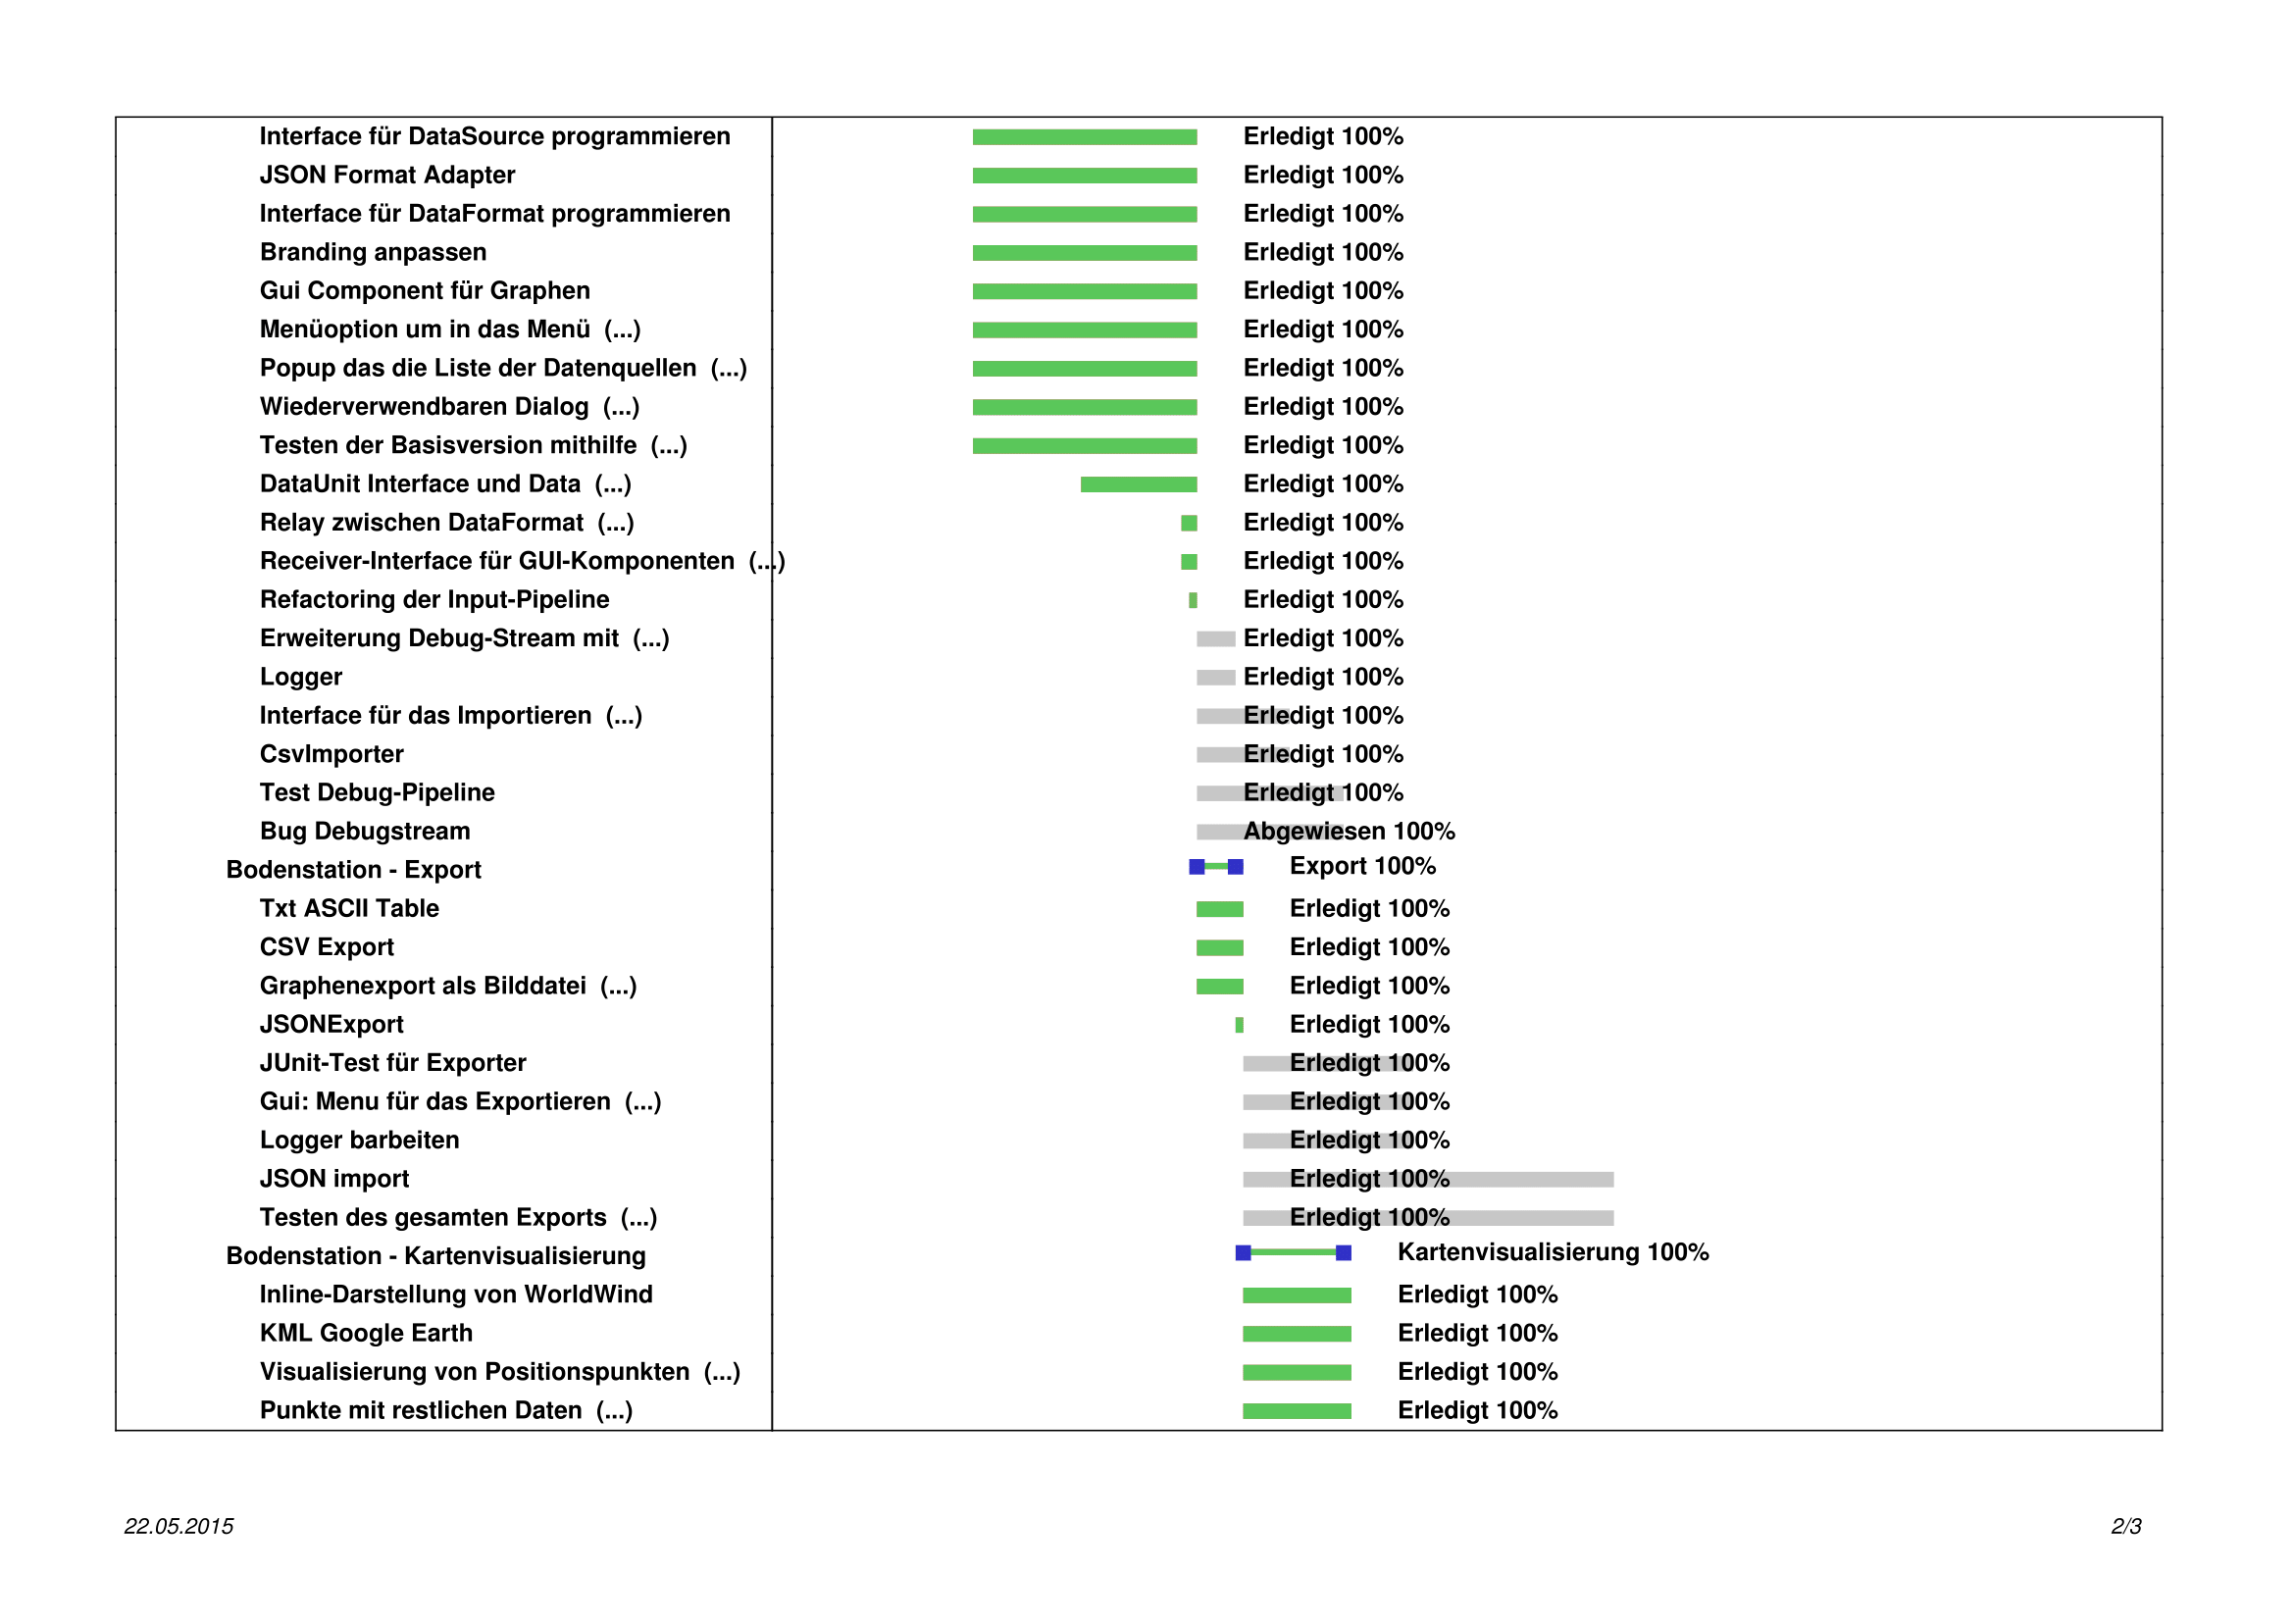
\includegraphics[trim = 30mm 50mm 45mm 40mm, clip,width=0.8\textwidth]{8_Anhang/bodenstation-gantt-2.png}
	\label{gantt_hardware_2}
\end{figure}
\vspace{-1,1cm}
\begin{figure}[H]
	\centering
	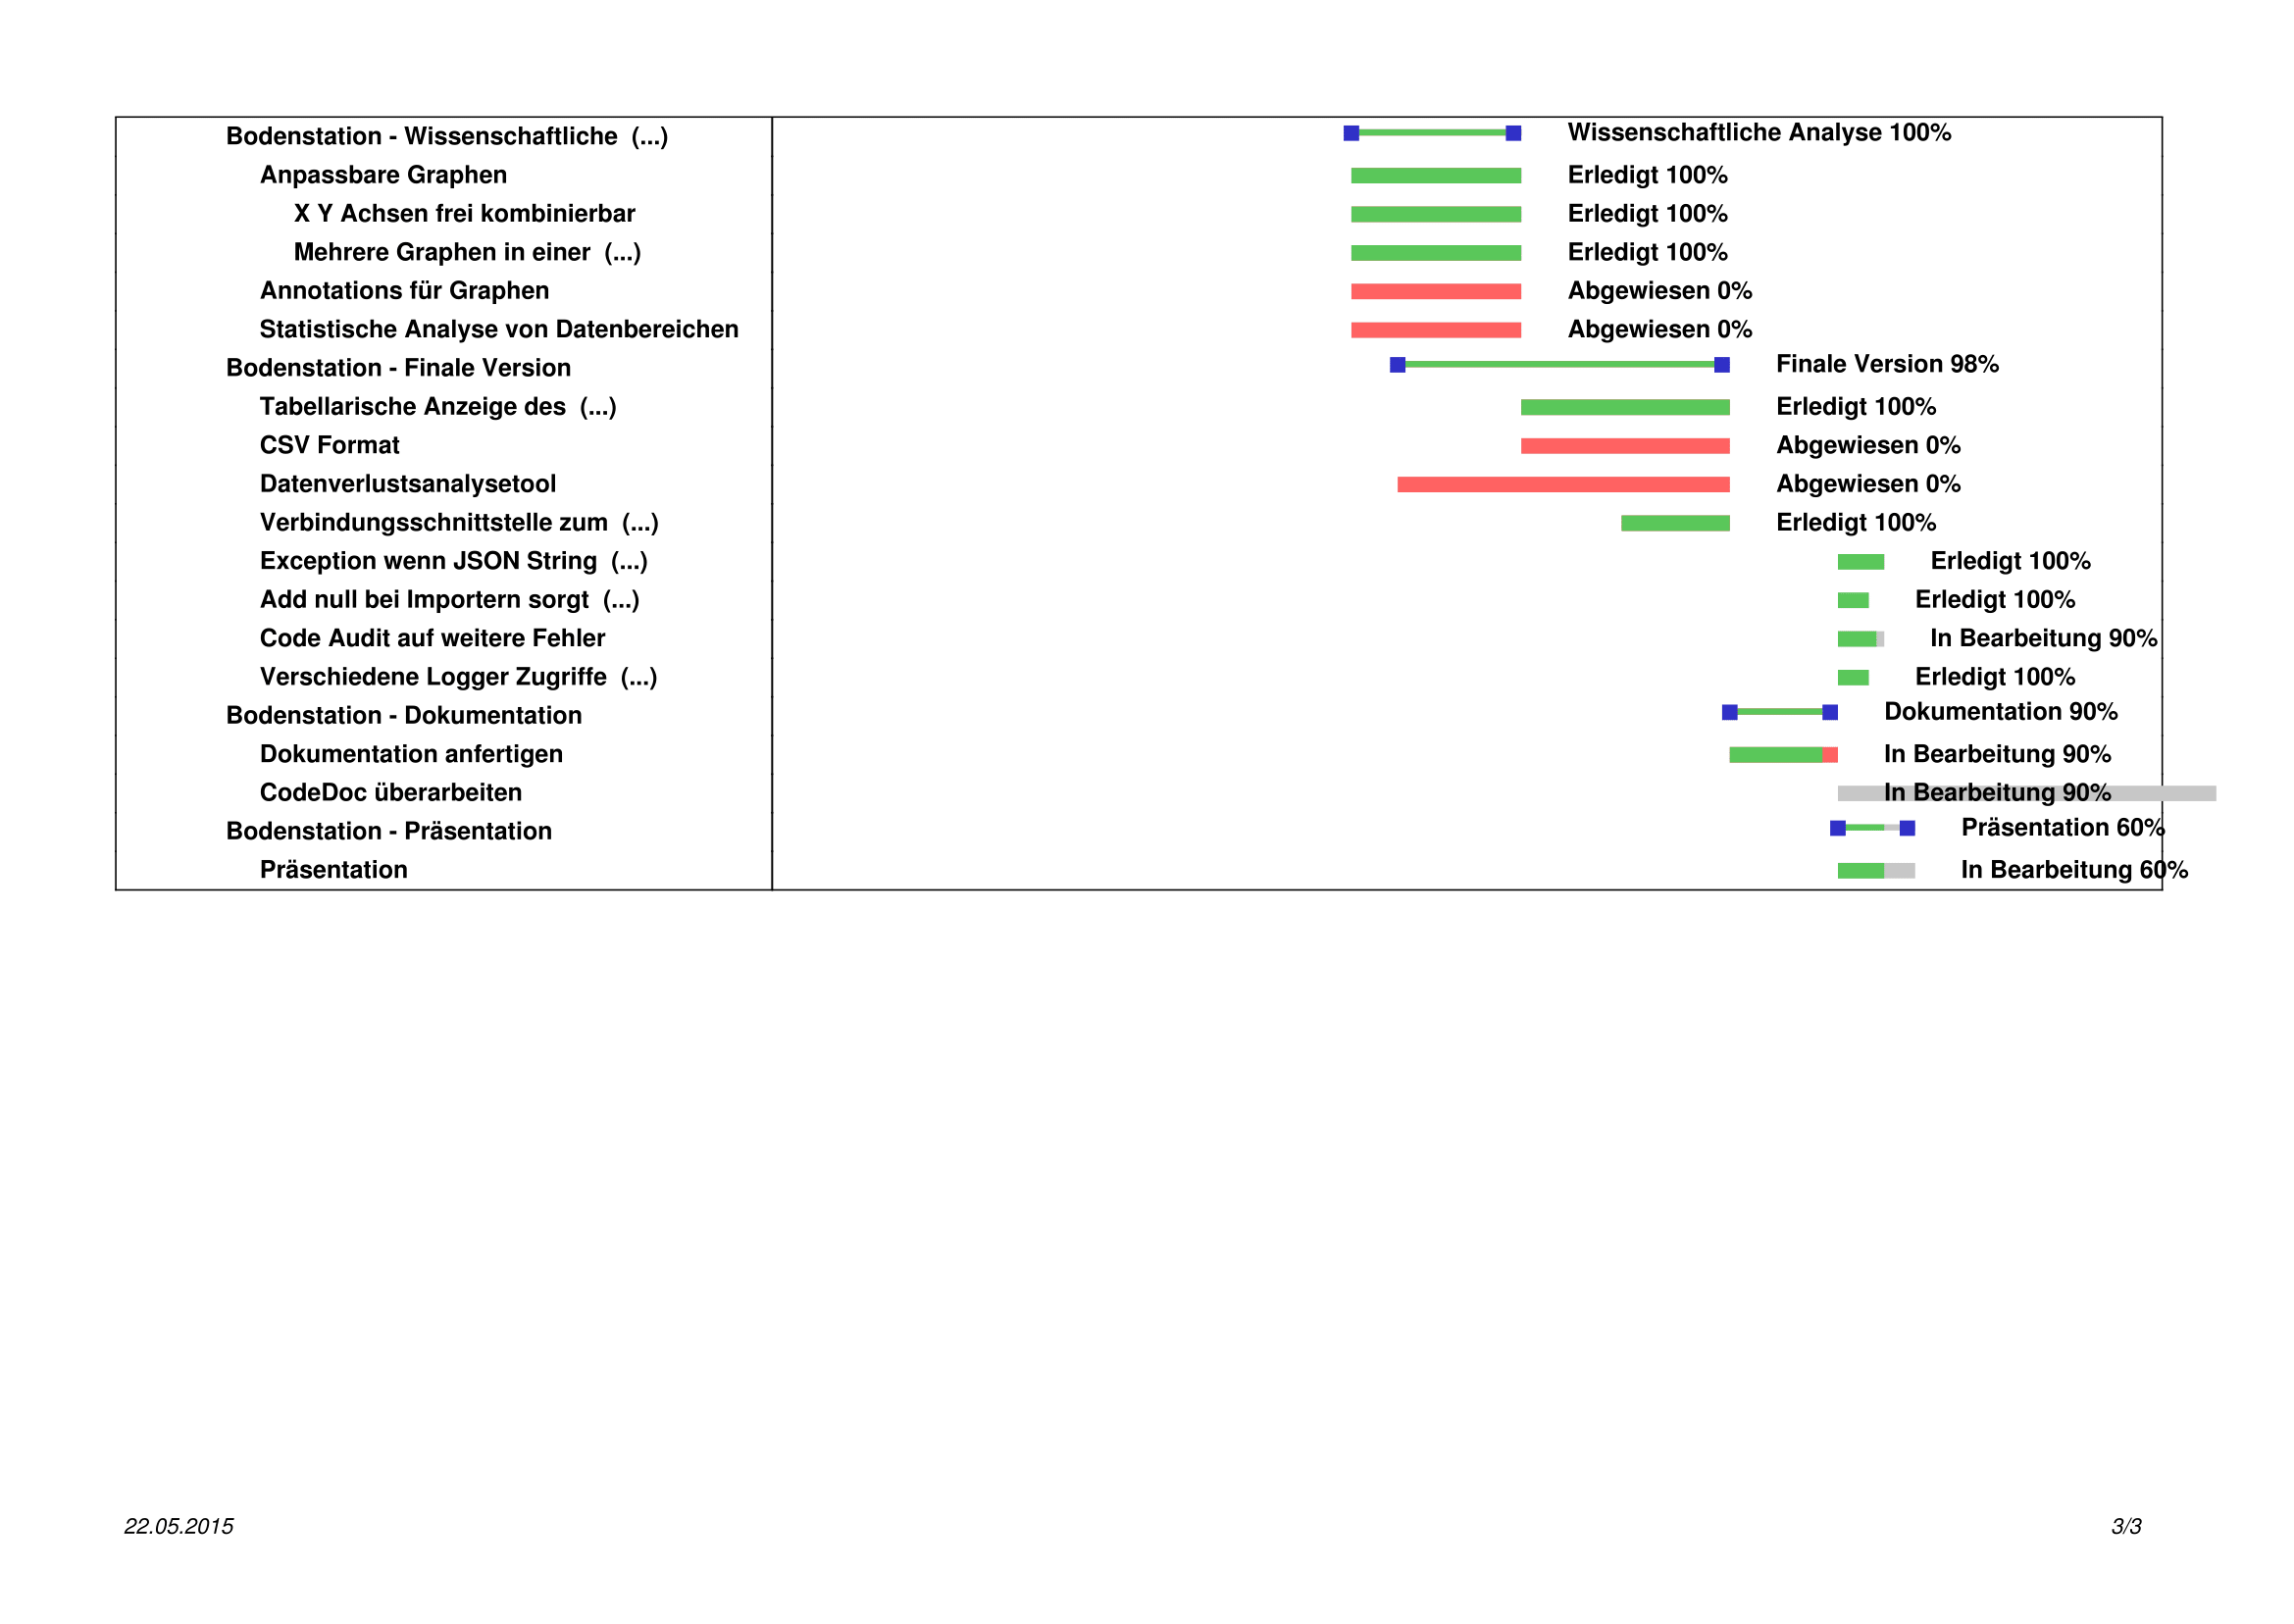
\includegraphics[trim = 30mm 200mm 45mm 40mm, clip,width=0.8\textwidth]{8_Anhang/bodenstation-gantt-3.png}
	\caption{Das GANTT-Diagramm der Bodenstation}
	\label{gantt_hardware_3}
\end{figure}
\newpage
\subsubsection {Android App-GANTT}
\begin{figure}[H]
	\centering
	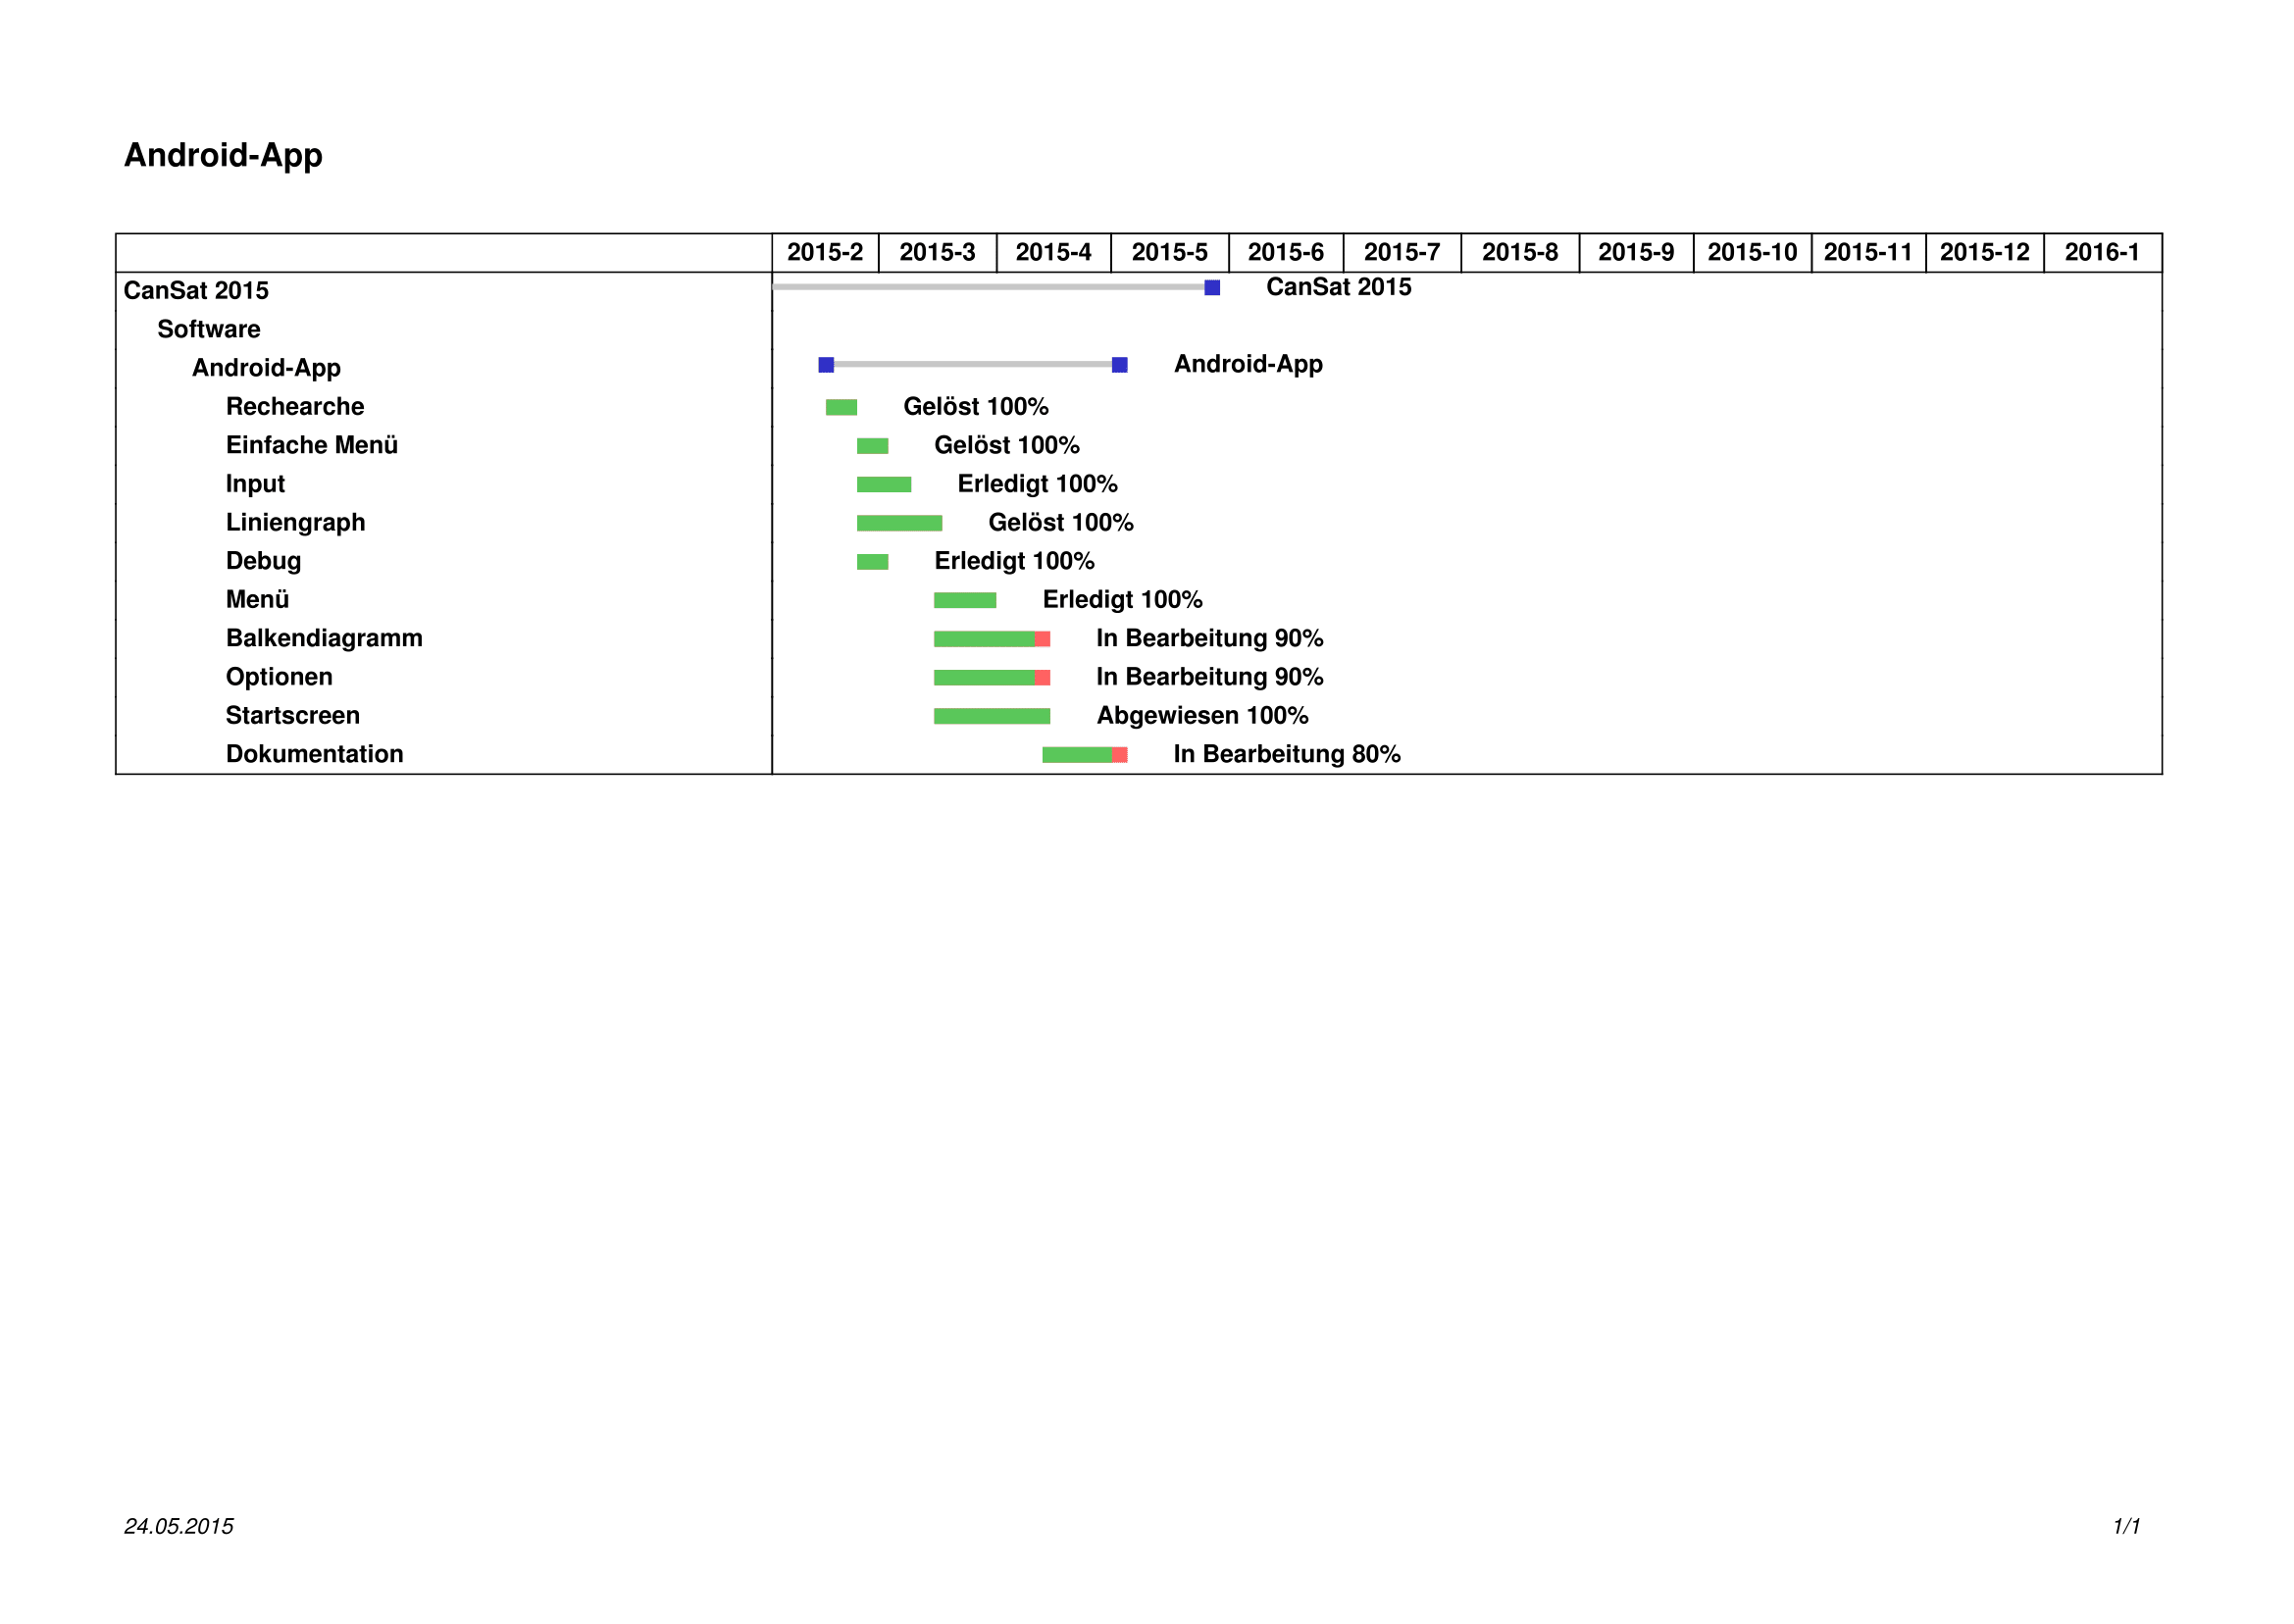
\includegraphics[trim = 30mm 200mm 45mm 40mm, clip,width=0.8\textwidth]{8_Anhang/android-app-gantt-1.png}
	\caption{Das GANTT-Diagramm der Bodenstation}
	\label{gantt_hardware_3}
\end{figure}
\newpage
\vspace{-2cm}
\subsection{Der CanSat}

\begin{figure}[H]
	\centering
	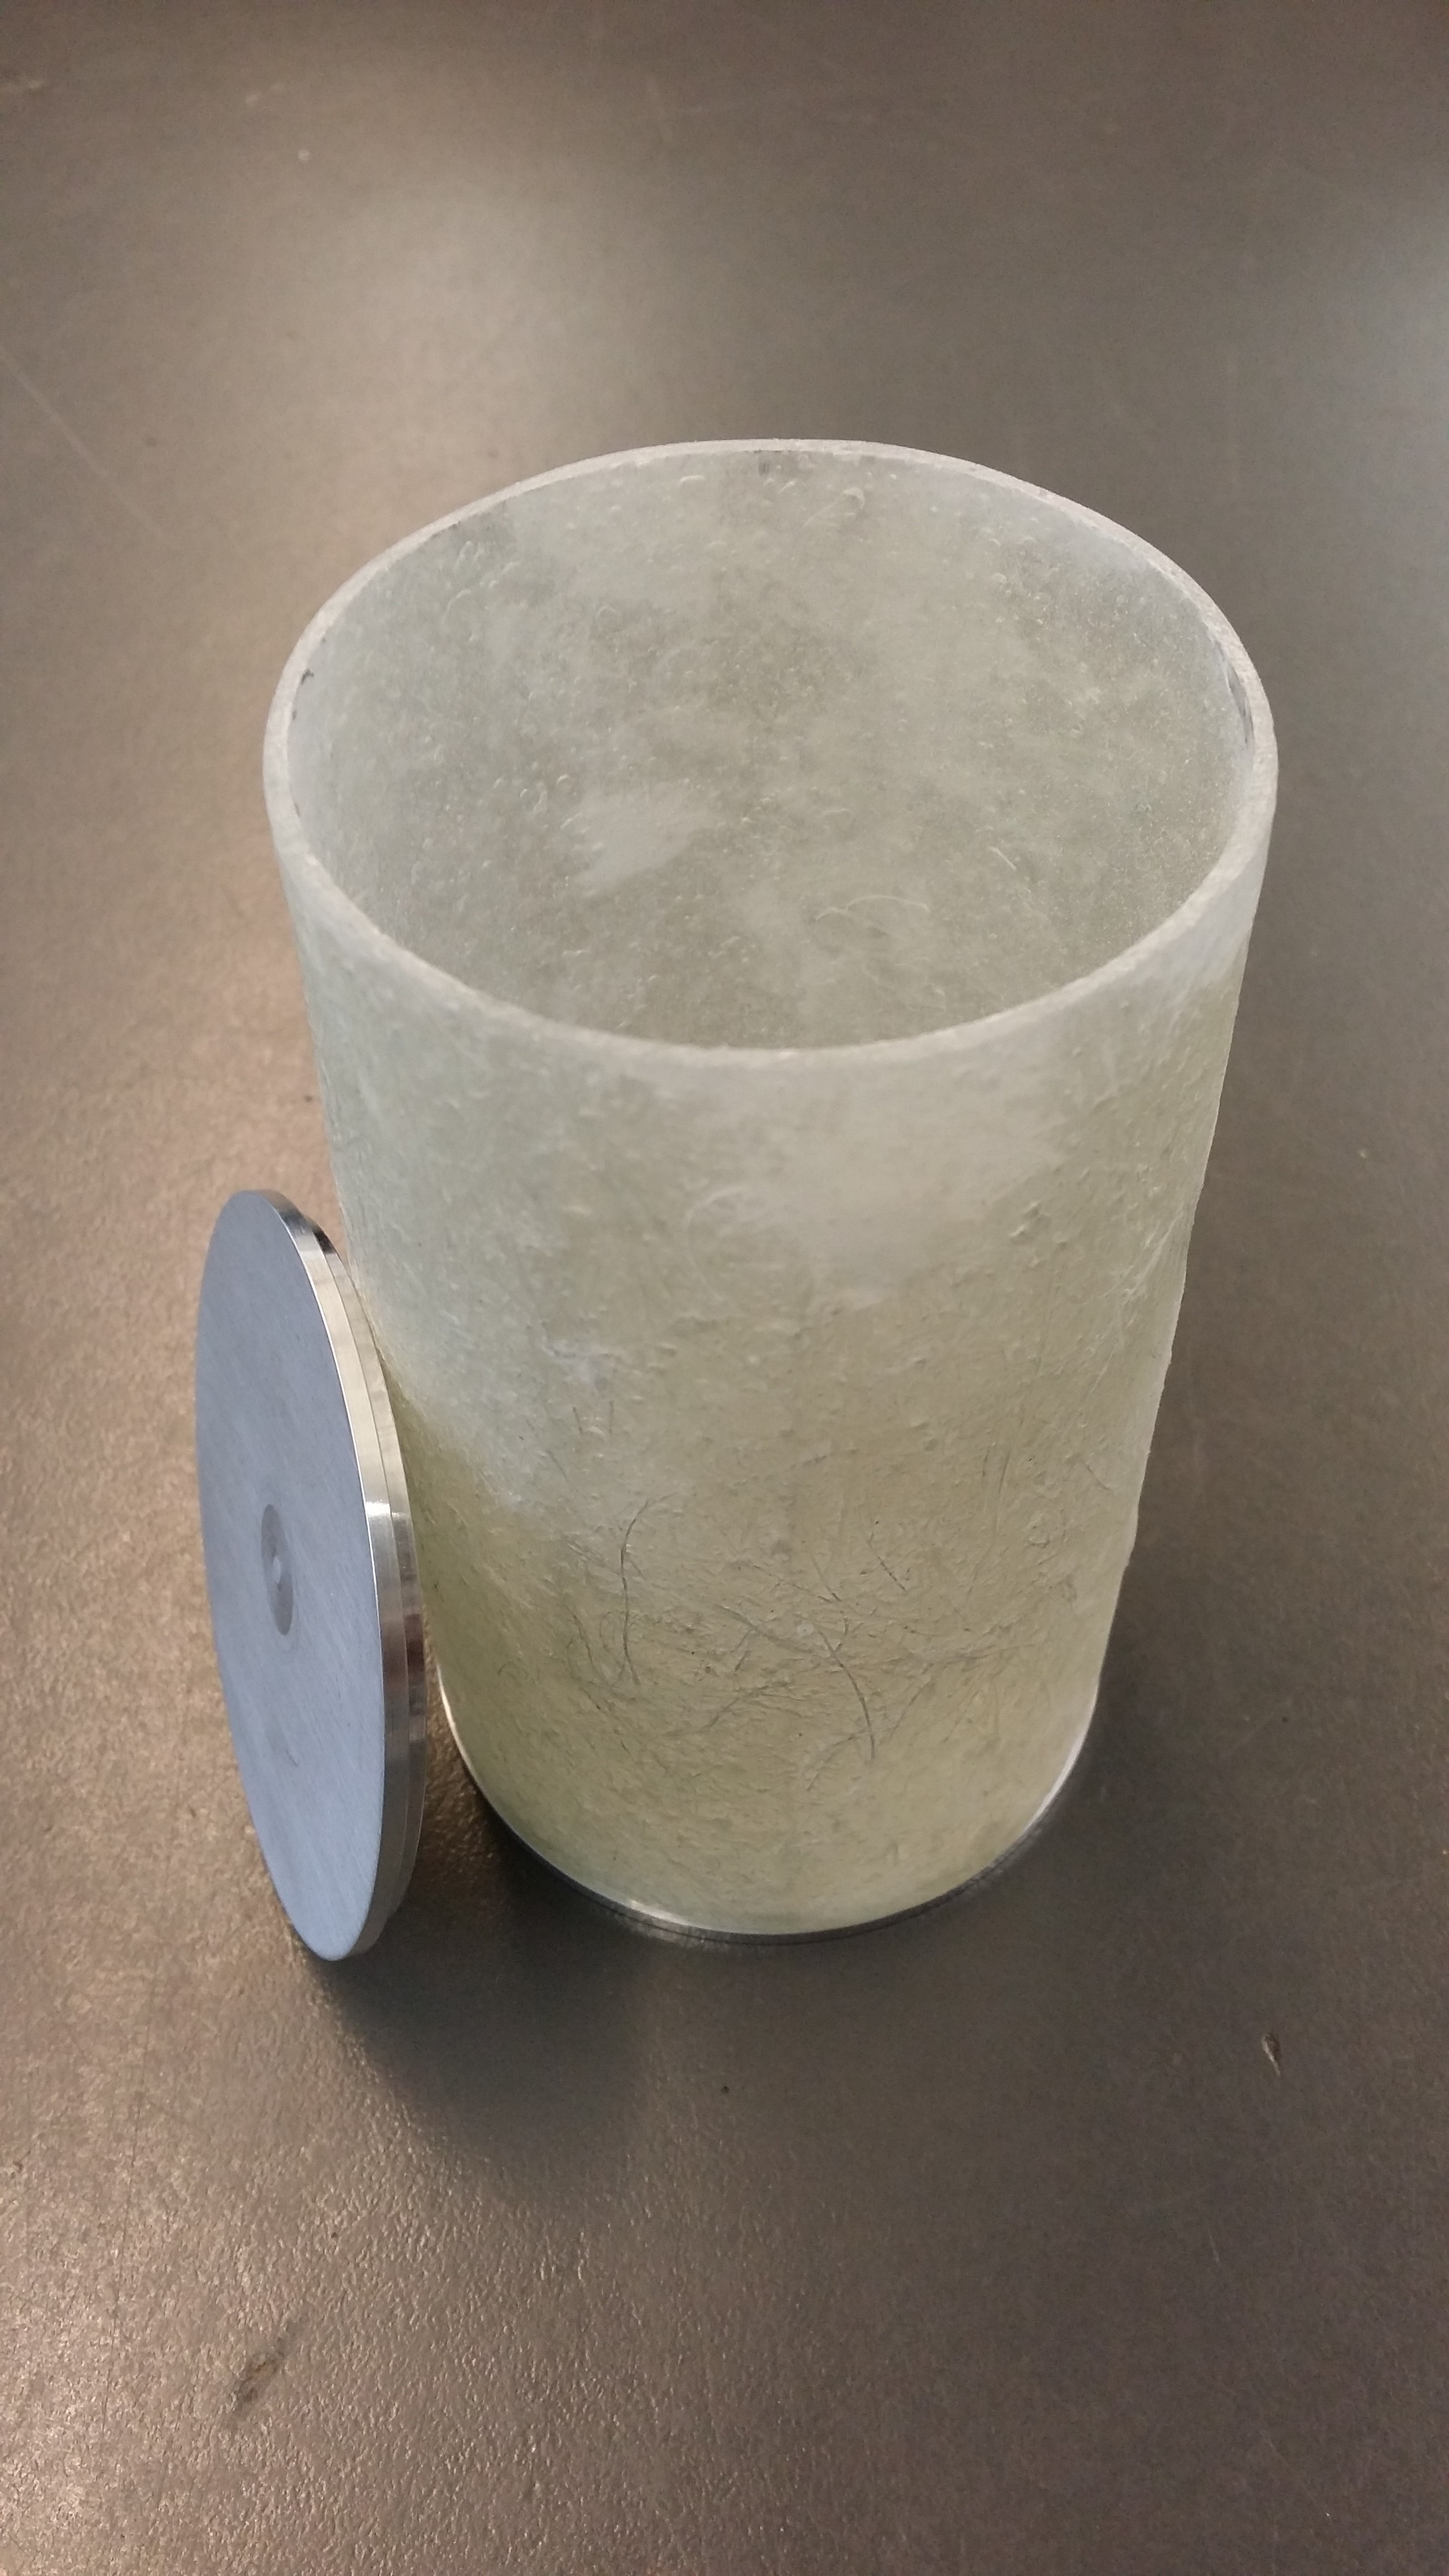
\includegraphics[trim = 11mm 335mm 20mm 210mm, clip, width=0.8\textwidth]{8_Anhang/dose.jpg}
	\caption{Die Hülle und ein Dosendeckel}
	\label{pic_dose}
\end{figure}

\begin{figure}[H]
	\centering
	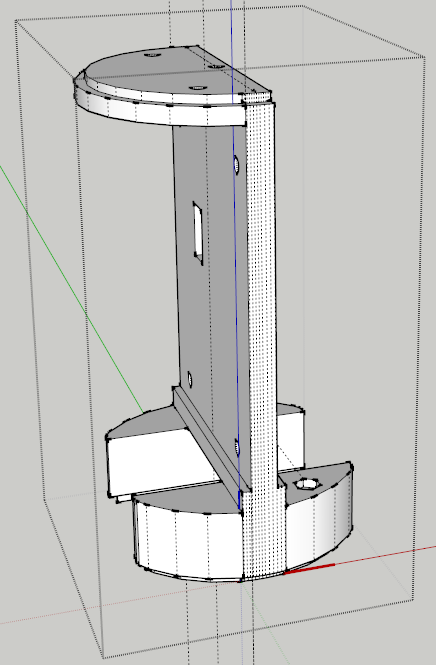
\includegraphics[ width=0.8\textwidth]{8_Anhang/Wand_3D.PNG}
	\caption{Screenshot der Zwischenwand aus Sketchup}
	\label{pic_wand_3d}
\end{figure}

\newpage

\begin{figure}[h] 
      \centering 
      \includemovie[ 
        poster,controls,
       3Djscript=2_Beschreibung_des_CANSAT/Encompass.js
      ]{0.8\textwidth}{15cm}{2_Beschreibung_des_CANSAT/CanSat_2015.u3d} 
      \caption{Der Satellit (Diese Zeichnung ist möglicherweiße nicht sichtbar, da es eine 3D Zeichnung ist. Bitte verwenden Sie den \href{https://get.adobe.com/reader/?loc=de}{Adobe Acrobat Reader})}\label{pic_3d} 
\end{figure} 

\newpage

\begin{figure}[H]
	\centering
	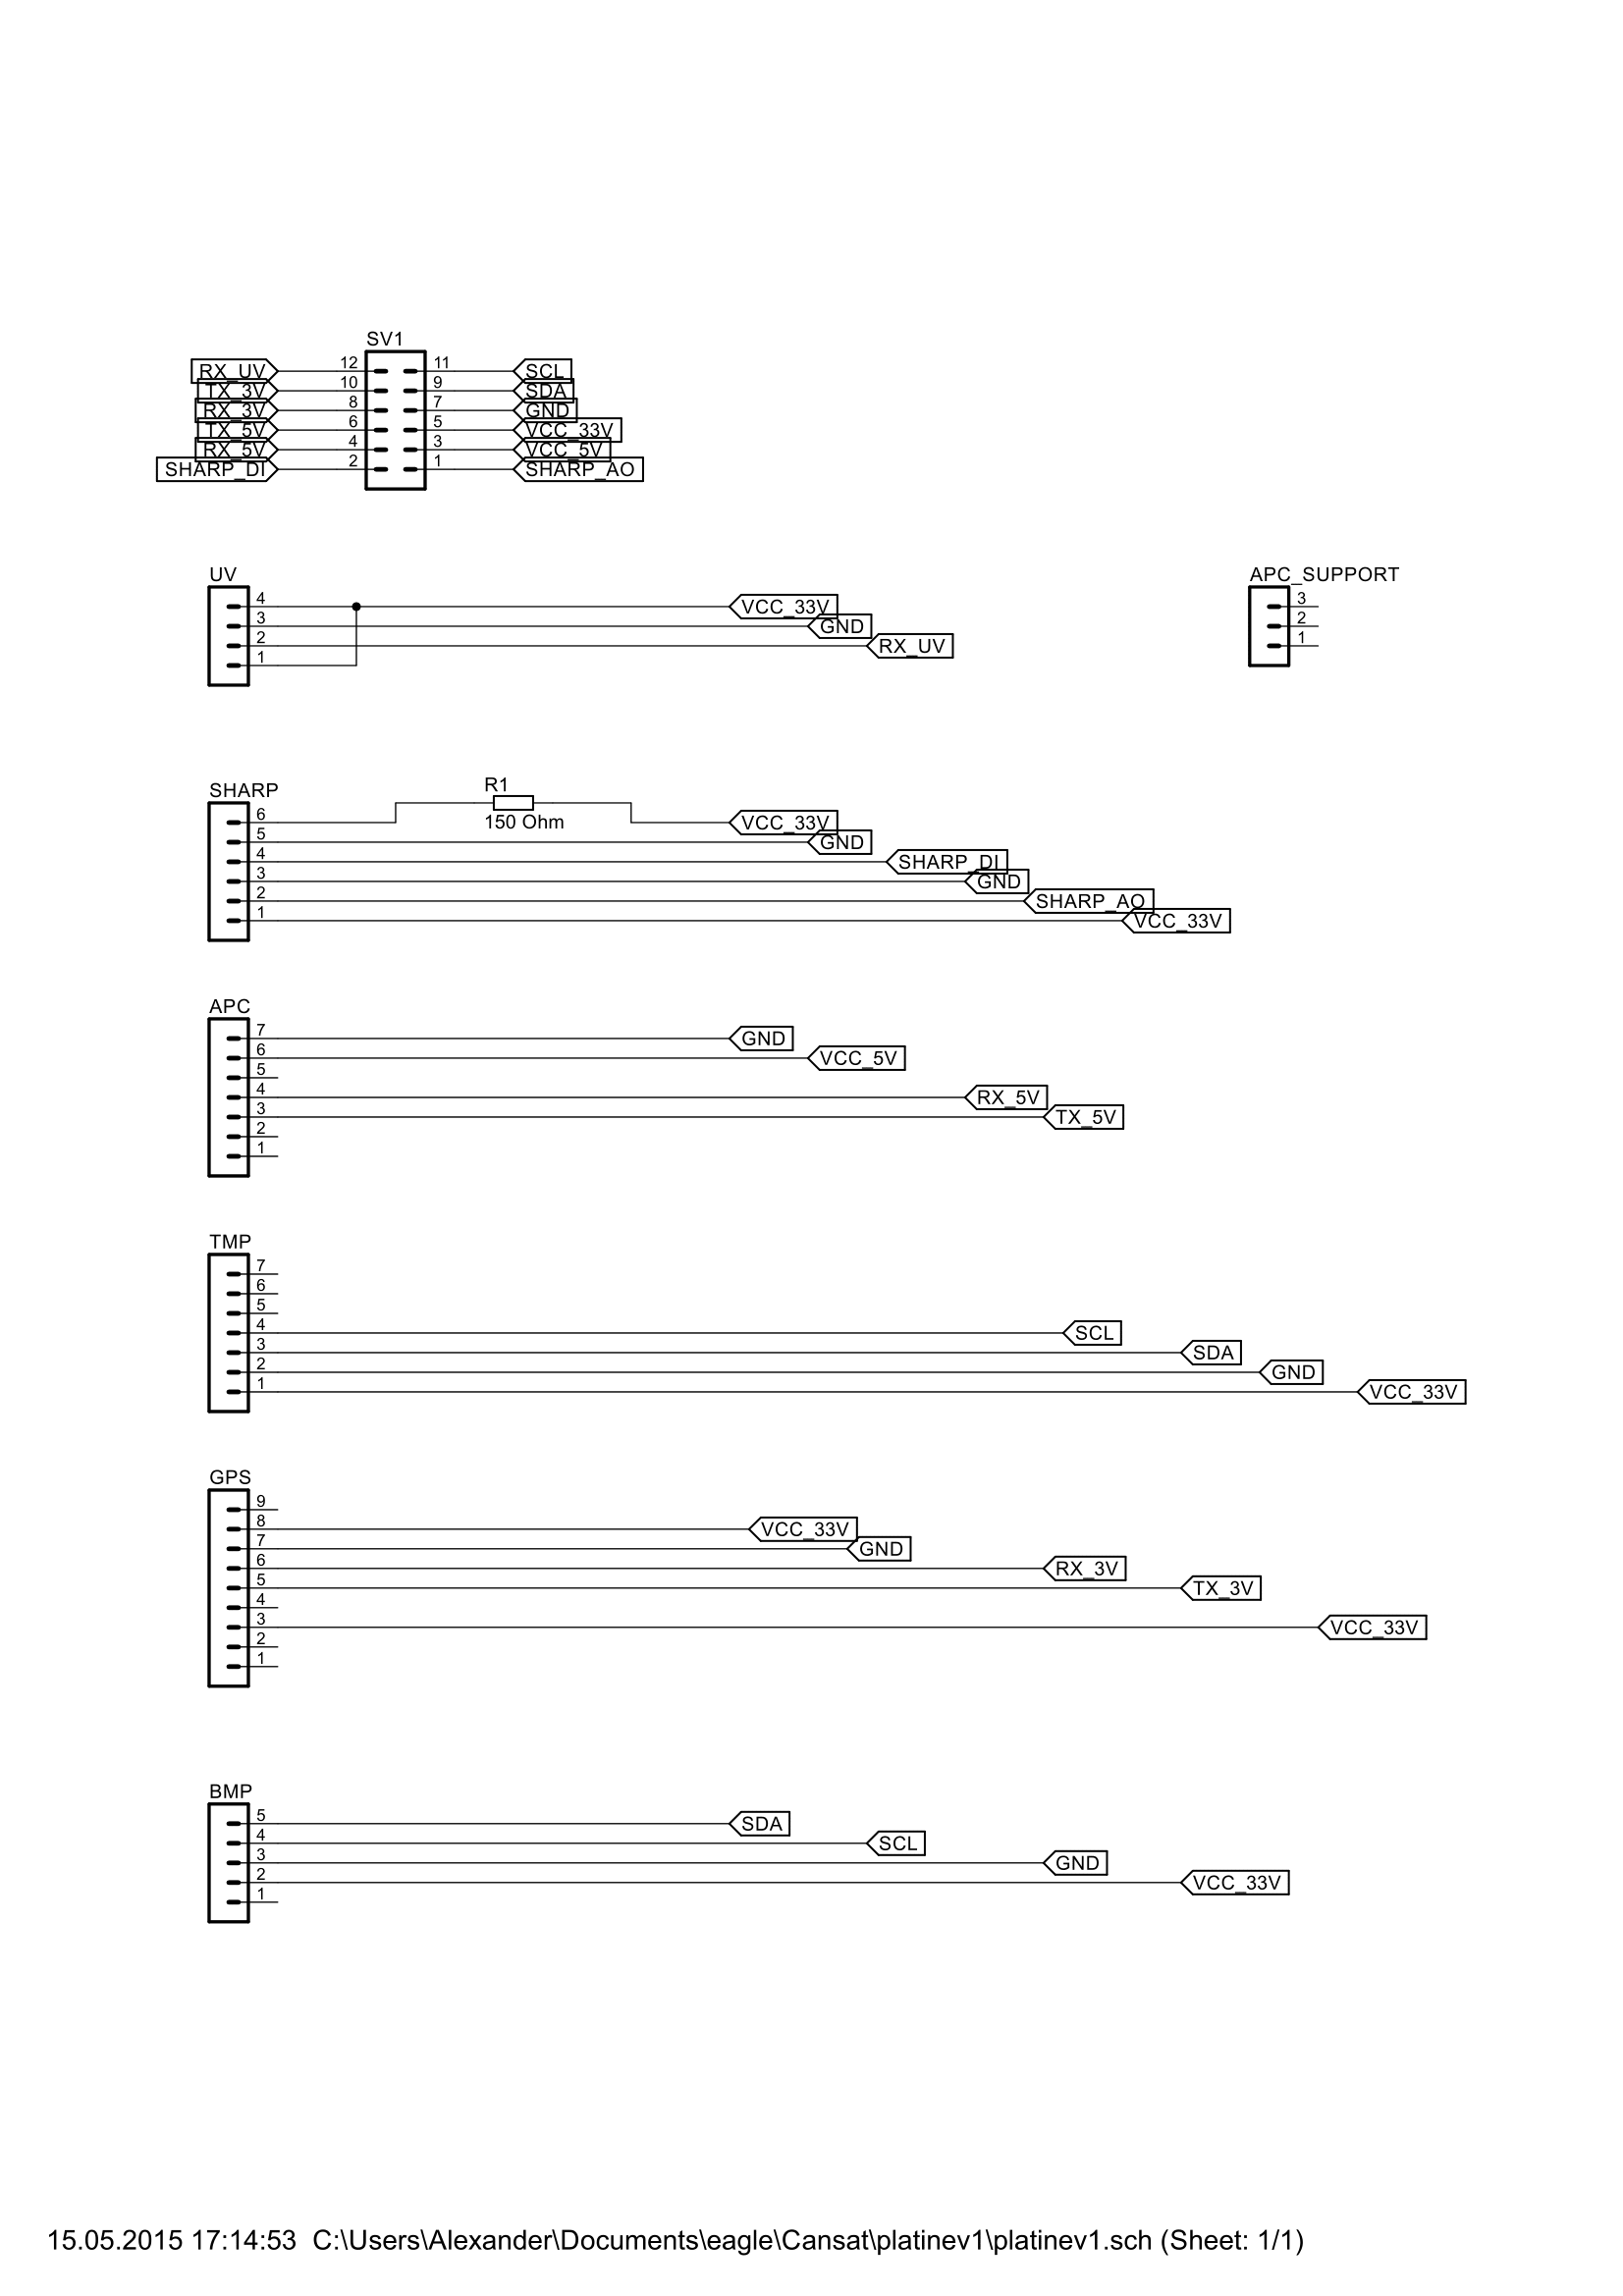
\includegraphics[trim = 60mm 100mm 55mm 100mm, clip, width=0.8\textwidth]{8_Anhang/Schaltplanv1.png}
	\caption{Der Schaltplan der Sensorik Platine}
	\label{pic_schaltplan}
\end{figure}

\newpage

\begin{figure}[H]
	\centering
	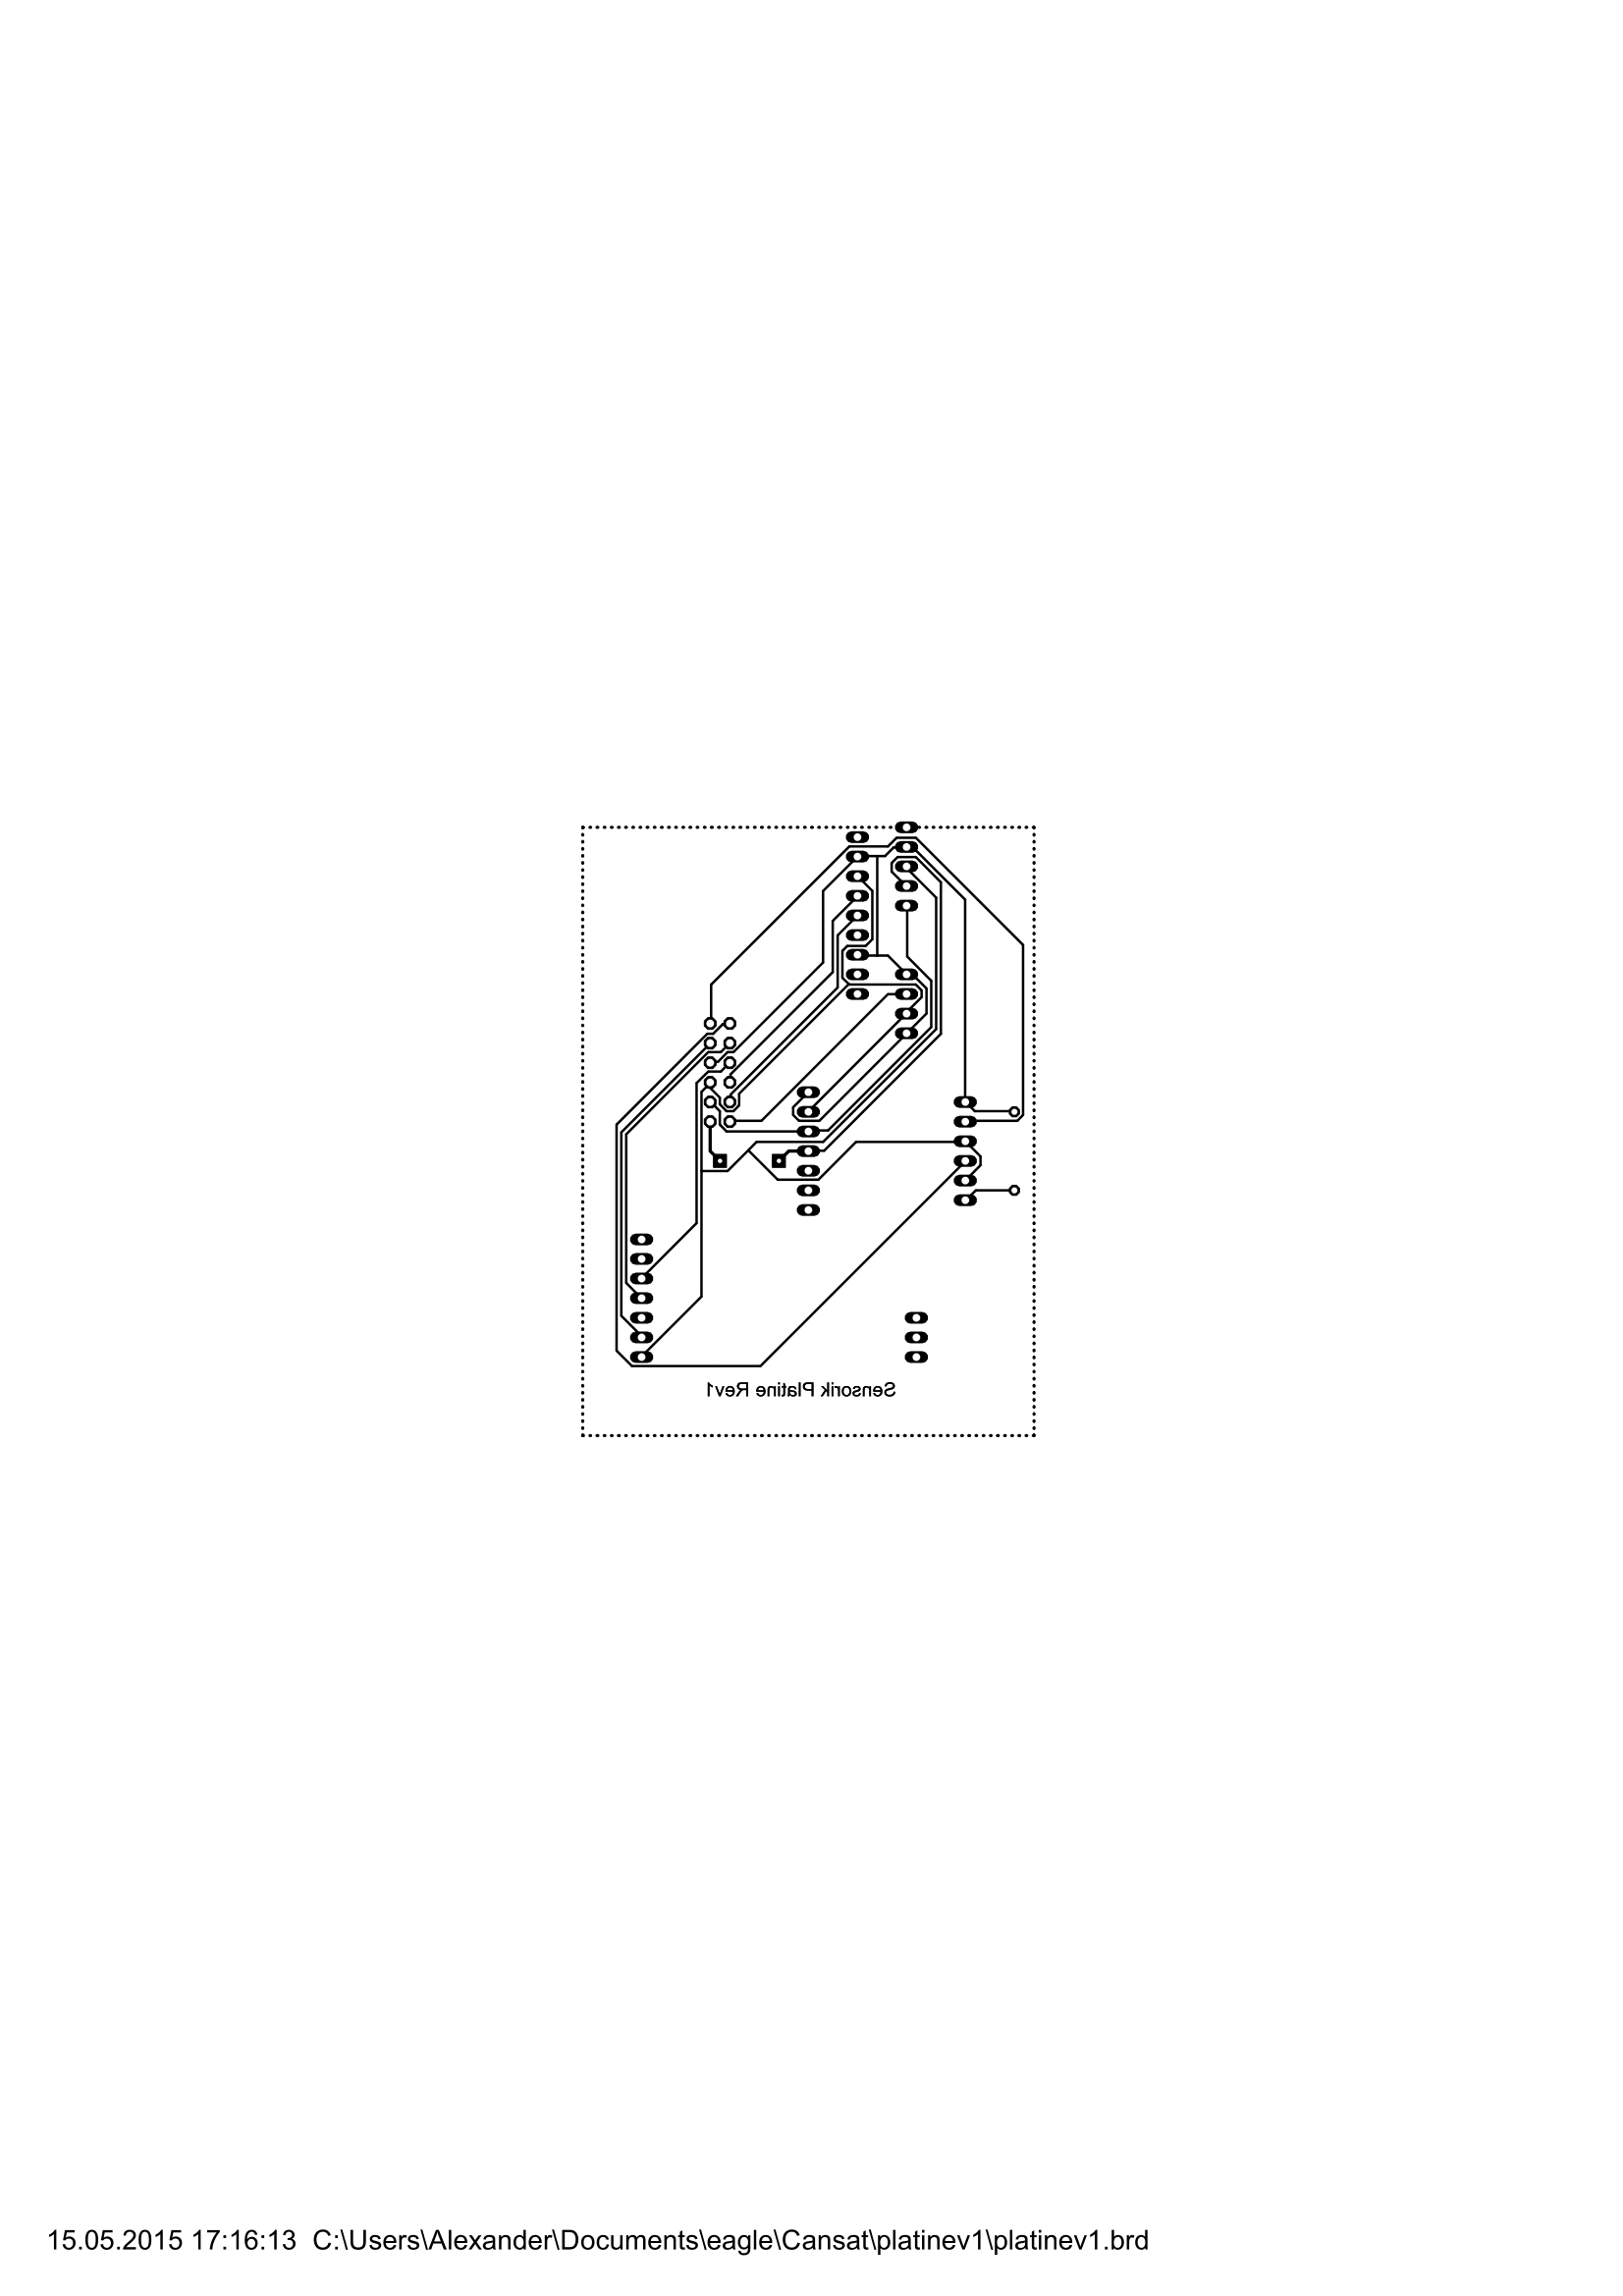
\includegraphics[trim = 200mm 300mm 200mm 280mm, clip,width=0.8\textwidth]{8_Anhang/Layoutv1.png}
	\caption{Das Layout der Sensorik Platine}
	\label{pic_layout}
\end{figure}

\newpage

\begin{figure}[H]
	\centering
	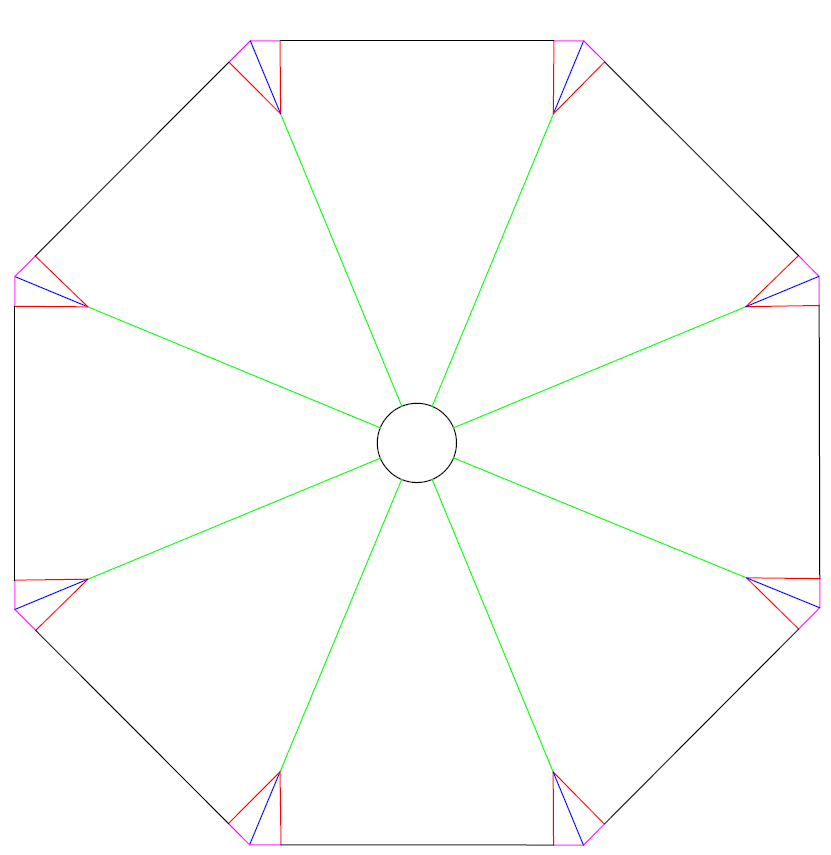
\includegraphics[ width=0.8\textwidth]{8_Anhang/fallschirmSkizze.PNG}
	\caption{Skizze des Fallschirms}
	\label{pic_fallschrimskizze}
\end{figure}

\newpage

\subsection{Bodenstationsarchitektur}
\begin{figure}[H]
	\centering
	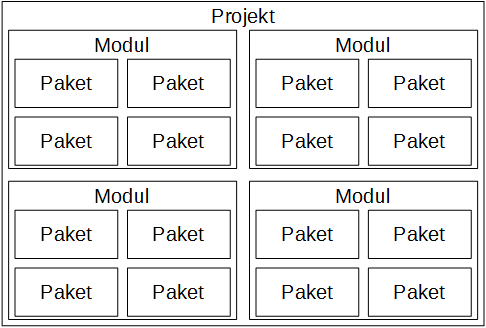
\includegraphics[width=0.8\textwidth]{3_Beschreibung_der_Bodenstation/NBP_Modularchitektur.png}
	\caption{Modularchitektur von Netbeans Platform}
	\label{nbp_modularchitektur}
\end{figure}

\begin{figure}[H]
	\centering
	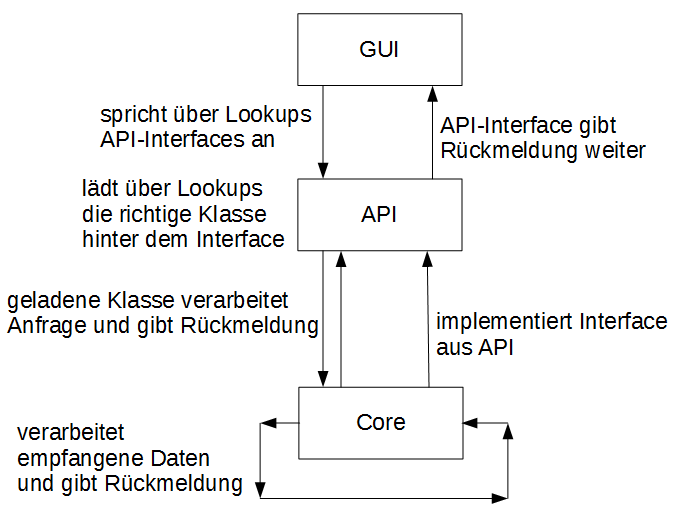
\includegraphics[width=0.8\textwidth]{3_Beschreibung_der_Bodenstation/Bodenstation_Modularchitektur.png}
	\caption{Modularchitektur der Bodenstation}
	\label{station_modularchitektur}
\end{figure}
\vspace{-5cm}

\newpage

\begin{figure}[H]
	\centering
	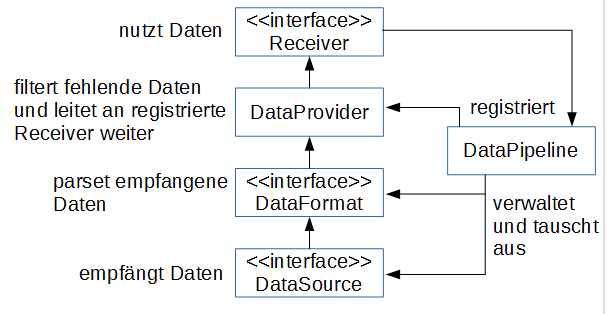
\includegraphics[width=0.8\textwidth]{3_Beschreibung_der_Bodenstation/Input-Pipeline_Architektur.png}
	\caption{Architektur der Input-Pipeline}
	\label{inputpipeline}
\end{figure}

\newpage
\subsection{Protokolle}
Auf den nachfolgenden Seiten finden sich Protokolle diverser Meetings. Diese Protokolle wurden mal mit mehr, und mal mit weniger Mühe und Aufwand angefertigt. Uns war lediglich wichtig, dass es Protokolle gibt, an denen wir unsere Arbeit belegen können, und an denen bereits getroffene Entscheidungen nachvollzogen werden können.

\includepdf[pages=-]{8_Anhang/Protokolle/140625_Meeting_Protokoll}%

\newpage
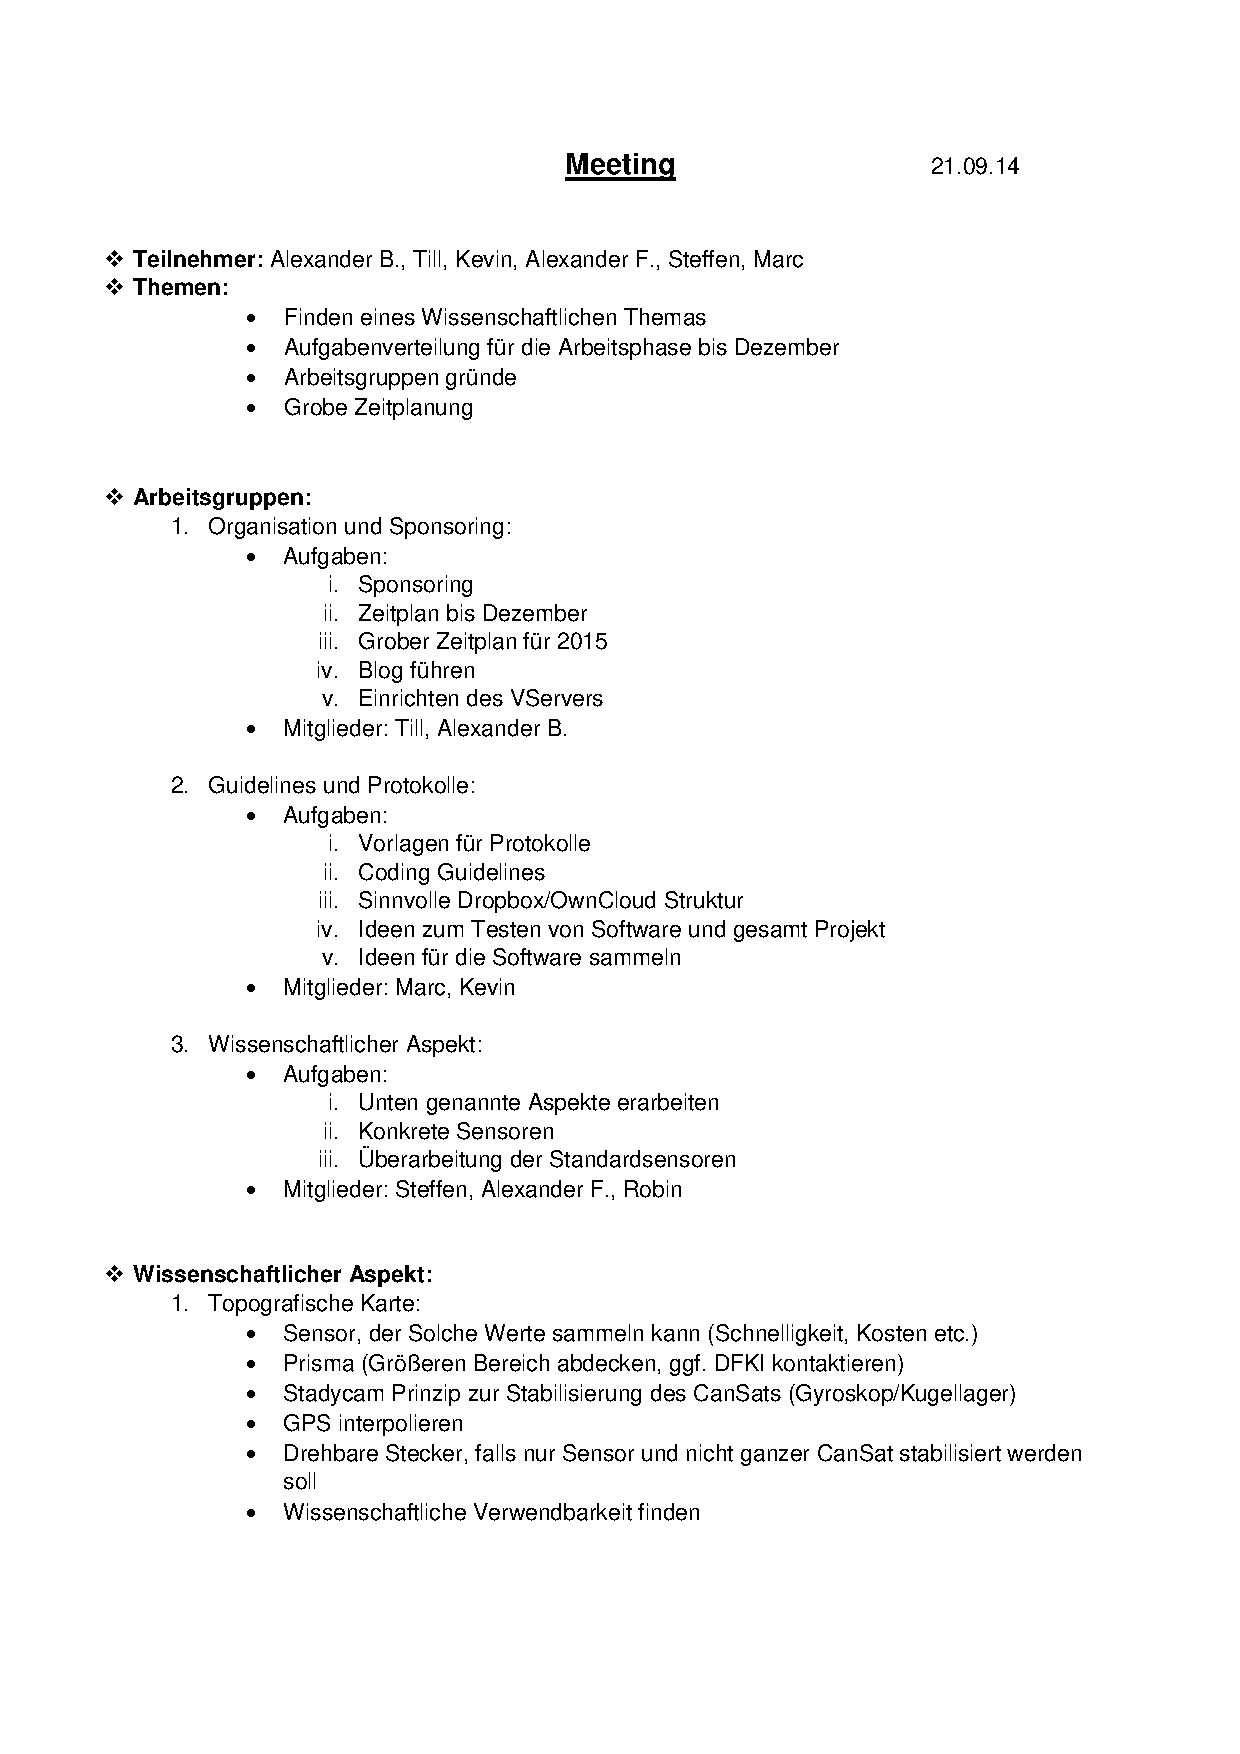
\includepdf[pages=-]{8_Anhang/Protokolle/140921_Meeting_Protokoll}%

\newpage
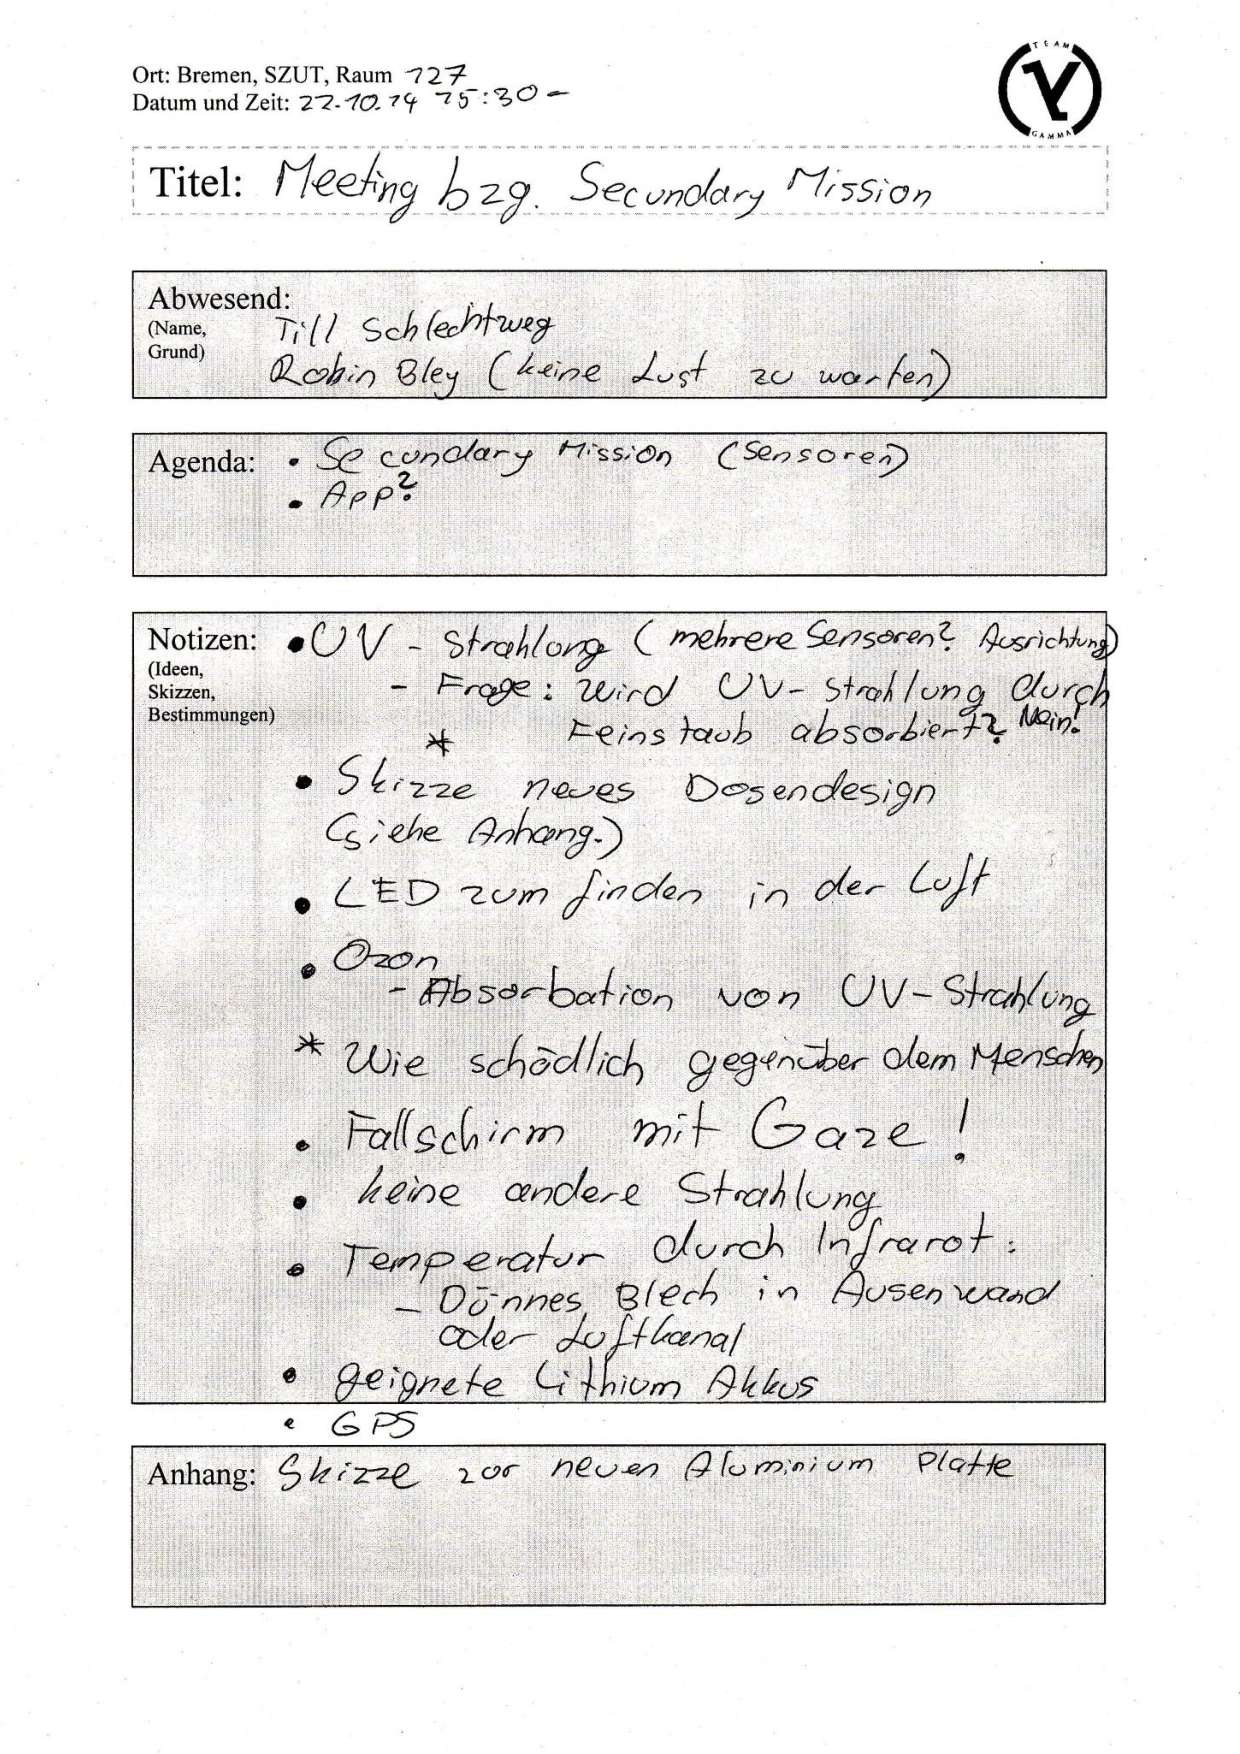
\includepdf[pages=-]{8_Anhang/Protokolle/141022_Meeting_Protokoll}%

\newpage
\begin{figure}[H]
	\centering
	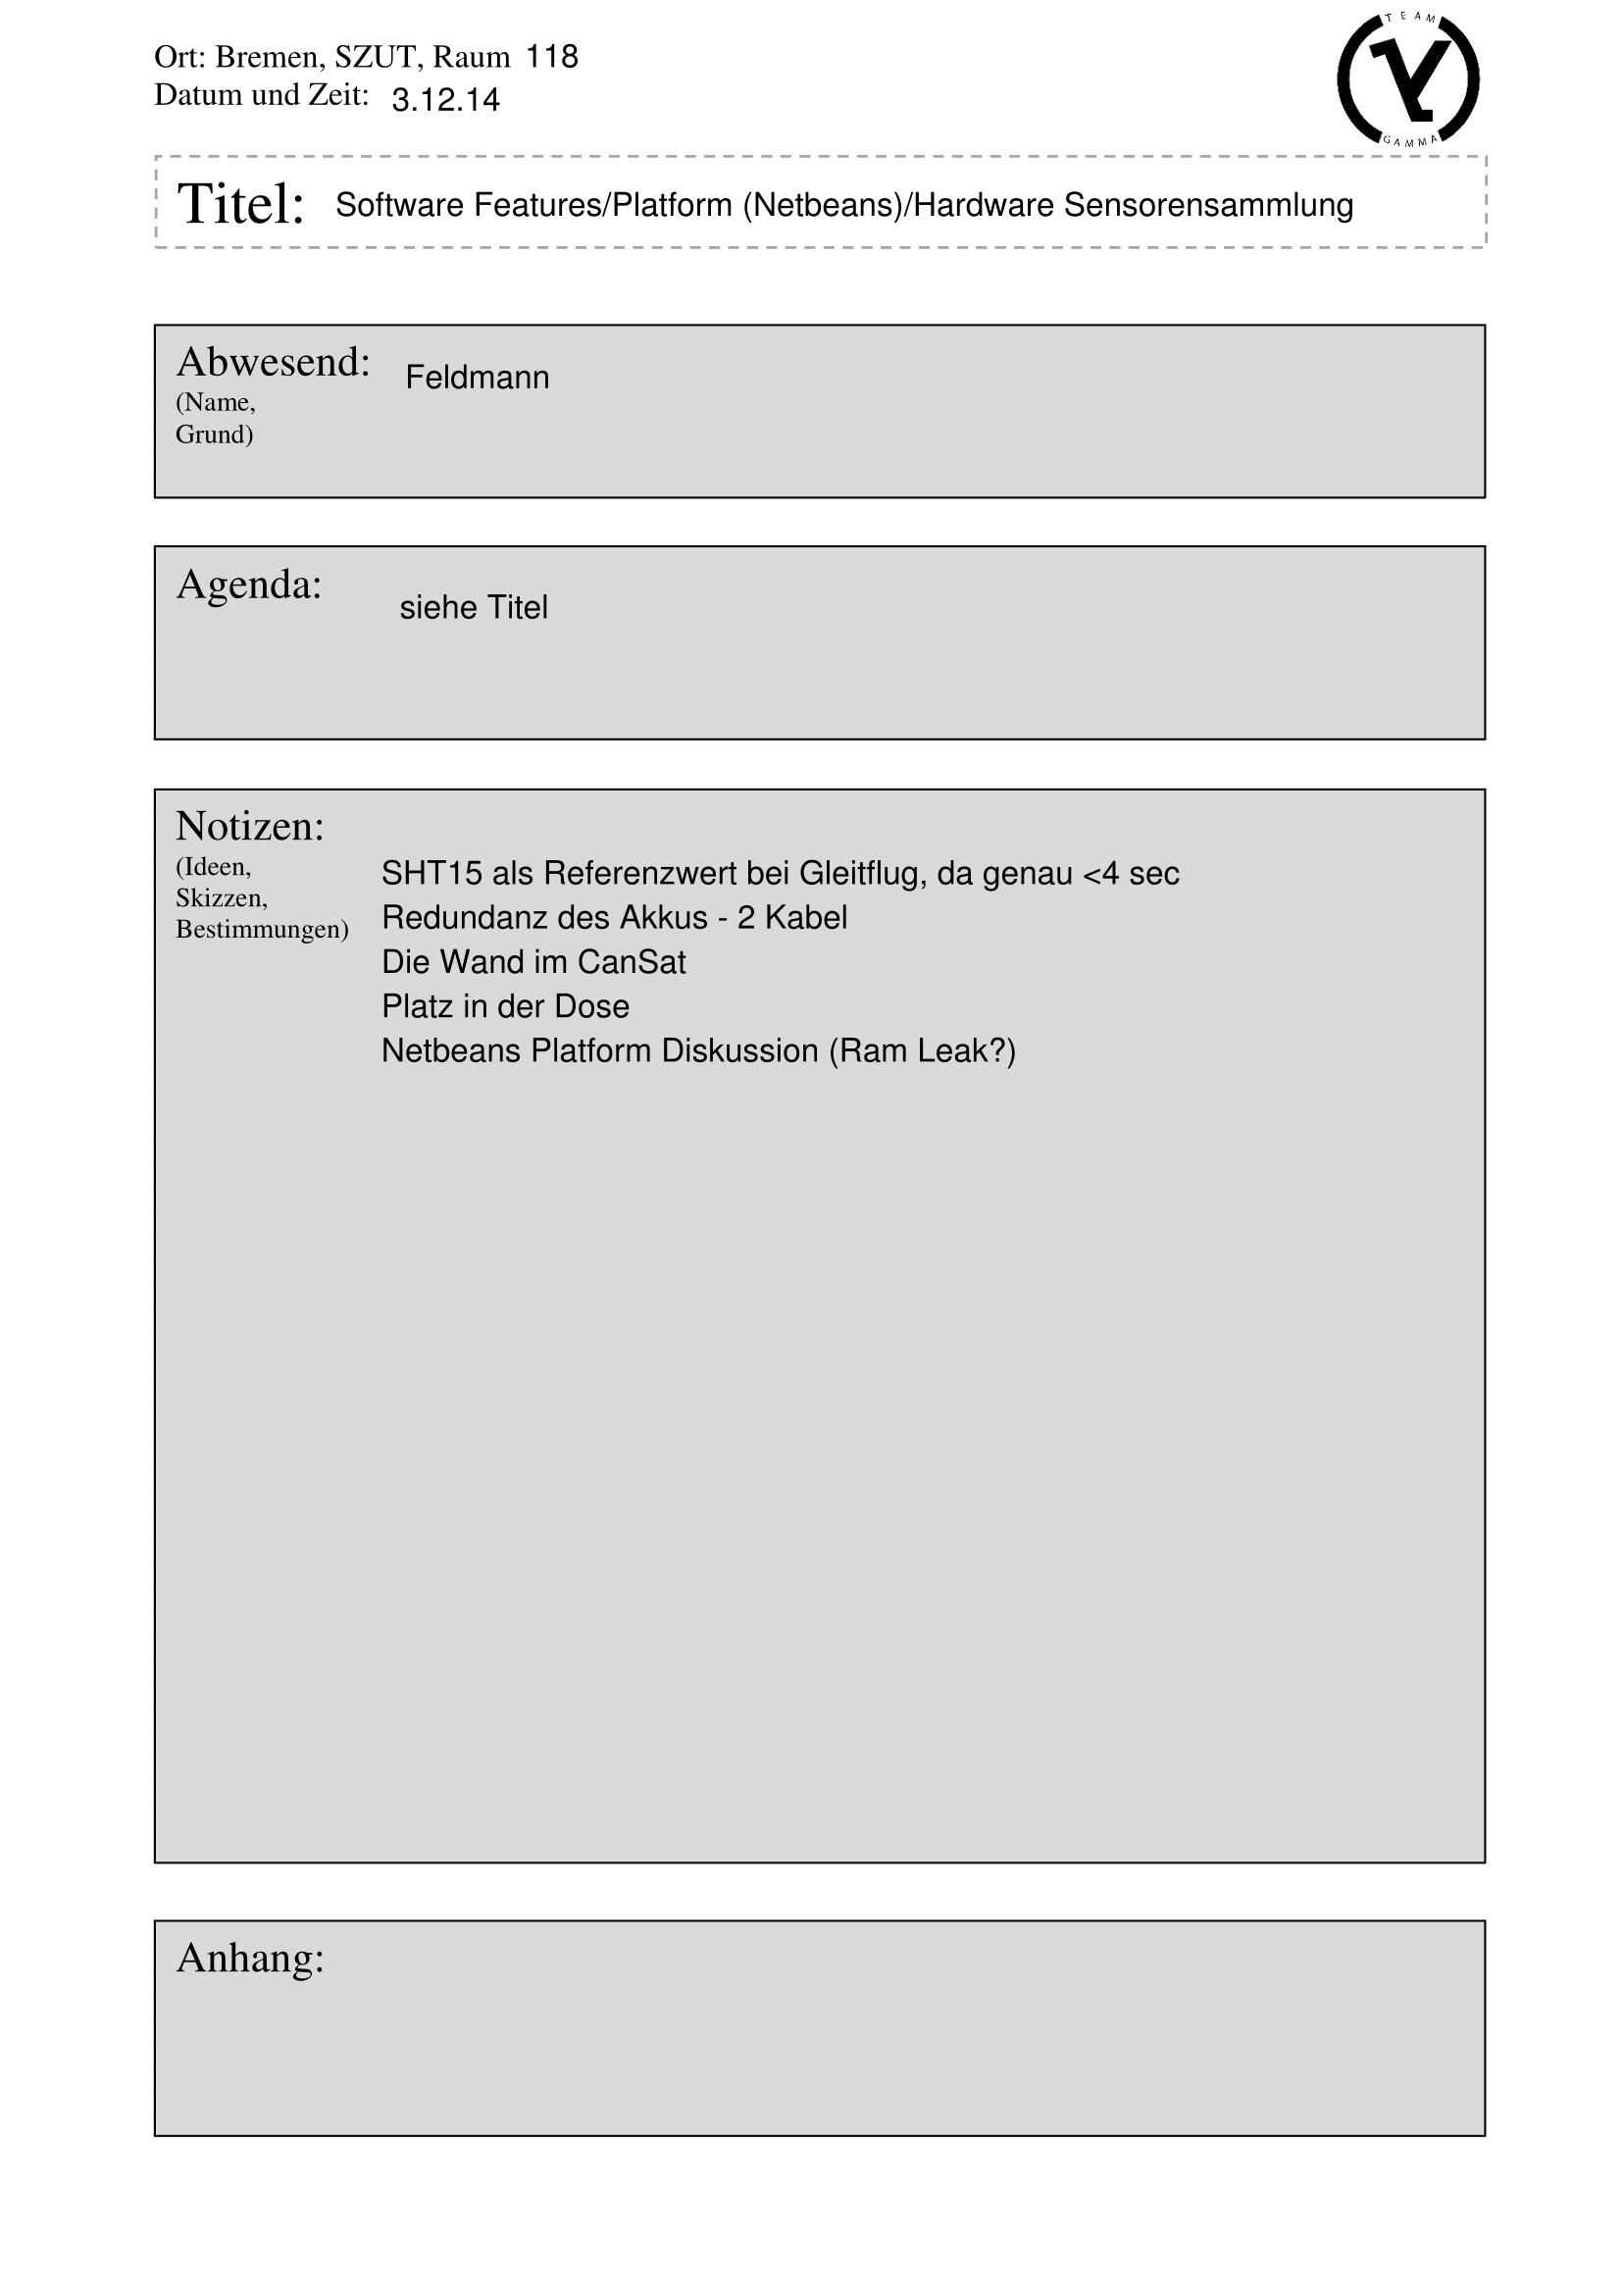
\includegraphics[width=0.8\textwidth]{8_Anhang/Protokolle/141203_Meeting_Protokoll.png}%
	\label{pic_protokoll_140203}
\end{figure}

\newpage
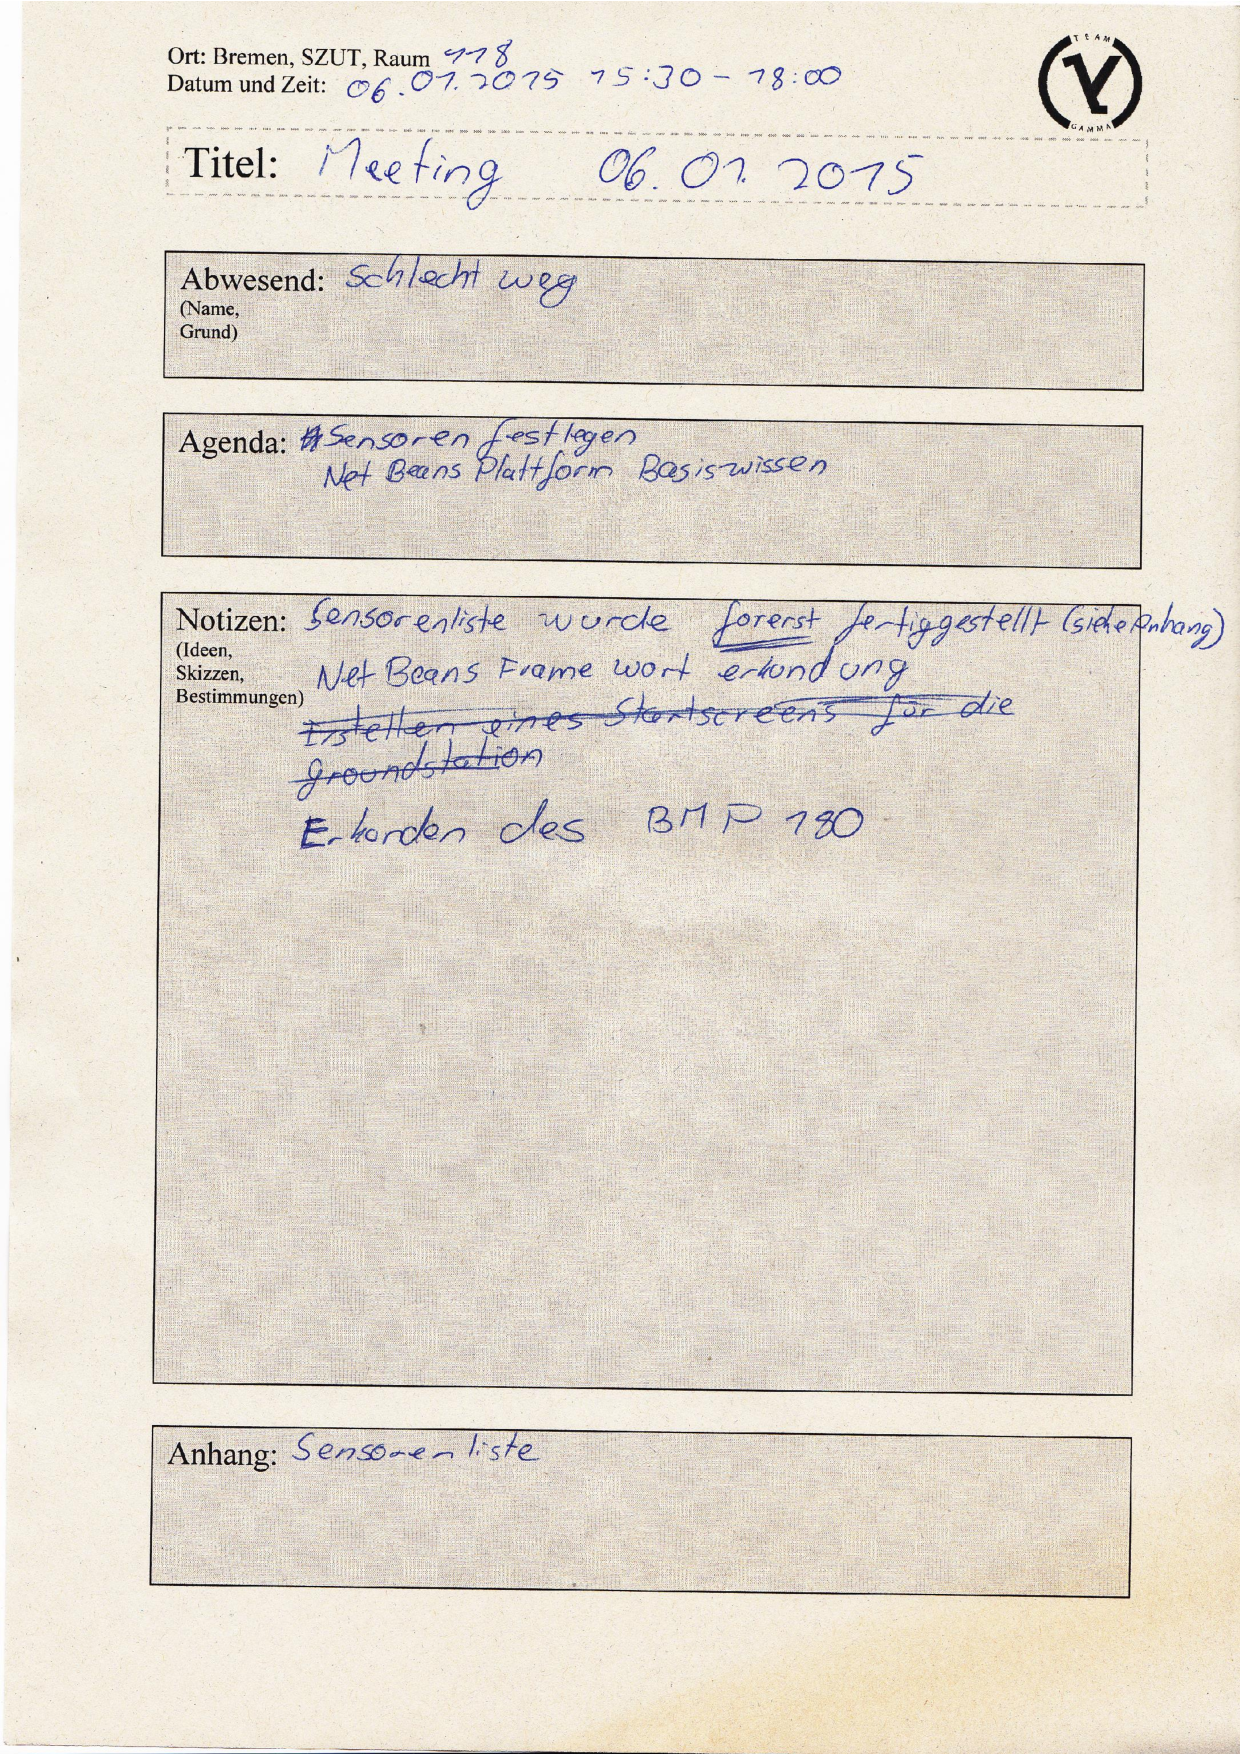
\includepdf{8_Anhang/Protokolle/150106_Meeting_Protokoll}%
\newpage

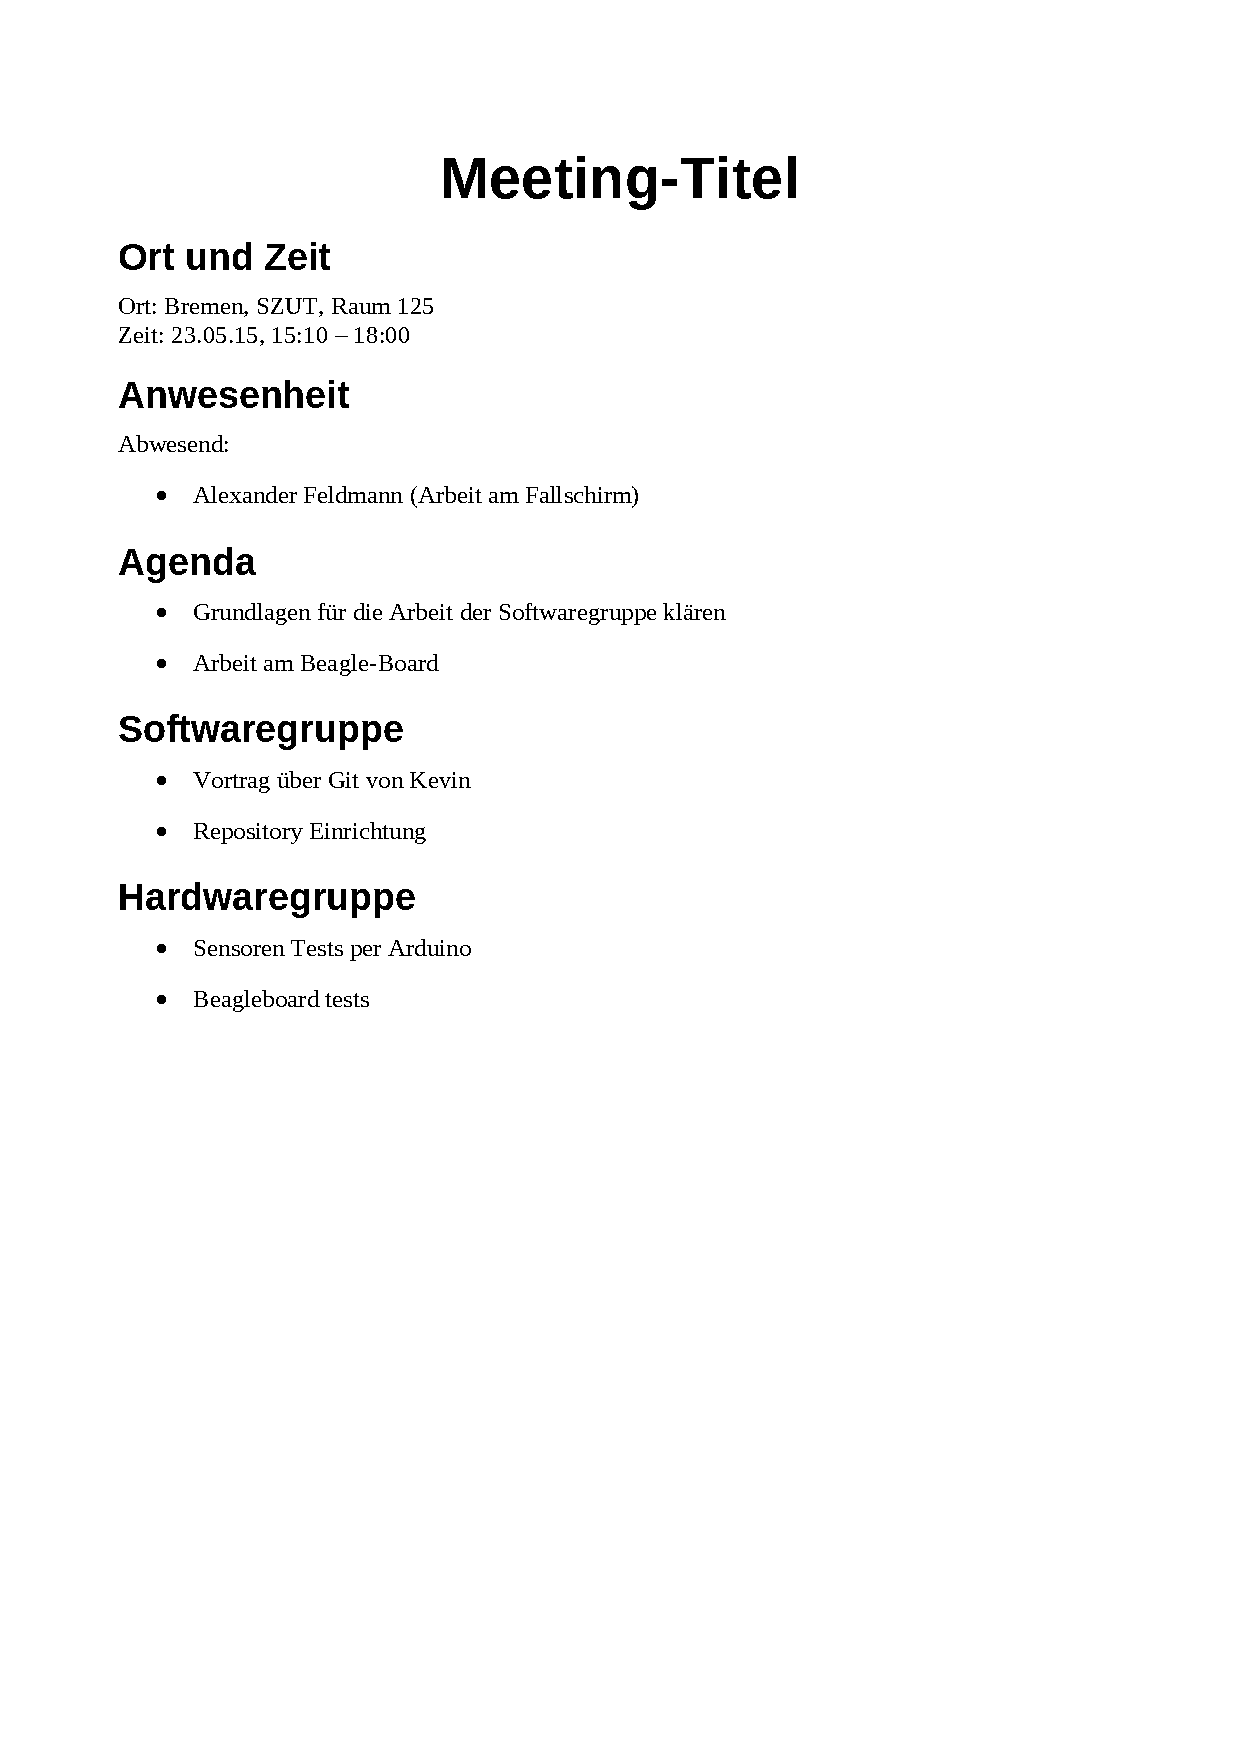
\includepdf{8_Anhang/Protokolle/150204_Meeting_Protokoll}%
\newpage
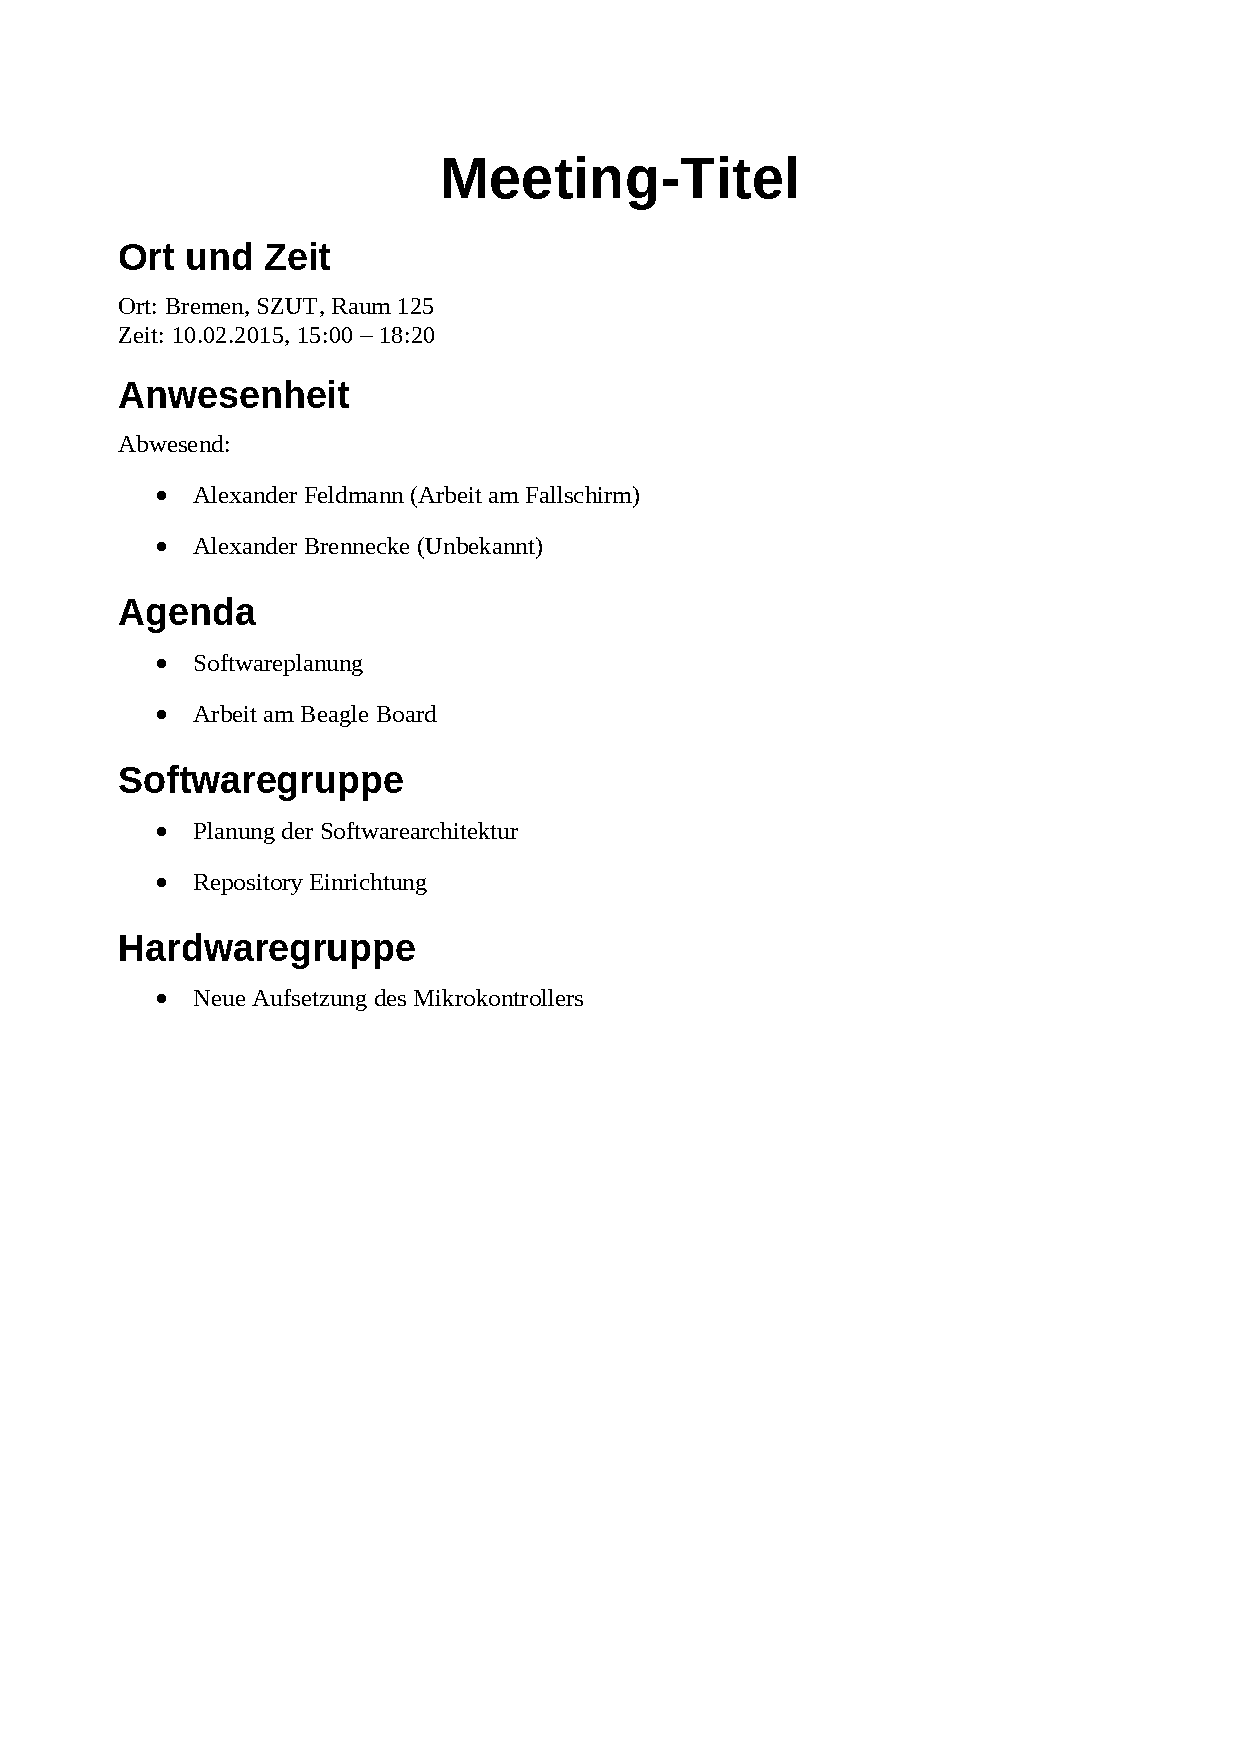
\includepdf{8_Anhang/Protokolle/150210_Meeting_Protokoll}%
\newpage
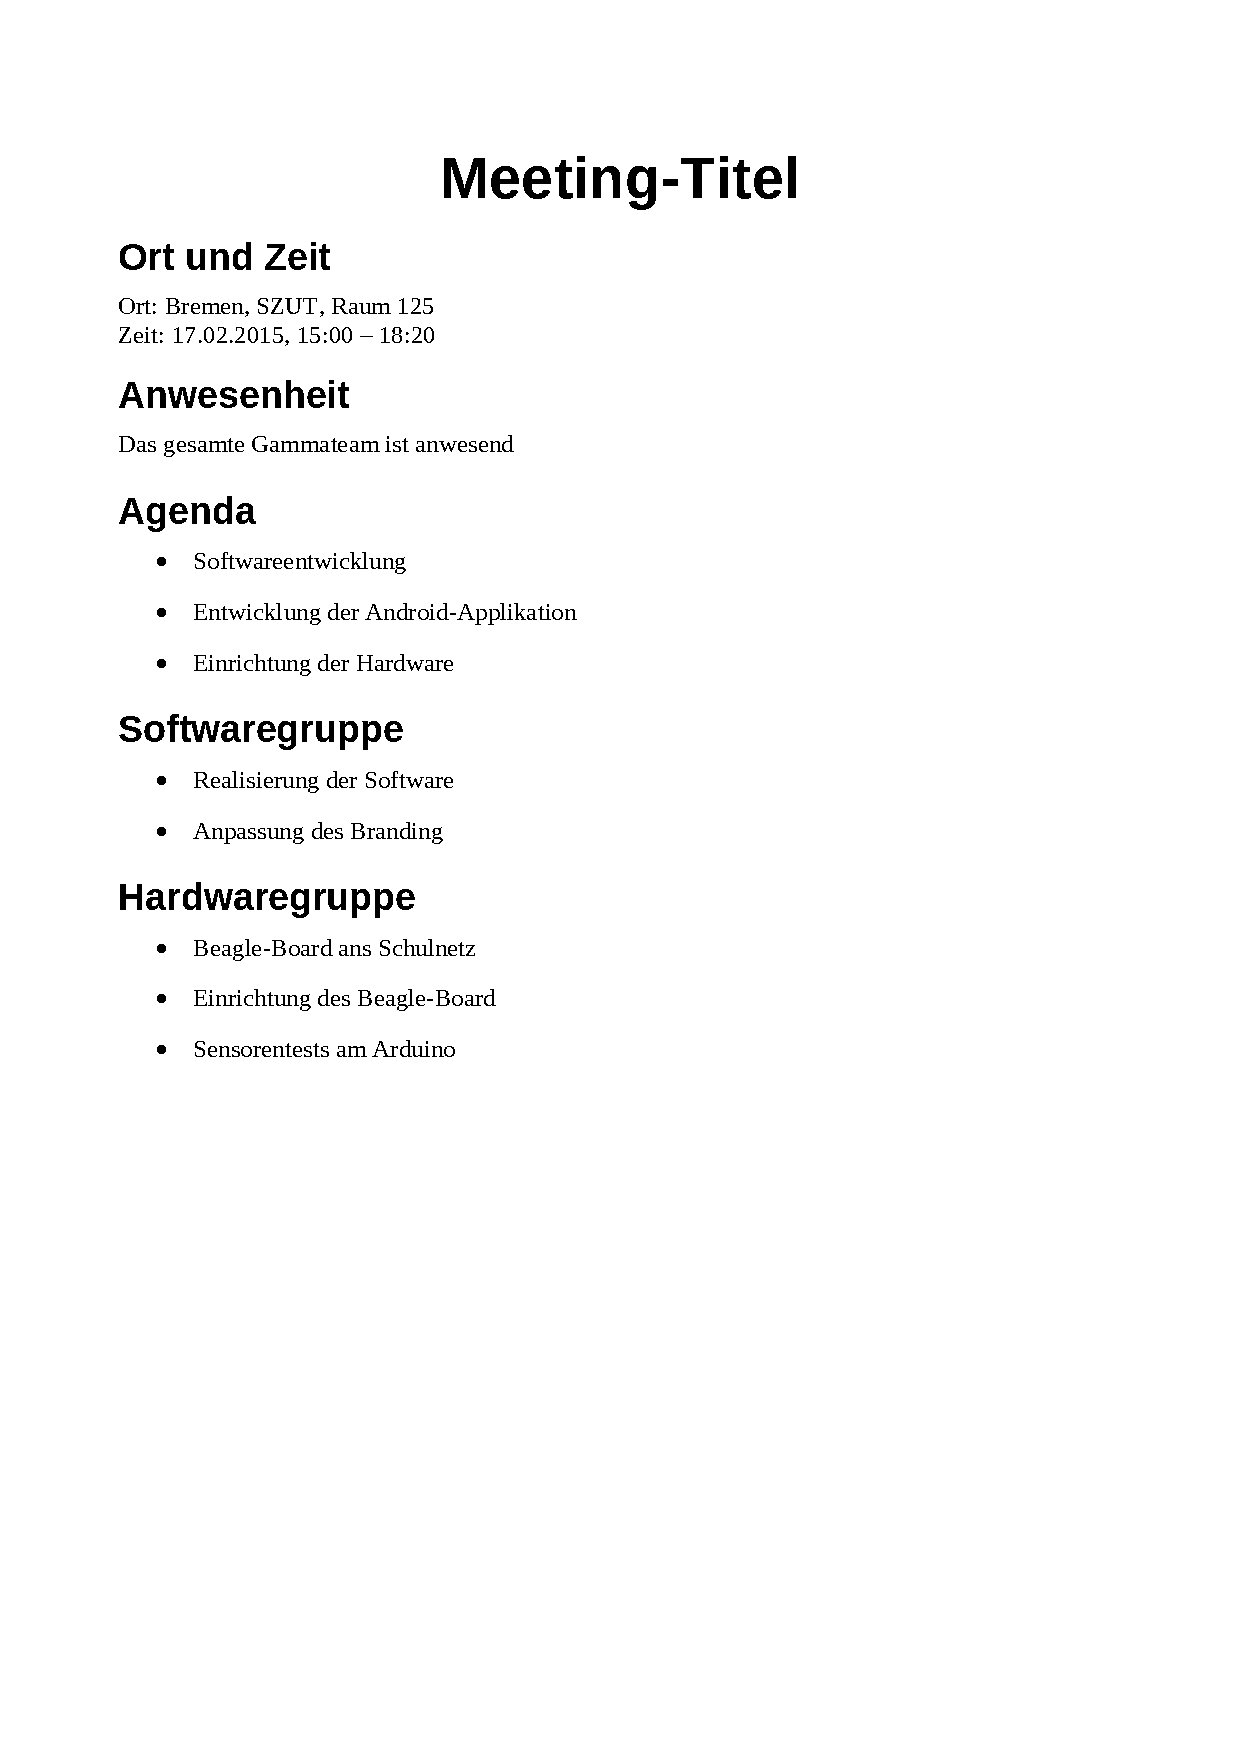
\includepdf{8_Anhang/Protokolle/150217_Meeting_Protokoll}%
\newpage
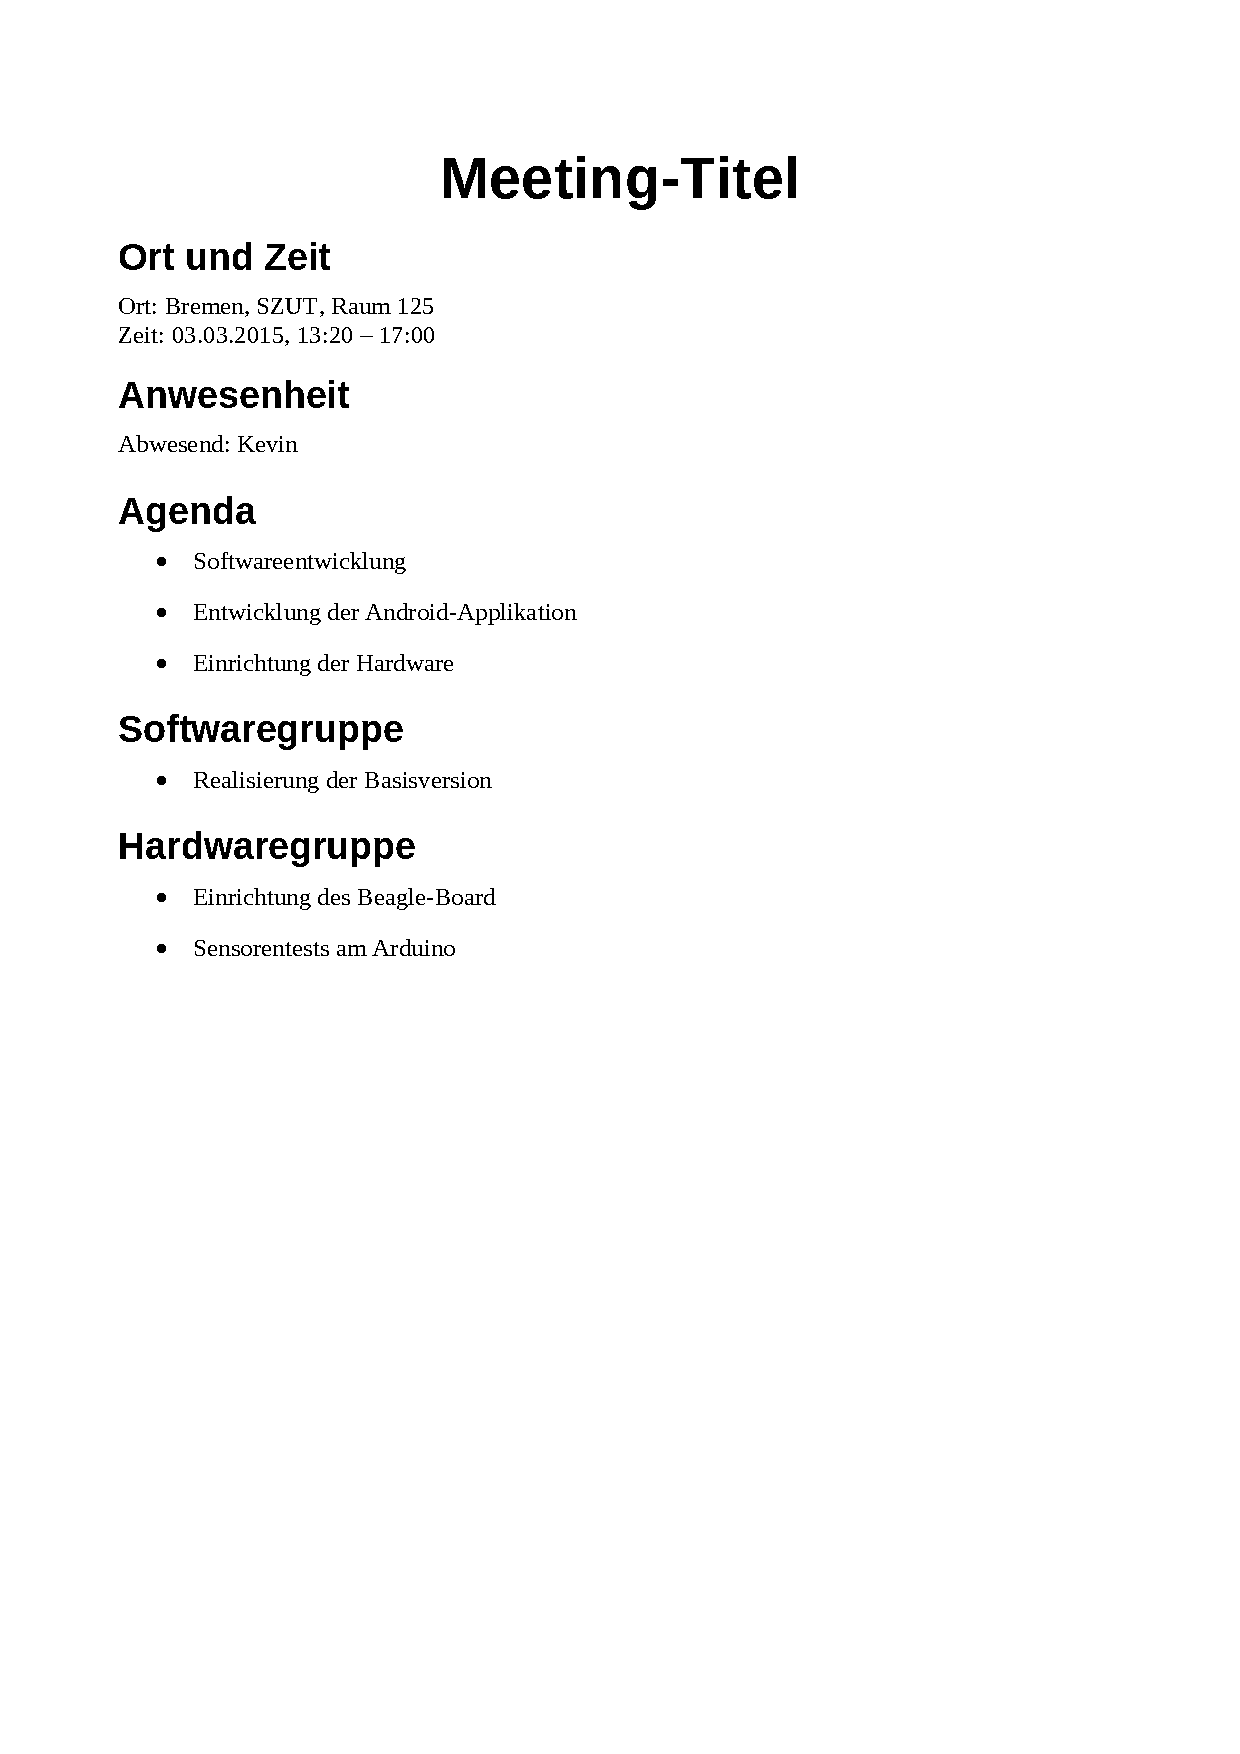
\includepdf{8_Anhang/Protokolle/150303_Meeting_Protokoll}%
\newpage
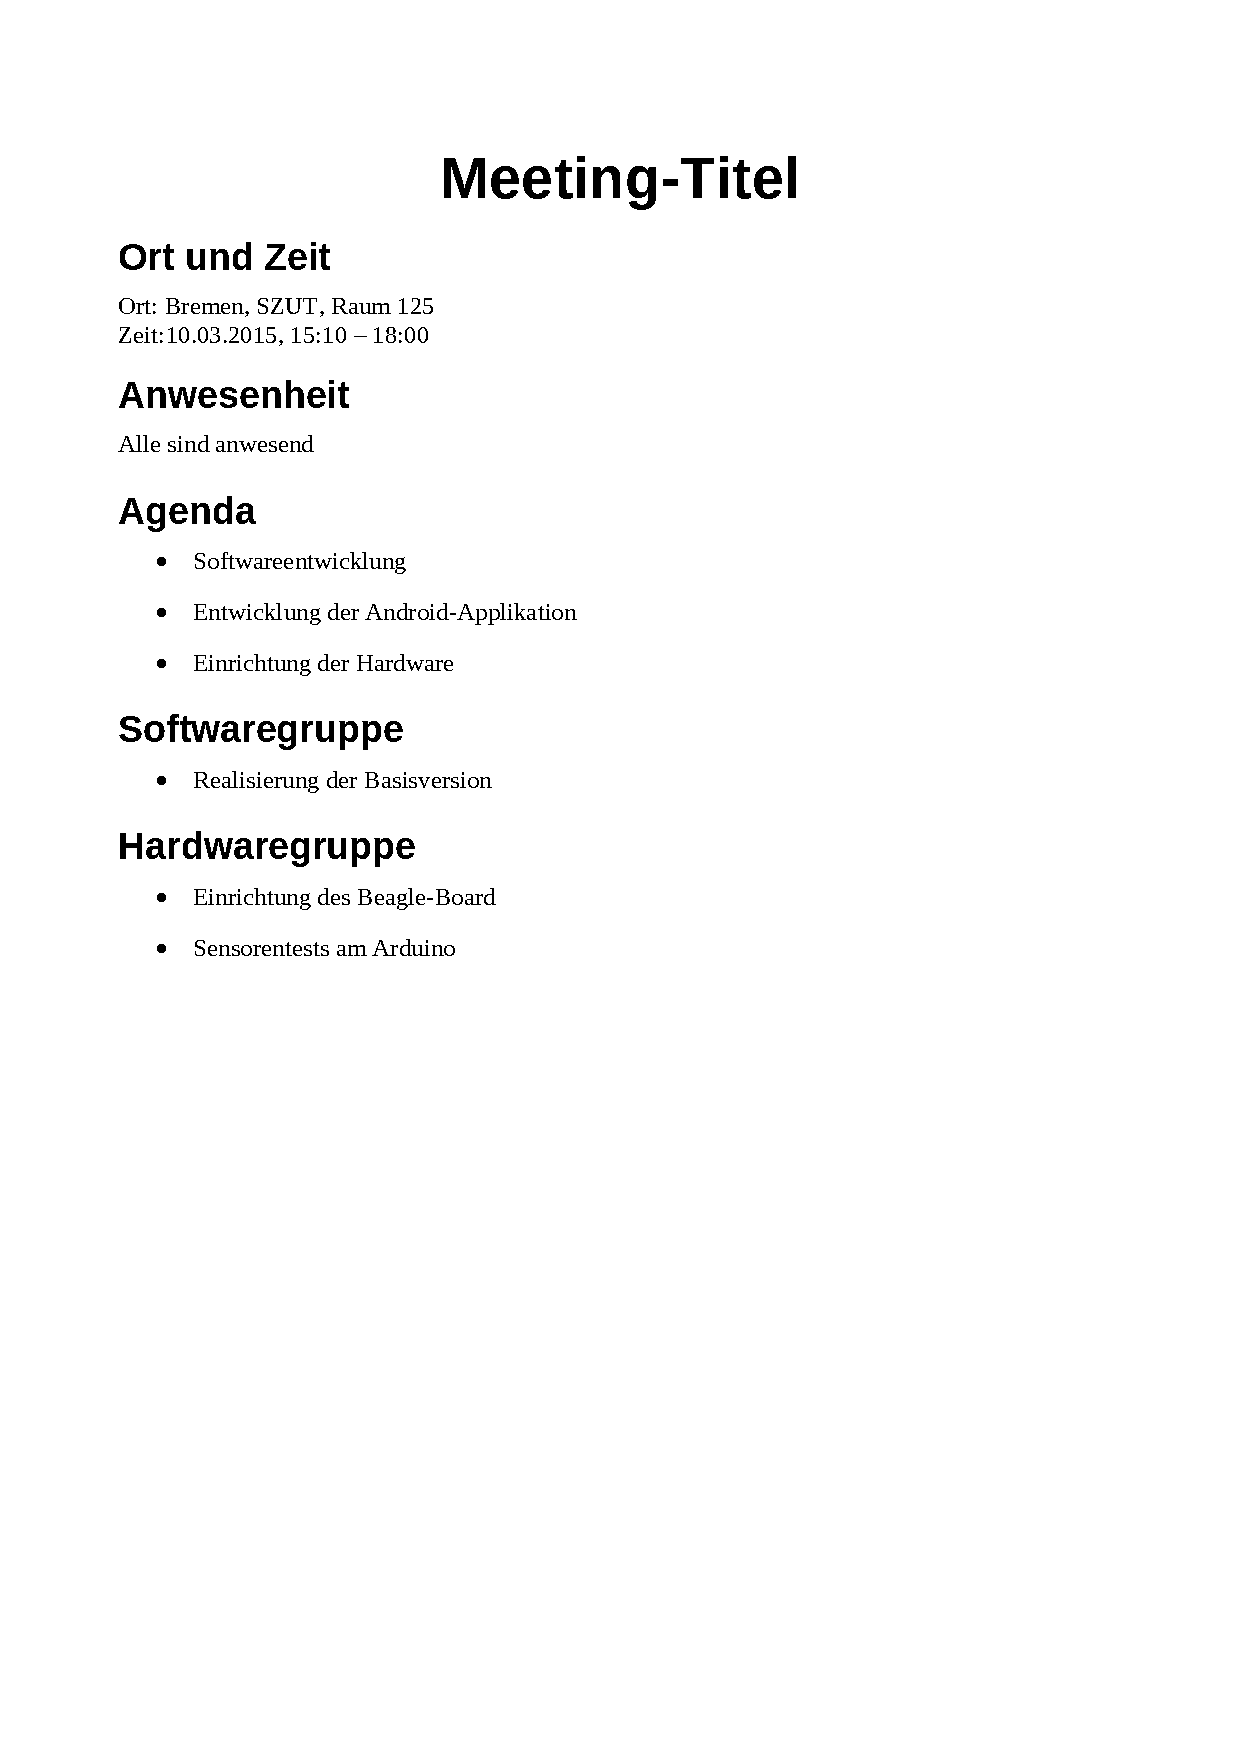
\includepdf{8_Anhang/Protokolle/150310_Meeting_Protokoll}%
\newpage
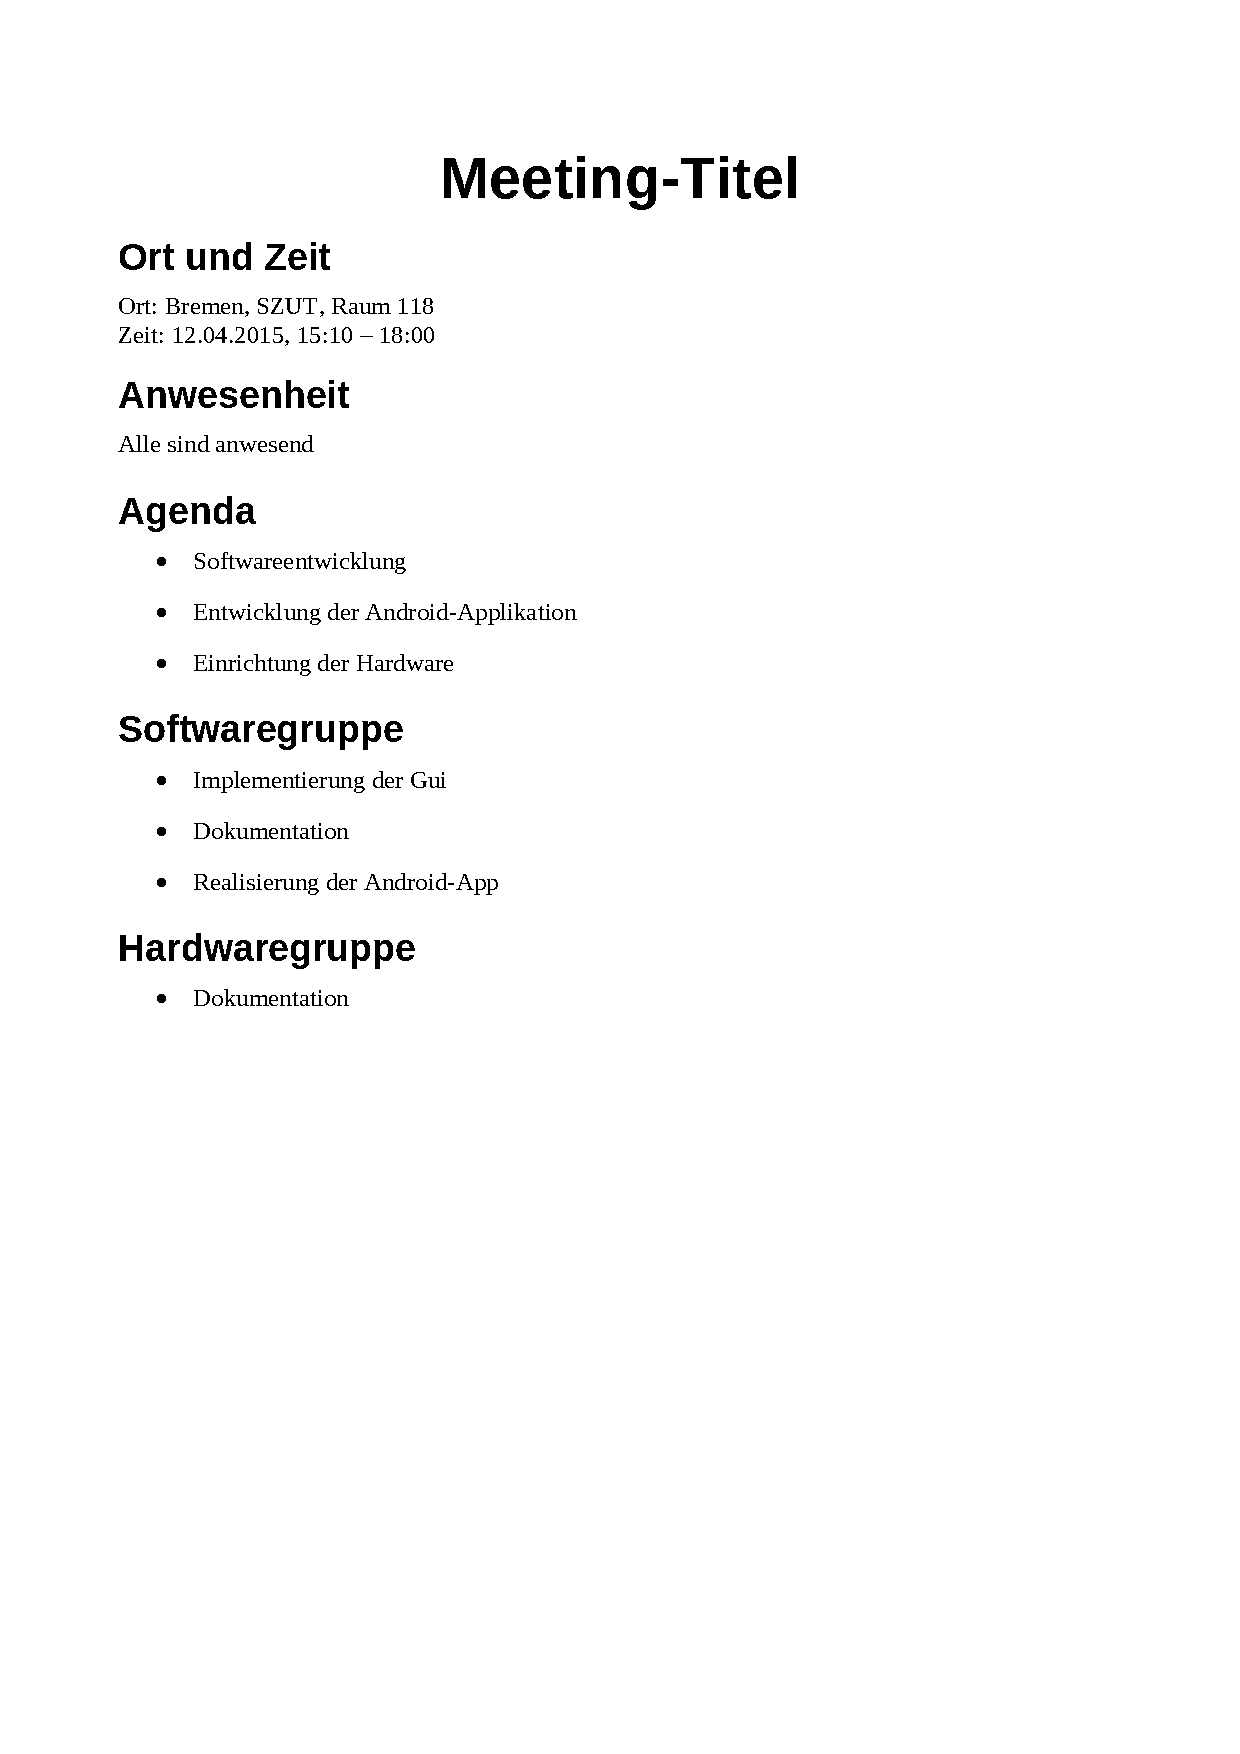
\includepdf{8_Anhang/Protokolle/150317_Meeting_Protokoll}%
\newpage
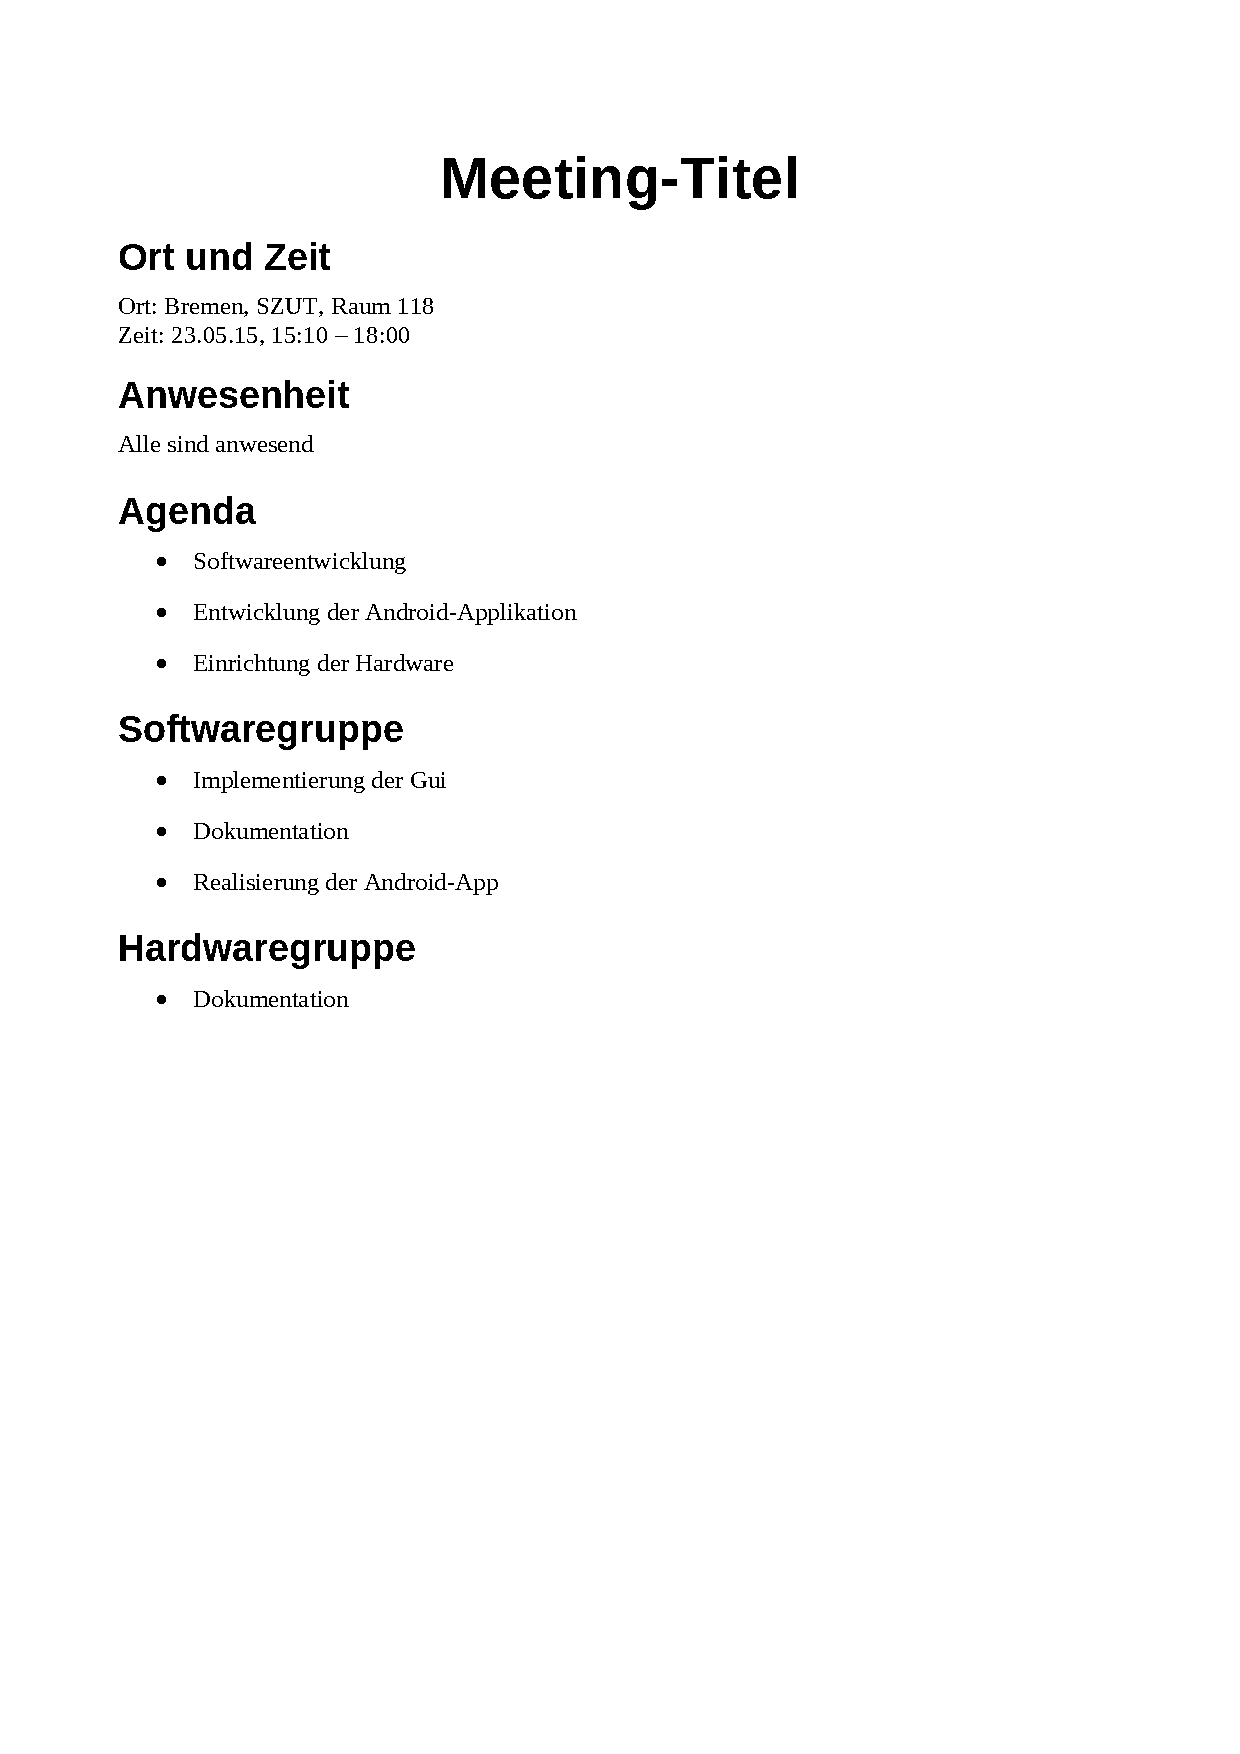
\includepdf{8_Anhang/Protokolle/150412_Meeting_Protokoll}%
\newpage
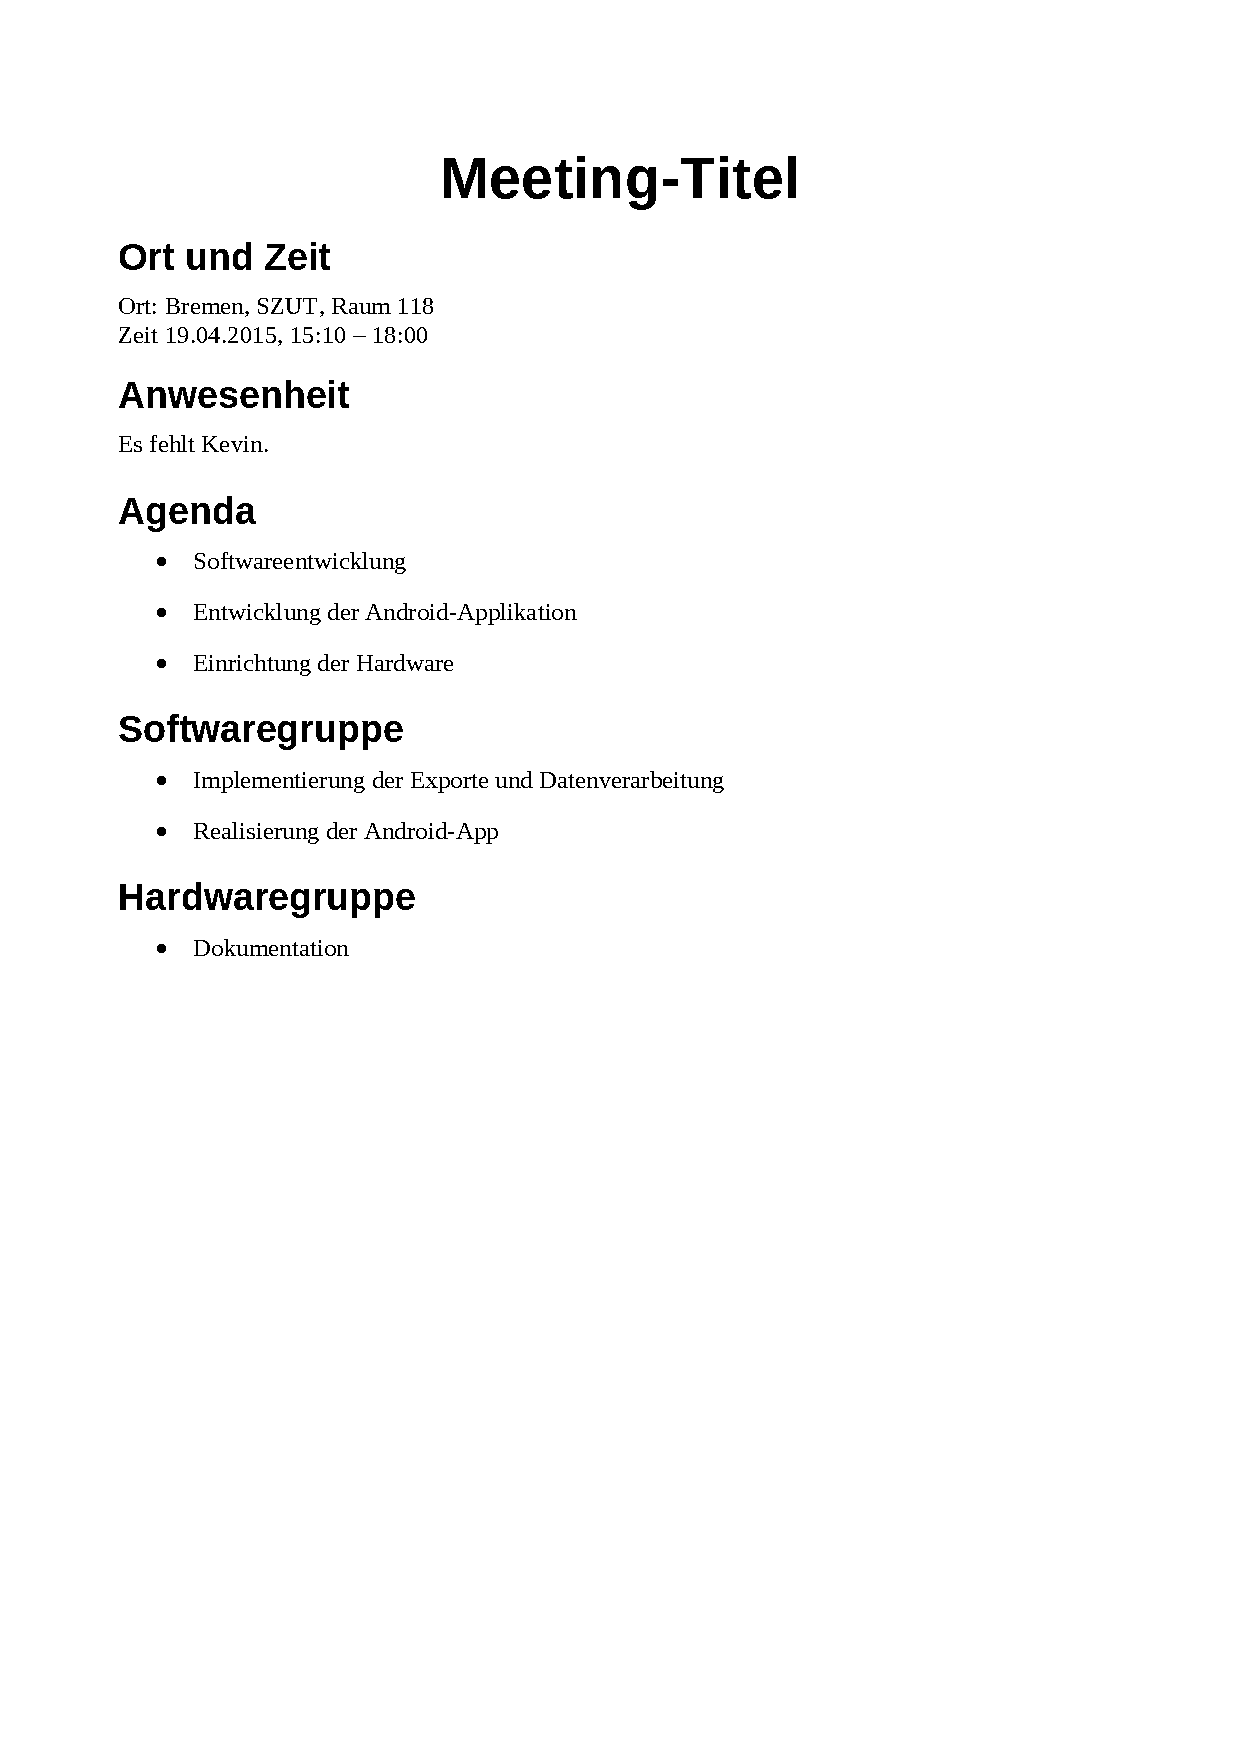
\includepdf{8_Anhang/Protokolle/150419_Meeting_Protokoll}%
\newpage
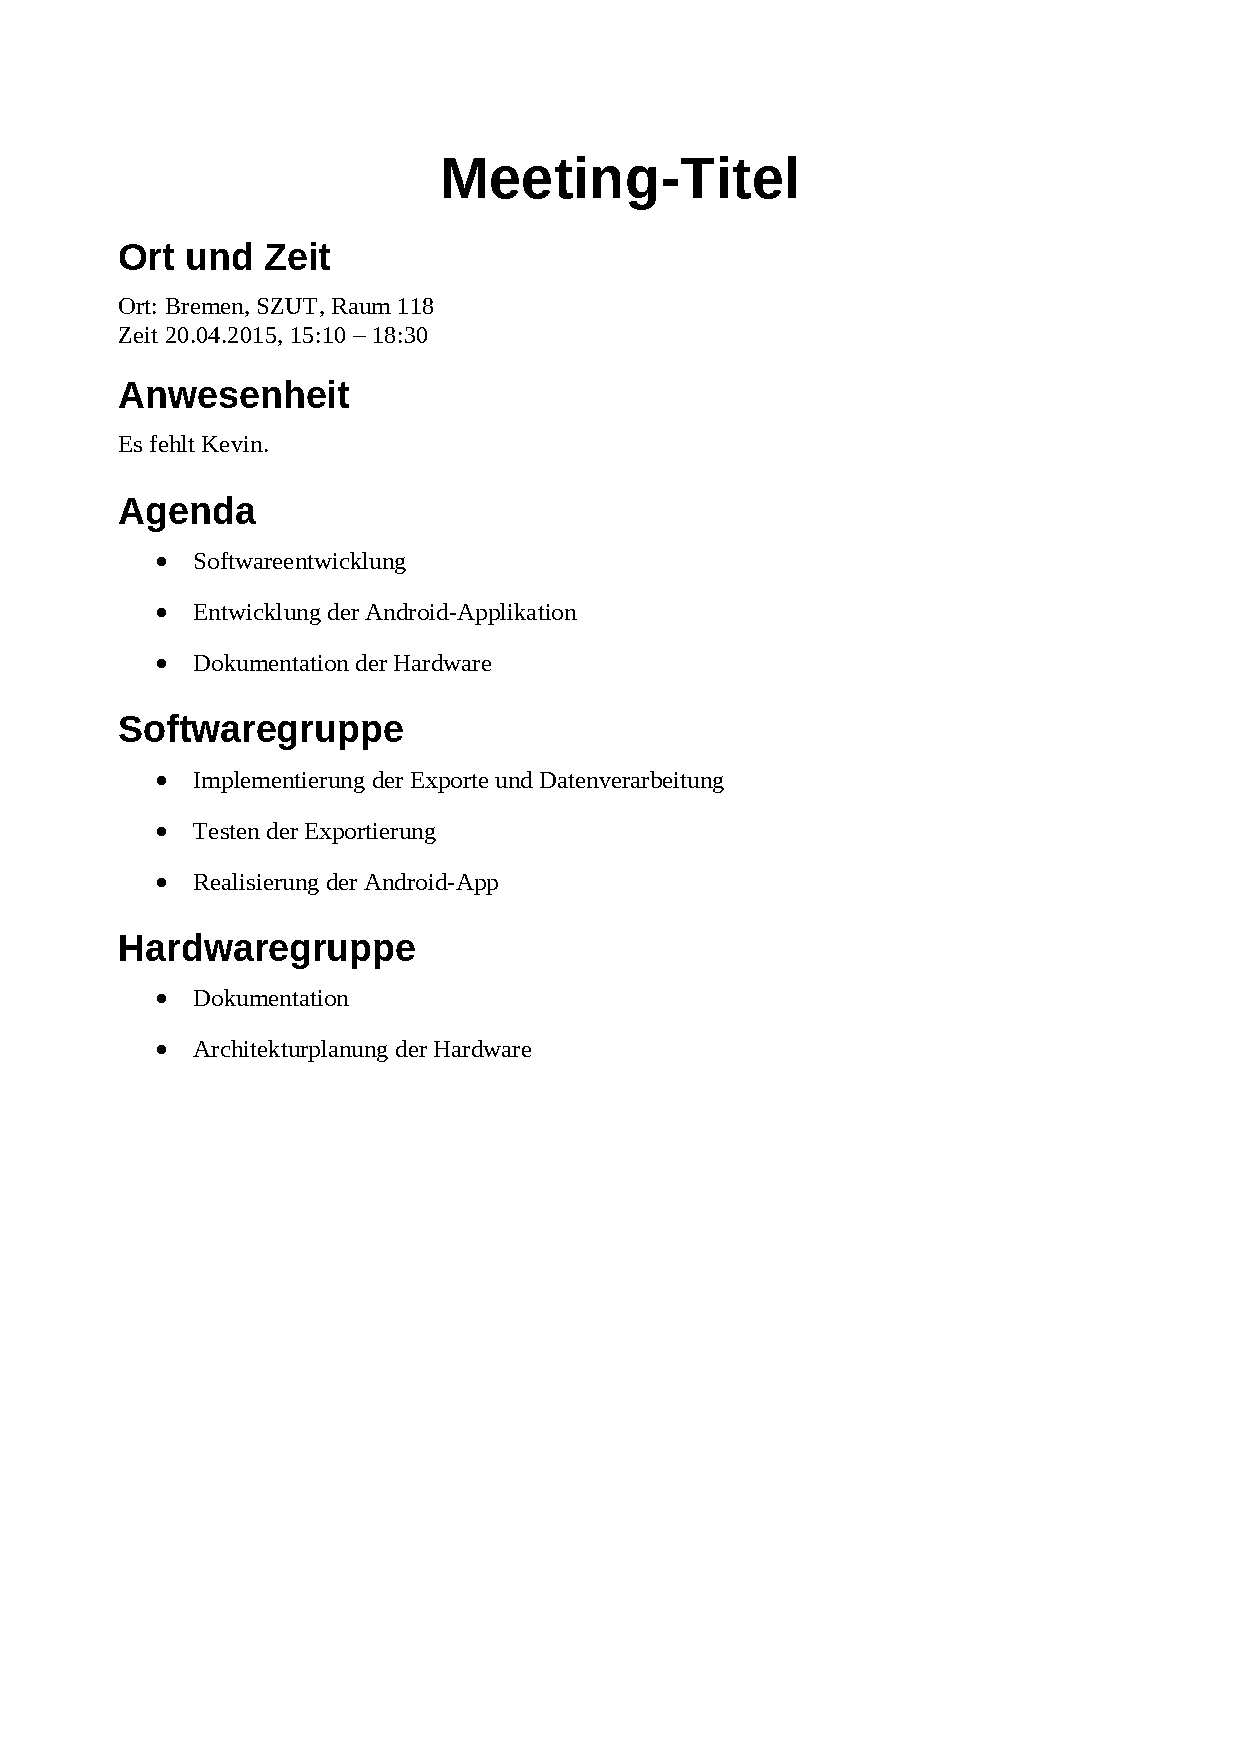
\includepdf{8_Anhang/Protokolle/150420_Meeting_Protokoll}%
\newpage
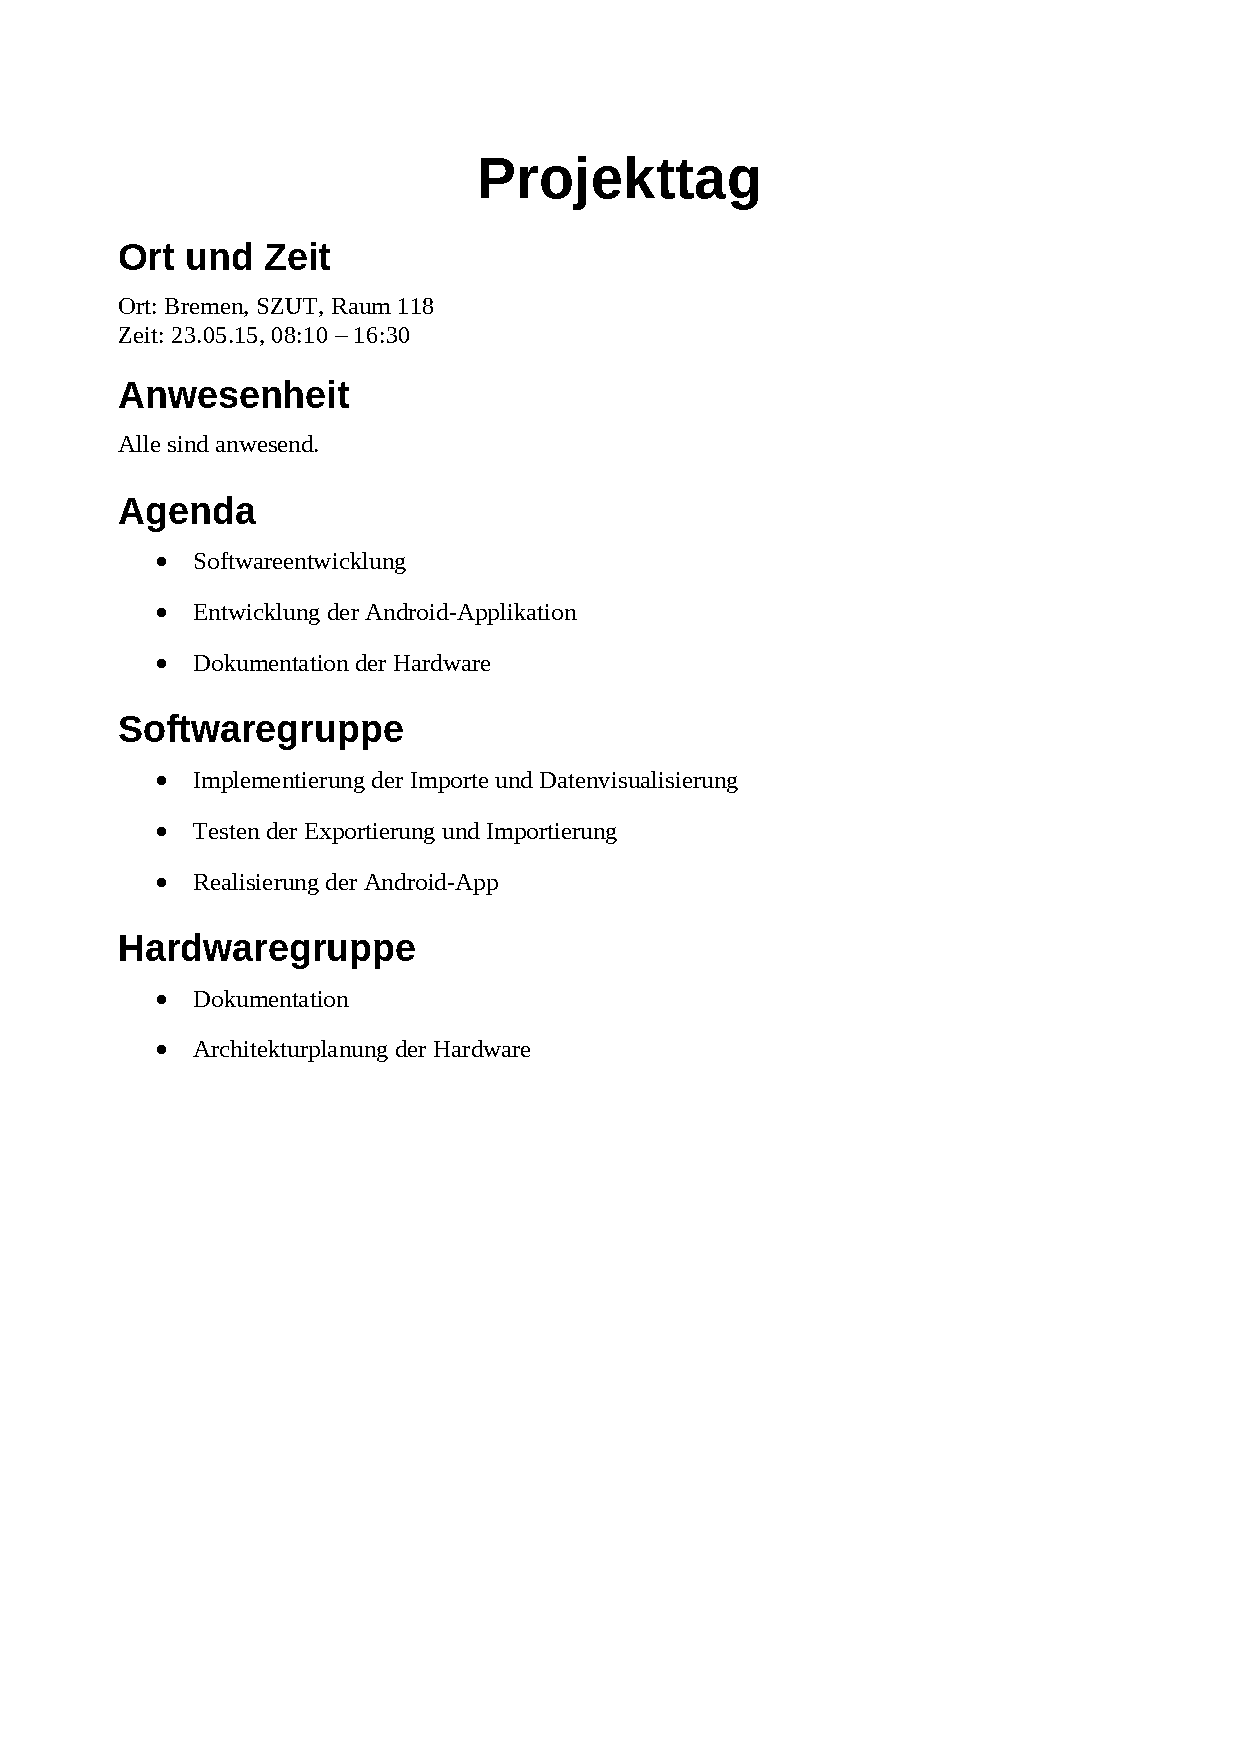
\includepdf{8_Anhang/Protokolle/150426_Meeting_Protokoll}%
\newpage
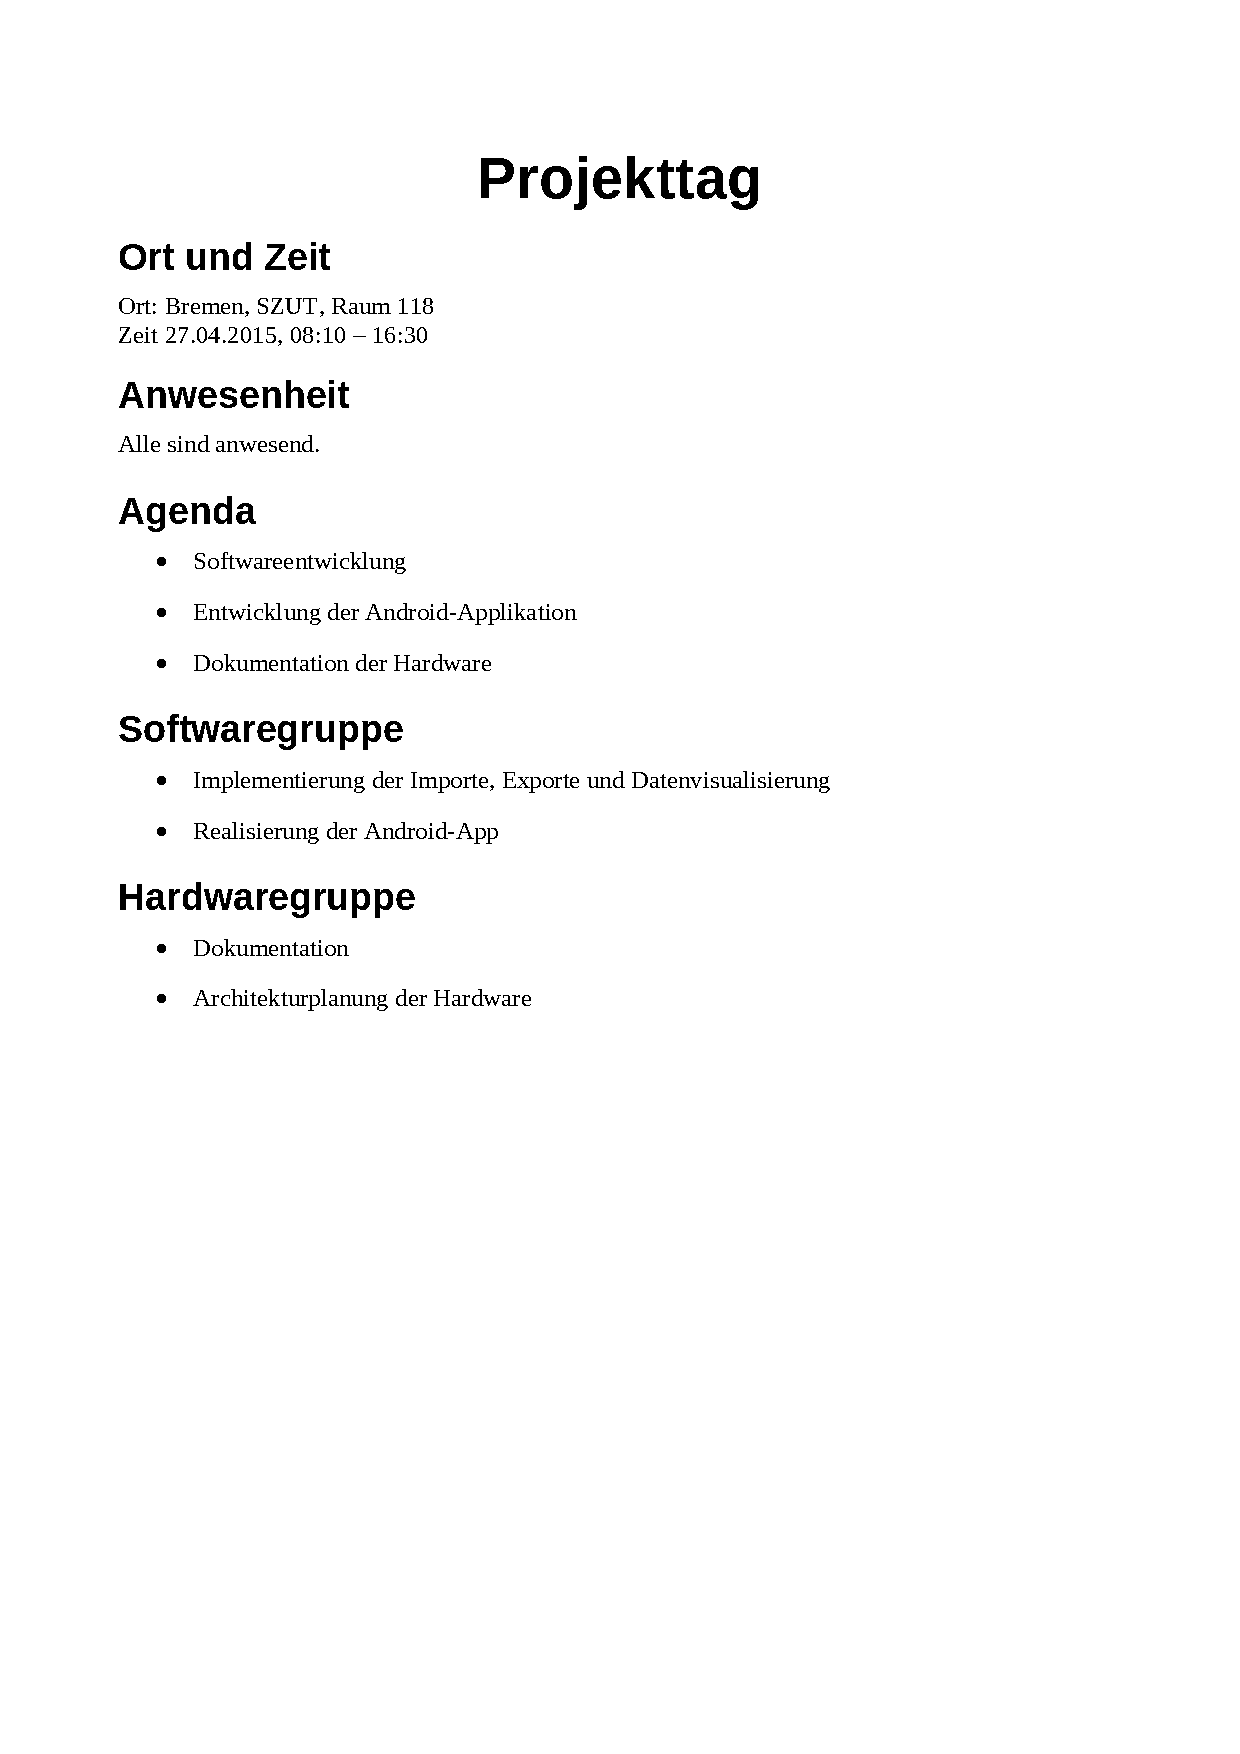
\includepdf{8_Anhang/Protokolle/150427_Meeting_Protokoll}%
\newpage
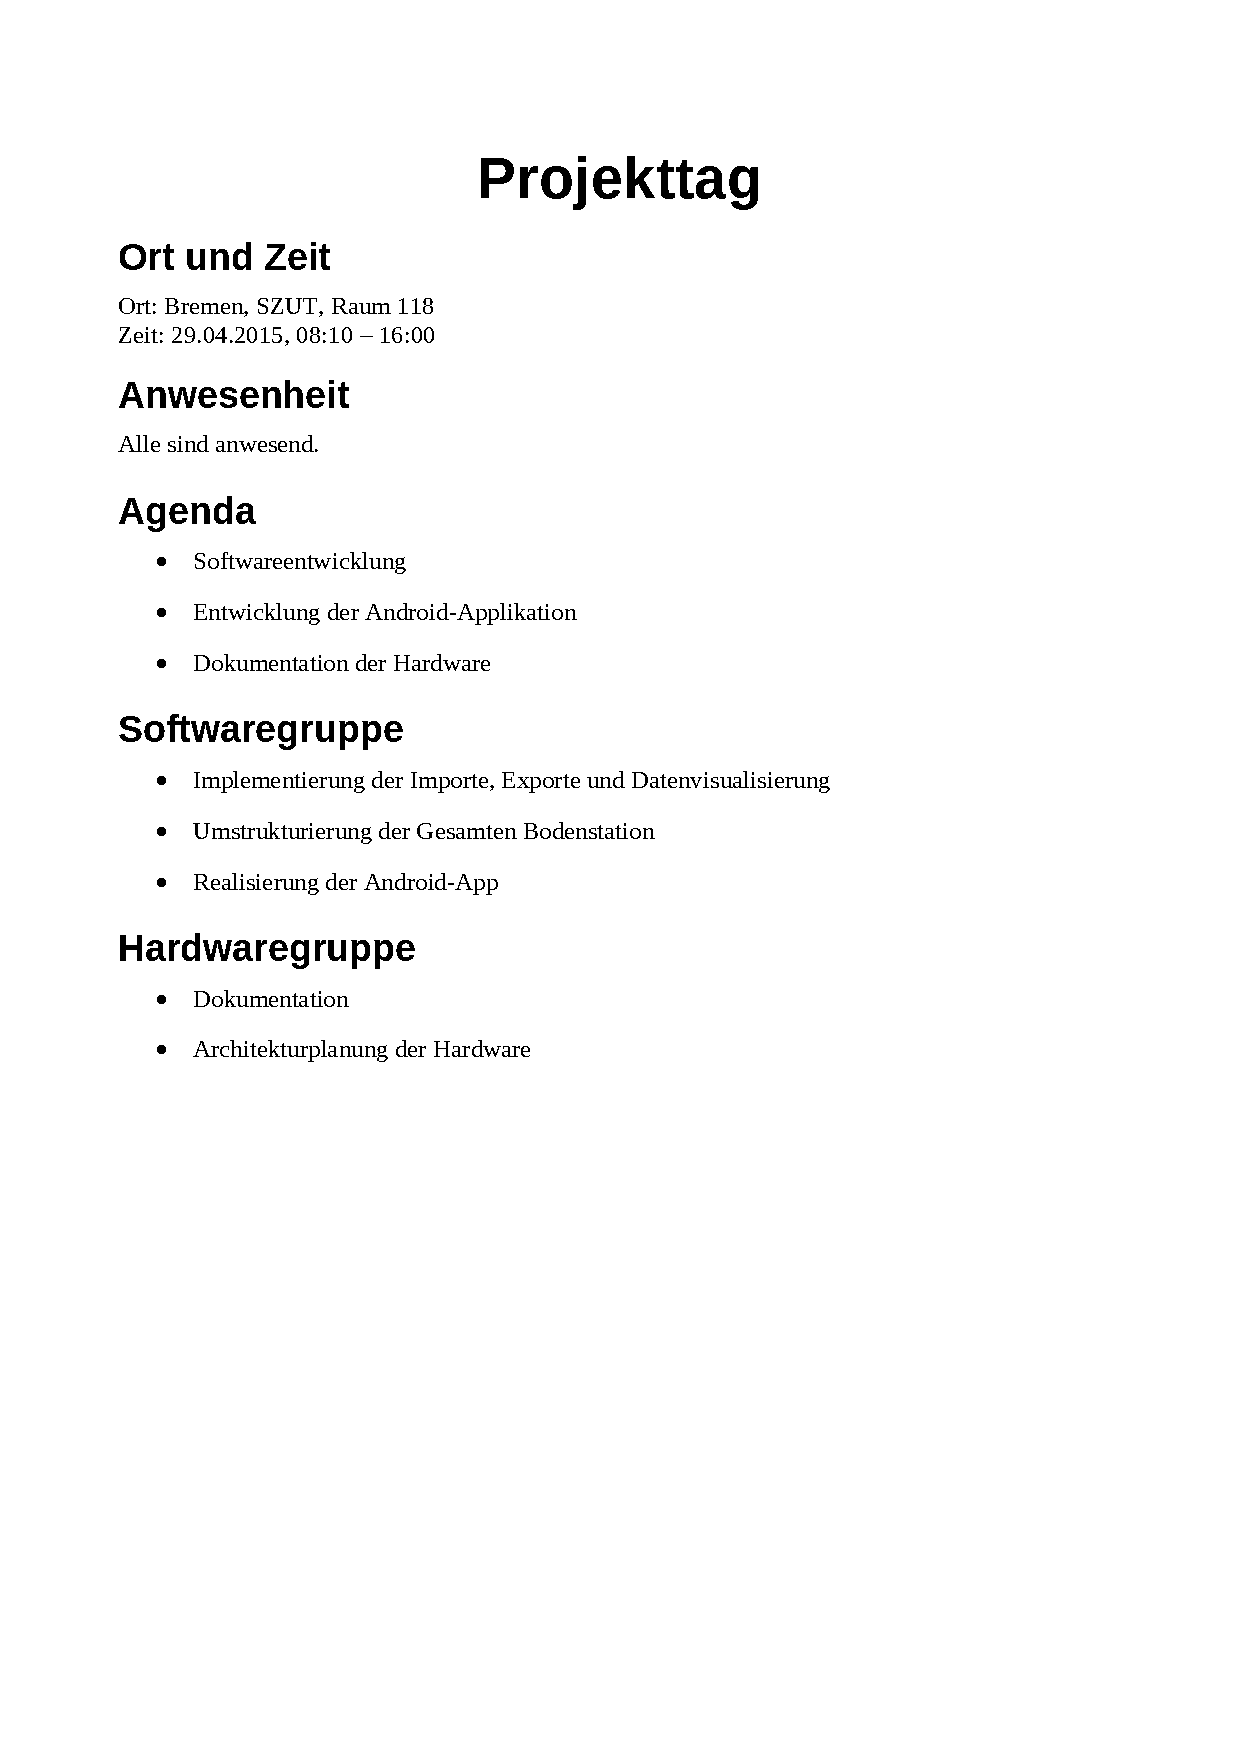
\includepdf{8_Anhang/Protokolle/150429_Meeting_Protokoll}%
\newpage
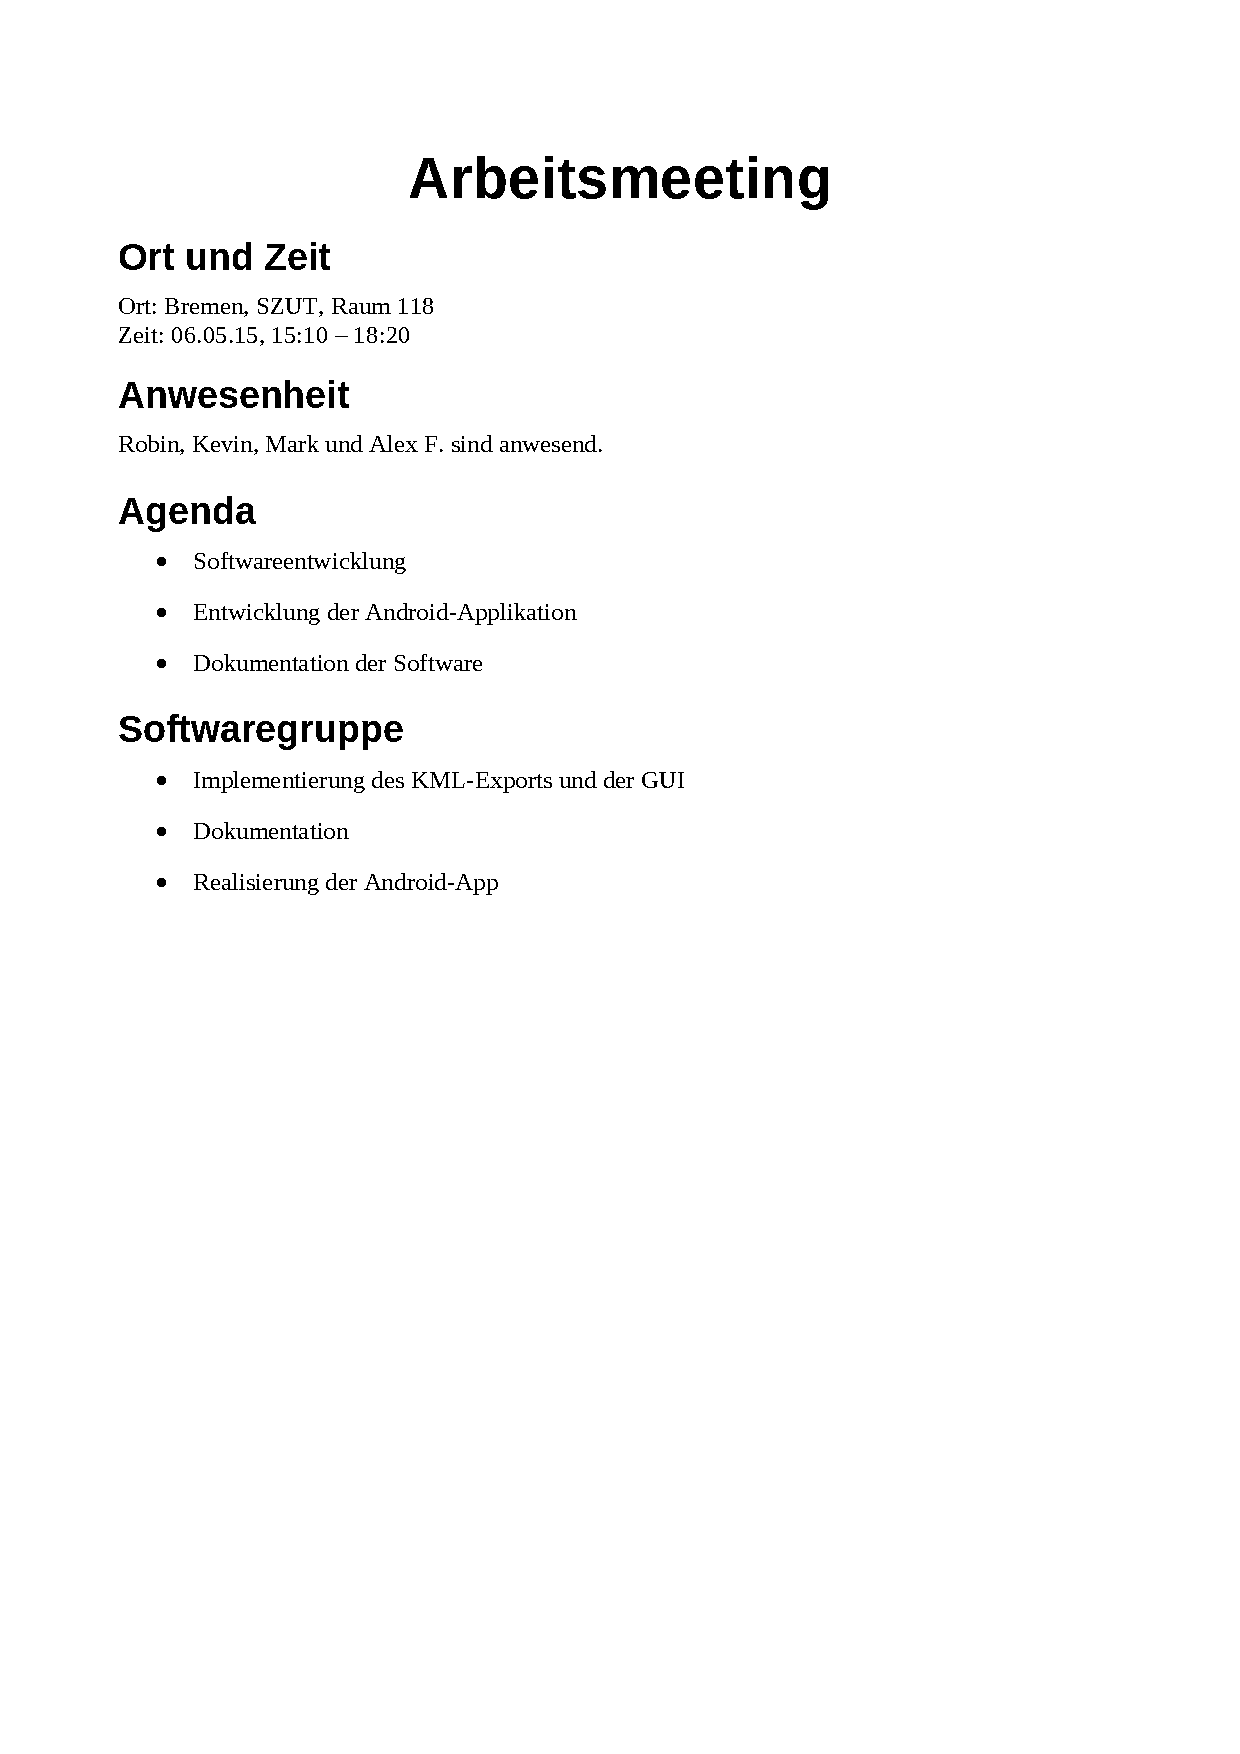
\includepdf{8_Anhang/Protokolle/150506_Meeting_Protokoll}%
\newpage
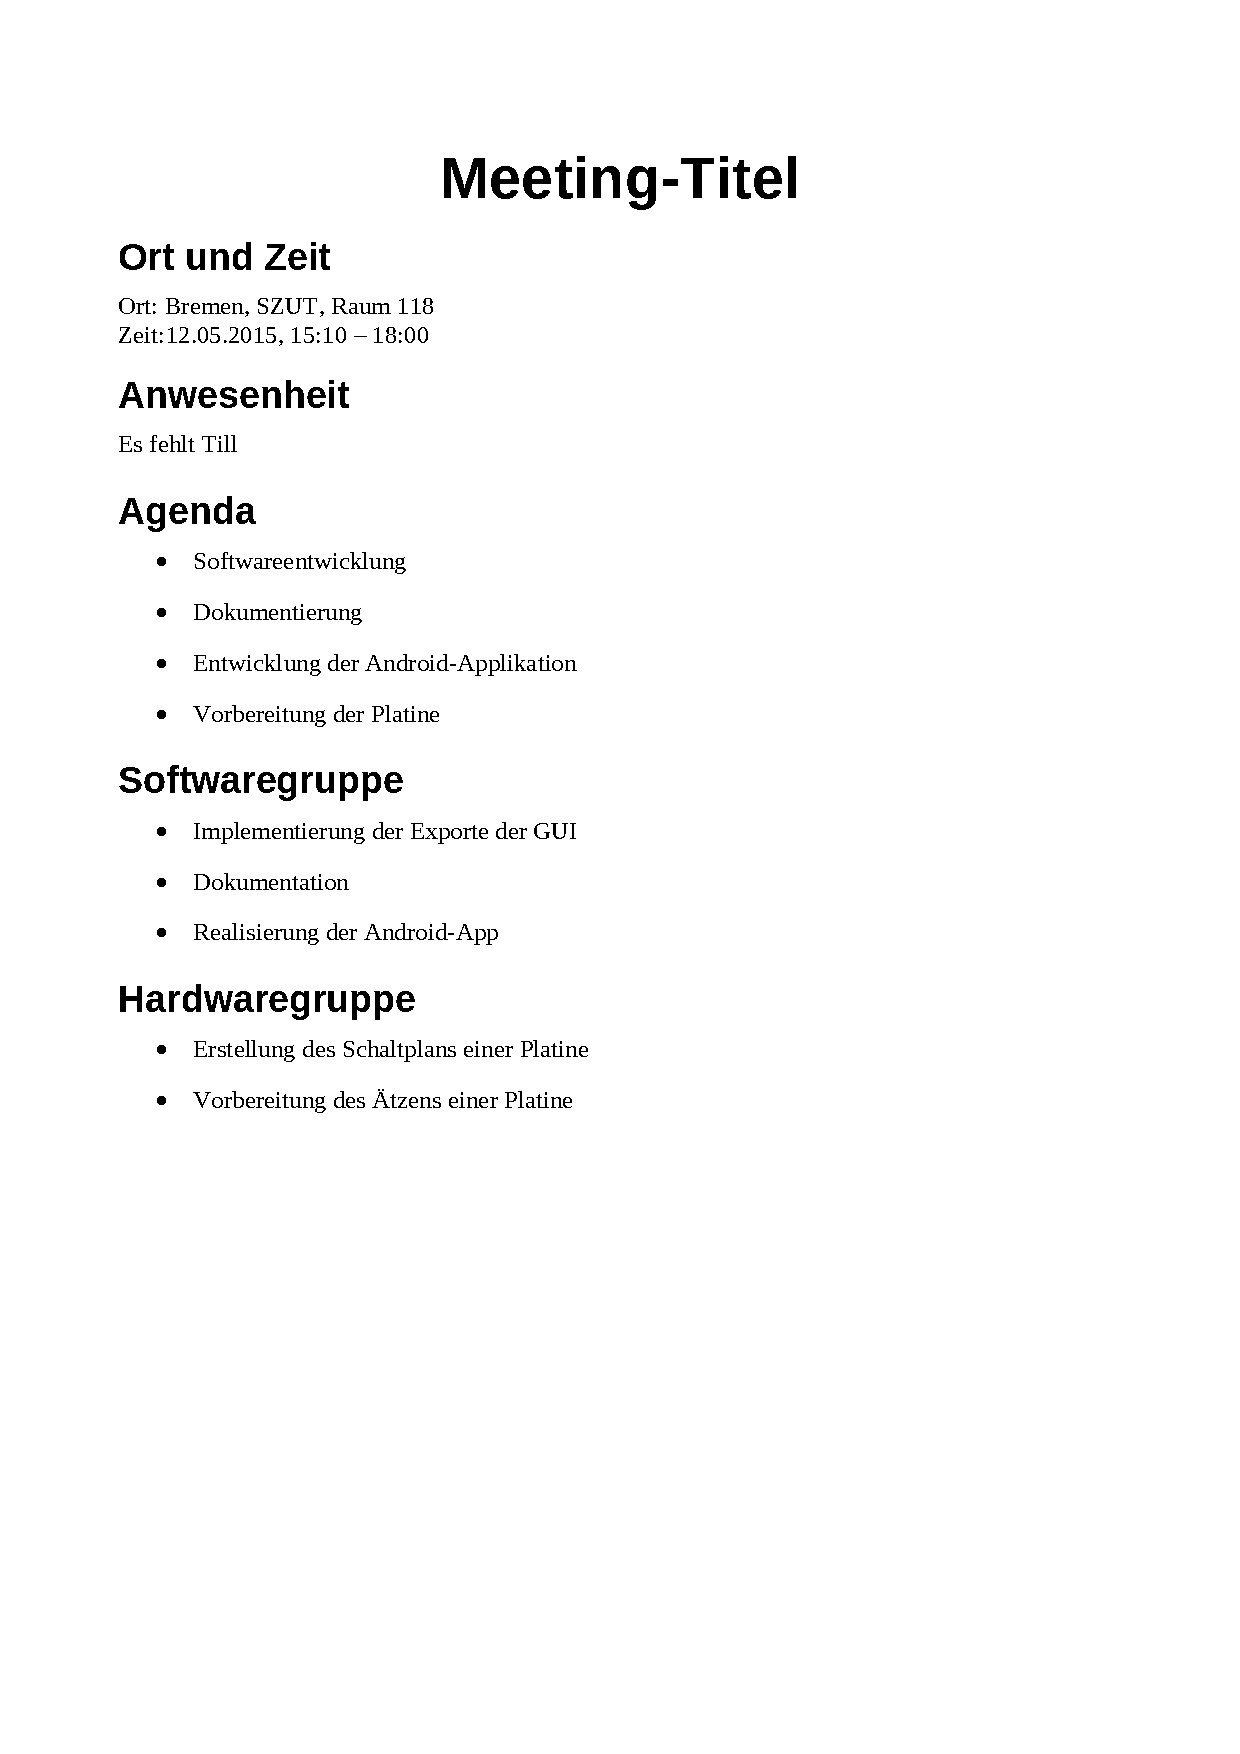
\includepdf{8_Anhang/Protokolle/150512_Meeting_Protokoll}%
\newpage
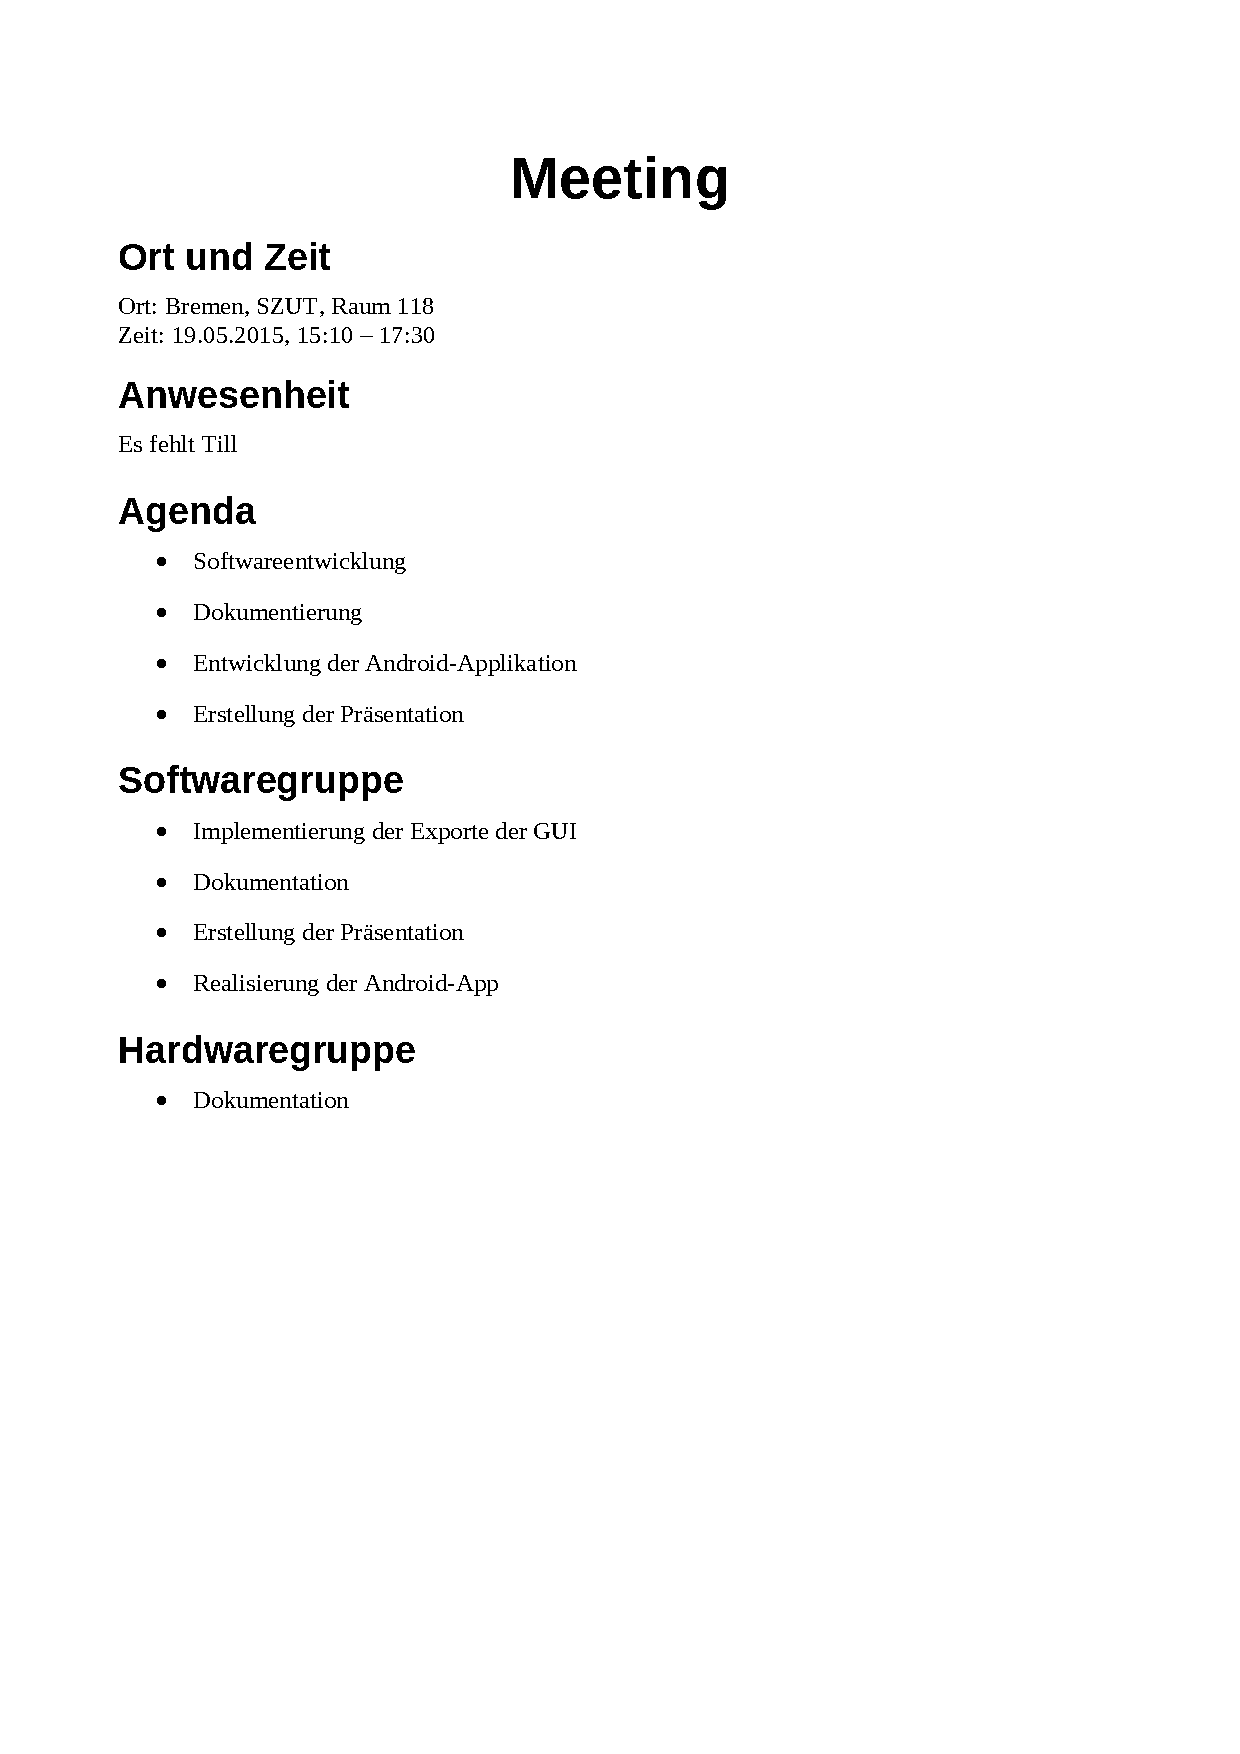
\includepdf{8_Anhang/Protokolle/150520_Meeting_Protokoll}%

\begin{comment}
0

{140921,141022,141202,141203,150106,150204,150210,150217,150303,150310,150317,150412,150419,150420,150426,150429,150506,150512,150520,150522} {

\foreach \i in {00, ..., 999999}%
    \edef\FileName{\i\_Meeting\_Protokoll}%     The % here are necessary to eliminate any
    \FileName%
    \IfFileExists{\FileName}{%  spurious spaces that may get inserted
    \includepdf[width=0.8\textwidth]{8_Anhang/Protokolle/\FileName}%
}%
}%

\end{comment}

